%
% This magic lets the Makefile create both the one-column version
% and the two-column version without the need to edit this file
%

\documentclass[11pt,letter]{article}
\usepackage{simson}

\newcommand{\be}{\textit{bulk\_extractor}\xspace}
\newcommand{\citeN}[1]{\cite{#1}}

\begin{document}
\title{A Survey of Digital Forensic File Recovery and File Type Identification Techniques}
\author{Simson L.\ Garfinkel}
\maketitle
\pagenumbering{arabic}

Over the past decade \emph{digital forensics} (DF) has grown from a trade
practiced by technicians working for law enforcement
organizations and into scientific discipline. Today DF  researchers are
making slow but steady progress on scientifically challenging
problems; DF research is presented at conferences
and published in peer-reviewed journals; and there is a growing
collection of both tools and reference data sets designed to promote
DF education and help validate new research techniques. Because of
both the scale and the diversity of their domain, DF researchers and
practitioners are necessarily at the forefront of some of the most
challenging problems in computer science today, including ``big data''
analysis, natural language processing, visualizations, and
cybersecurity. 

Broadly construed, DF applies the process and goals of \emph{forensic
  science} to the study of all things digital---and specifically to
digitized information that might be found on computers, cell phones,
storage devices and  computer networks during the course of a
criminal investigation. Compared with traditional ``blood and
bullets'' forensics, DF poses significant challenges for three primary
reasons: information on a computer system can be changed without 
trace; the scale of data that must be analyzed; and the variety of
data types that an investigator can encounter. Just as a traditional forensic investigator must be
prepared to analyze any kind of smear or fragment, no matter the
source, a DF investigator must be able to make sense of any data that
might be found on any digital device anywhere on the planet. In
practice, this is a very difficult proposition.

Much of what we now call DF got its start in the 1980s
as computer systems were increasingly involved in criminal acts.
From its inception, DF served two different
purposes. First, in many cases computers contained evidence of a
crime. In these cases the crime took place in the physical world
and the computer was all but incidental---except for the fact that
computerization made the evidence harder for
investigators to analyze than paper records. 

The second class of cases are those in
which the crime was inherently one involving computer systems, such as
computer hacking. In these cases, investigators are hampered
by the technical sophistication of the systems and the massive amount
of evidence to analyze.

DF is powerful because computer systems are windows into the
past. Many digital systems retain vast quantities of
information---either intentionally, in the form of log files and
archives, or inadvertently, as a result of software that does not
cleanly erase memory and files after it runs. As a result, it
is frequently possible for investigators to recover old email
messages, chat logs,   Google search terms and other kinds of data
that were created
weeks, months, or even years in the past. Such contemporaneous records
can reveal an individual's state-of-mind or intent \emph{at the time
  the crime was being committed}.

But whereas pre-computer evidence such as handwritten letters and
photographs could be photographically reproduced and given to attorneys, judges and juries, computerized evidence
requires special handling and analysis. In part this is because
electronic data are easily changed, damaged or erased if
handled improperly---for example, simply turning on a consumer GPS
may cause the device to erase critical evidence. Additionally,  computers
frequently harbor hidden evidence that may only be evident when
specialized tools are used---for example, a digital camera may appear to have
30 photos, but examination by an expert may reveal that another 300
deleted photos can be recovered.

As the preceding paragraphs make clear, today the field of digital
forensics is largely \emph{tool-based} and
\emph{investigator-centric}. 
That is, the requirements of DF are driven 
by what investigators need to perform digital
investigations\citep{walls-levine-effective-digital-forensics}. Convictions
are frequently the
measure of success. In many cases there is a considerable gap between
what is theoretically possible and what is necessary. That is, even
though there may be an intellectual desire to analyze and explain every last byte
on a piece of subject media\cite{garfinkel:every-last-byte}, there is
rarely a reason to do so.

\section{Digital Forensics}

% http://www.tex.ac.uk/cgi-bin/texfaq2html?label=complist
\subsection{Collection and Preservation} 
Before data can be analyzed, they
  are taken from the field (the ``scene of the crime''),
  stabilized and preserved to create a lasting record. 

When recorded on a hard drive or camera card, these bytes are groups in
  blocks called \emph{sectors} that are typically 512 or 4096 bytes in
  length. A sector is the smallest block of data that a drive can read
  or write. An email message might require 10 or 20 sectors to
  store; a movie might require hundreds of thousands. Depending on the
  arrangement of other files on the device, the sectors can be stored
  as a single sequential stream or they can be fragmented into many
  different locations. Other sectors contain information that the
  computer uses to find the stored information: such bookkeeping
  information is called ``file system metadata.''

  Each sector on the disk has a unique identifying number, called
  the sector's \emph{logical block address} (LBA). An Android phone
  advertised as having ``8GB'' of storage has eight billion bytes or roughly 15
  million sectors.  To preserve the data on a computer or phone, each of these sectors
  must be individually copied out of the phone or off the hard drive and
  stored on another computer in a single file called a \emph{disk image}
  or \emph{physical image}. This file, which contains every single byte
  stored on the target device, naturally includes every
  visible file on the media. But the physical image also records
  invisible files as well as portions of files that have been deleted
  but not yet overwritten by the operating system. 

  For typical desktop or laptop computers, collection and preservation
  is performed with a program called a \emph{disk imager}, of which there
  are many. Disk imager  are tested by the Computer Forensic
  Tool Testing Program (CFTTP) at the National Institute of Standards and
  Technology (NIST) Information Technology Lab (ITL) to make sure that
  they accurately copy all of the data off the subject
  device. Although it might seem straightforward, the task is
  complicated by the possible presence of bad sectors and ``hidden''
  storage, the need for the program to detect and accurately report
  the drive being unplugged, and other issues that may seem
  inconsequential but which can be very significant when a disk image
  is being used as the basis of a criminal prosecution. 

\textbf{TK: Add about testing and error rate}

  In the case of network forensics, it is the actual data
  sent over the network connection that are preserved. This means that network forensics
  equivalent to a wiretap---and in fact network forensics equipment is
  increasingly used for wiretaps by law enforcement. 

%  Today's computer networks carry information in blocks
%  called \emph{packets} which are typically between 50 and 1500 bytes
%  in length. Network collection is performed with tools called
%  \emph{packet sniffers} or \emph{network forensic analysis tools}
%  (NFATs)\cite{613756}. These tools intercept the packets that are
%  sent down a wire (or through the air) and copy them into a file
%  called a ``packet trace'' or a ``PCAP'' (packet capture) file.  

  Increasingly the random access memory (RAM) associated with computer
  systems is also being subjected to forensic investigation. RAM is
  difficult to work with, as it changes very quickly and is lost when
  a computer is turned off. RAM must also be captured with a special
  program (a ``memory imager'') and is stored in its own special kind
  of file called a ``memory dump.'' Although memory can be extracted from all
  kinds of computer systems, including desktops, laptops, cell phones,
  as well as network communications equipment such as wireless
  routers, each of these systems uses different kinds of internal
  structures, so software designed to analyze one may not analyze another.


\subsection{Examination and Extraction} Working with the preserved data, an
  examiner will explore for any information that might be
  relevant to the investigation at hand. 

  When performing disk forensics, files that can be seen from within
  the computer's own operating system are called ``allocated files''
  because the storage associated with the files is allocated to that
  purpose. On many system it is also possible to recover files that have
  been deleted but whose previously allocated sectors have not yet
  been overwritten or otherwise used for another purpose. These
  sectors are said to contain \emph{deleted files}, \emph{residual data}, or
  \emph{digital trace evidence}.

Most examinations are performed
  with tools that can extract user files from the disk image, search for files that contain a specific word or phrase
  in a variety of human languages, and even detect the presence of
  encrypted data. One common technique is to arrange all of the
  information chronologically and create a timeline that shows when
  each file on the disk was modified or last accessed.

 Another 
  technique is to review every directory and file and look for
  things that seem out-of-the-ordinary. 

Relevant data are then
  extracted from the preserved system so that they are easier to
  analyze---for example, an individual file may be sent to a linguist
  for translation. In the military this process of examination and extraction
  is frequently called \emph{exploitation}.

  There are many tools for performing examination. The Sleuth Kit\cite{sleuthkit} is
  an open source tool that can decode Windows, Macintosh, Linux, XBox,
  and Android
  file systems, recovering both allocated and deleted
  files;   Volatility\cite{volatility} can analyzing memory dumps from a
  variety of different systems.

\subsection{Analysis} Once potentially relevant information is
  extracted, an analyst will construct one or more hypotheses that
  uses the digital evidence to explain possible past activities. A
  hypothesis may draw from multiple digital devices---an email message
  sent from a desktop computer to a cell phone, for example---or the
  hypothesis may incorporate events in the physical world, like a
  power failure or theft. During this phase a good analyst will also
  try to construct alternative hypotheses that are consistent with the
  evidence but which point to different conclusions. In Europe it is
  popular for examiners to perform an Bayesian analysis and estimate
  the probability of each hypothesis based on the available data.

  Many examination tools can perform some kind of analysis, but there
  are also commercial tools that specialize at this task. Examples
  include Analyst Notebook\cite{analysts_notebook} and
  Palantir\cite{palantir}, as well as general purpose tools such as
  Microsoft Excel.

\subsection{Reporting and Testimony} Finally, the analyst will
  produce a written report or give testimony in a courtroom. Remember,
  judges and juries can't examine digital evidence for
  themselves---even if they had the training and the technical skills
  to do so, performing their own analysis would be inappropriate:
  their role in the legal process is to evaluate the law, the evidence
  and make a legal determination, not to perform technical
  analysis. Reports and testimony must be
  \emph{complete}---they must describe the tools and procedures
  that were followed, clearly document what was found, and then
  separately provide the technical interpretation of the
  evidence. (For this very reason, Rule 704 of the US Federal Rules of
  Evidence, allow a DF expert to
  express an opinion on ``an ultimate issue to be decided by the trier
  of fact'' in most circumstances.)

\section{The Science of Technical Exploitation}

In the early 1990s there were no DF tools as we know them
today. Instead practitioners had to repurpose tools that had been
developed for other purposes. For example, backup software was
used for collection and preservation, while data recovery tools were used
for examining subject media. Although these approaches worked, they lacked control,
repeatability, and a known error rates---that is, examiners had no way
of knowing the accuracy of their results. 

In 1993 the US Supreme Court held in the case of Daubert v. Merrell
Pharmaceutical 
that any scientific testimony presented in court must be based on a theory
that is testable; that has been scrutinized and found favorable by the
scientific community; that has a known or potential error rate; and
that is generally accepted\cite{daubert}. This case didn't directly
kick off the demand for DF tools, but it did give DF practitioners
grounds for arguing that validated tools were needed not just as a matter
of good science and procedure, but as a matter of law. 

Since then there has been a steady development of techniques and the
incorporation of those techniques in a variety of tools. This section
presents several techniques for what has come to be called
\emph{technical exploitation}. The first two techniques---hashing and
file extraction---now dominate all DF processing. The next three
techniques---reconstruction of compressed data, memory parsing, and
fraud detection in multimedia---represent the next generation of DF
research that is leveraging new algorithms and signal processing
approaches to help address challenges facing DF practitioners today.

\subsection{Hashing}

Probably the single most transformative technical innovation in
DF has been the introduction of hash functions, first as a means for assuring the integrity of forensic data,
and later as a way to recognize specific files.

In computer science a \emph{hash function} is any function that maps a
sequence of zero or more characters (called a \emph{string}) to an
binary number of a specific fixed size---that is, a fixed number of
bits. A 16-bit hash
function can produce $2^{16}$ different hash values, while a
32-bit hash function can produce $2^{32}$ possible hash
values. Hash functions are designed so that changing a single
character in the input results in a completely different number. While
the pigeonhole principle guarantees that many different strings will
have the same hash value---called a \emph{hash
  collision}---the more bits in the hash has, the smaller the chance
of a collision.

Hashing was invented by H.\ P.\ Luhn in a 1953 IBM technical memo for
automated text processing. (Interesting fact: The name \emph{hash}
comes from the way hash functions are typically implemented as a
two-step process that first chops and then mixes the data, much in the
way that one might make hash in the kitchen.)

In 1979 Merkle proposed that hashes could be constructed as one-way
functions and used as the basis of digital signatures for certifying
documents\citep{merkle:79}.

One of the first and continuing uses of hashing in DF was to establish
\emph{chain-of-custody} for forensic data. Instead of hashing a
document or a file, the hash function is applied to the entire disk
image---that is, \emph{all} of the bytes extracted from a hard
drive. Many law enforcement organizations will create two disk images
of a drive and then computer the hash of each image.  If the values
match, then the copies are assumed to each be a true copy of the data
that were on the drive. The hash value is then included in the
official report. With the hash recorded, the image file can be copied
to a server at the police department, to an investigator's
workstation, or even given to a forensic expert working for the other
side. Any investigator with the data can calculate the hash and see if
it matches the original reported value. If the hashes match, the
investigator can be sure that not a single bit in the disk image has
been changed since the original image was recorded. Hashing is so
important that many DF tools can automatically validate an evidence
file by recomputing the hash and comparing it with a stored value.

A second use for hashing is to identify specific
files. This approach takes advantage of the property that it is
extraordinarily unlikely for two files to have the same
hash value. File hashes can thus be used to identify files in much the
same way that a person can be identified by their fingerprints. 

Today forensic practitioners distribute databases containing the file
hashes as a standard part of forensic processing. The best known of these data
sets is the National Software Reference Library Reference Data Set,
distributed by the National Institute of Standards and
Technology\cite{nist-nsrl-rds-march2012}. These data sets can be used
to identify \emph{known goods}, such as programs distributed as part
of operating systems, or \emph{known bads} such as computer viruses,
stolen documents and child of pornography. Recent work is now
applying cryptographic hashing to blocks of data smaller than
files\cite{garfinkel:sector-id}, taking advantage of the fact that
even relatively short 512-byte and 4096-byte segments taken from
files can be highly identifying. 

File and sector identification with hashing means that a hard drive
containing millions of files can be automatically searched against a
database containing the hashes of hundreds of millions of file hashes
in a relatively short amount of time---perhaps just a few hours. Importantly, the search can be done without any human
intervention.

\subsection{Files Recovery and File carving}

Many forensic investigations start with the examiner looking for
files belonging to the computer's previous user. But what is a file?

On modern digital systems, a \emph{file} is a sequence of
\emph{bytes}. Files therefore
have \emph{contents} and a \emph{length}, but they do not necessarily have other
information that computer users typically associate with files, such
as a \emph{file name} or a \emph{modification date}. These attributes
are called \emph{metadata} (literally ``data about data'')
and are stored by the computer's \emph{file system}, but are not
strictly part of the file. (Some operating systems even allow a single
file to have multiple names or timestamps, further complicating the
issue.)

\emph{Allocated files} are files that can be viewed
through the file system and whose contents will not under normal
circumstances be inadvertently overwritten by the operating
system. The word ``allocated'' refers to the \emph{disk sectors} in
which the file's content is stored. The sectors are allocated in the
sense that they are dedicated to the file and cannot be assigned to
other files and overwritten. Allocated files are present in either the
file system's \emph{root directory} or a \emph{sub directory}. These
are the files that a user typically sees with the Windows Explorer or
the Apple Finder. Many DF tools allow the examiner to see allocated
files present in a disk image without having to use the computer's
native operating system. This makes it possible to maintain forensic
integrity of the evidence.

One of the major technical DF innovations of the
past 15 years has been approaches for
recovering a file after it is deleted. These are not simply files that are in
a ``trash can'' or ``recycle bin''---these are the files after the
trash has been emptied. So-called \emph{deleted files} can be
recovered because many operating systems don't actually overwrite the
sectors of files when the user deletes them. Instead, the file names
are hidden and the storage associated with the files is
\emph{deallocated}. Similar techniques can also be used to
recover deleted email messages in Microsoft Outlook ``\texttt{.pst}'' files.

Sometimes a file's content remains on the computer's hard
drive, in memory, or on external media but the metadata that could be
used to recover the deleted file is overwritten or otherwise lost. Recovering
these kinds of data requires a technique called \emph{file carving}.

File carving appears to have been invented by independent security researcher
Dan Farmer and was incorporated into the first open source digital
forensics tool called The Coroner's Toolkit written and released by Farmer and IBM
researcher Wietse Venema in 1999. Two years later 
the United
States Air Force Office of Special Investigations released a file carver called Foremost, developed by Kris Kendall and
Jesse Kornblum. Today one of the most powerful file carvers is 
a tool called PhotoRec, developed by Christophe Grenier, a computer
security specialist in France. A common use
of these tools is to recover images from digital camera memory cards
that have been accidentally formatted.

File carvers take advantage of the fact that the internal structure of
many file types contain
characteristic sequences of bytes at the beginning and
end  of each file. Such sequences are called \emph{file headers} and
\emph{footers}. For example, JPEG files generated by
most digital cameras typically begin with the hexadecimal sequence \texttt{FF D8 FF E0} and end
\texttt{FF D9}  (numbers that can be determined by examining a large
number of JPEGs or by reading the JPEG standard). The file carver simply scans the disk image for JPEG
headers and footers. When a header and matching footer are found, the
two sequences of bytes, and all of the data between them, are saved in
a new file on the analyst's workstation.

Today more than a dozen file carvers have been developed that can
run on Windows, Macintosh and Linux computers. Modern carvers can
validate the data that they are carving (for example, to make sure
that the bytes between the JPEG header and footer can be actually
displayed as a digital photograph), and can even reassemble files that are fragmented
into multiple pieces\citep{pal-sht}. Fragment recovery carving is
computationally challenging because the number of ways that fragments
can be combined: the result is a combinatorial explosion as the size of
the media increases. Missing fragments further complicates the problem.

File carving is an incredibly powerful technique. It can recover files
from any kind of computer system---even those that were unknown when
the carver was created---and it works even when a portion of media is
damaged and unreadable. But file carving typically cannot recover the
\emph{name} of a file, and it frequently finds information that is
unrelated to the case at hand.


\subsection{Reconstruction of compressed data}

Closely related to file carving is the problem of reconstructing
compressed data. \emph{Compression} is a technique that is widely used
on computer systems to squeeze data so that it takes less space than
it otherwise would. Compression exploits redundancy; for example,
asked to compress the character sequence ``humble humbleness,'' a computer might
replace the characters the second set of the six characters ``humble''
with a pointer to the first occurrence. Compressed English text typically
takes a sixth its original size.

Text must be compressed with \emph{lossless} algorithms that
faithfully restore the original text when the compressed data is
decompressed. Photographs and Video is
typically compressed with \emph{lossy} systems that exploit
deficiencies in the human perceptual system when they decompress. For
example, a few dozen pixels of slightly different colors might
be replaced by a single rectangle of uniform hue. The resulting
savings can be immense. Without compression an hour of
full-screen video might require 99 gigabytes\footnote{30 screens of
  640x480 video per second with 3 bytes per pixel}, but with
compression the same video might require only 500 megabytes---roughly
$\frac{1}{200}^\textrm{th}$ the original size. 

The primary challenge posed by compression is recovering data when the
compressed file is corrupted or partially missing. Just five years ago
such corruption frequently made it impossible to recover anything of
use. But lately there has been dramatic advances in this area. In 2009
Professors Husrev Sencar from TOBB University of Economics and
Technology and Nasir Memon from NYU Poly developed an approach that
can be used to show a fragment of a JPEG digital photograph even if
the beginning and end of the file is missing\cite{jpeg-recovery}. And
in 2011 Ralf Brown from CMU developed an approach for recovering data
from fragments of files compressed with the ZIP or DEFLATE
algorithm\cite{dfrws2011:RalfBrown}. The algorithm is particularly
impressive because critical information needed for reassembly is
missing. Brown's approach creates a model of the many different ways
that a document might decompressed based on the underlying
mathematics, then chooses between the different possible documents
based on a second model of the human language in which the document is
written (Figures \ref{brown-1} through \ref{brown-4}).

\begin{figure}
\begin{tabular}{p{3.2in}|p{3.2in}}
\hline
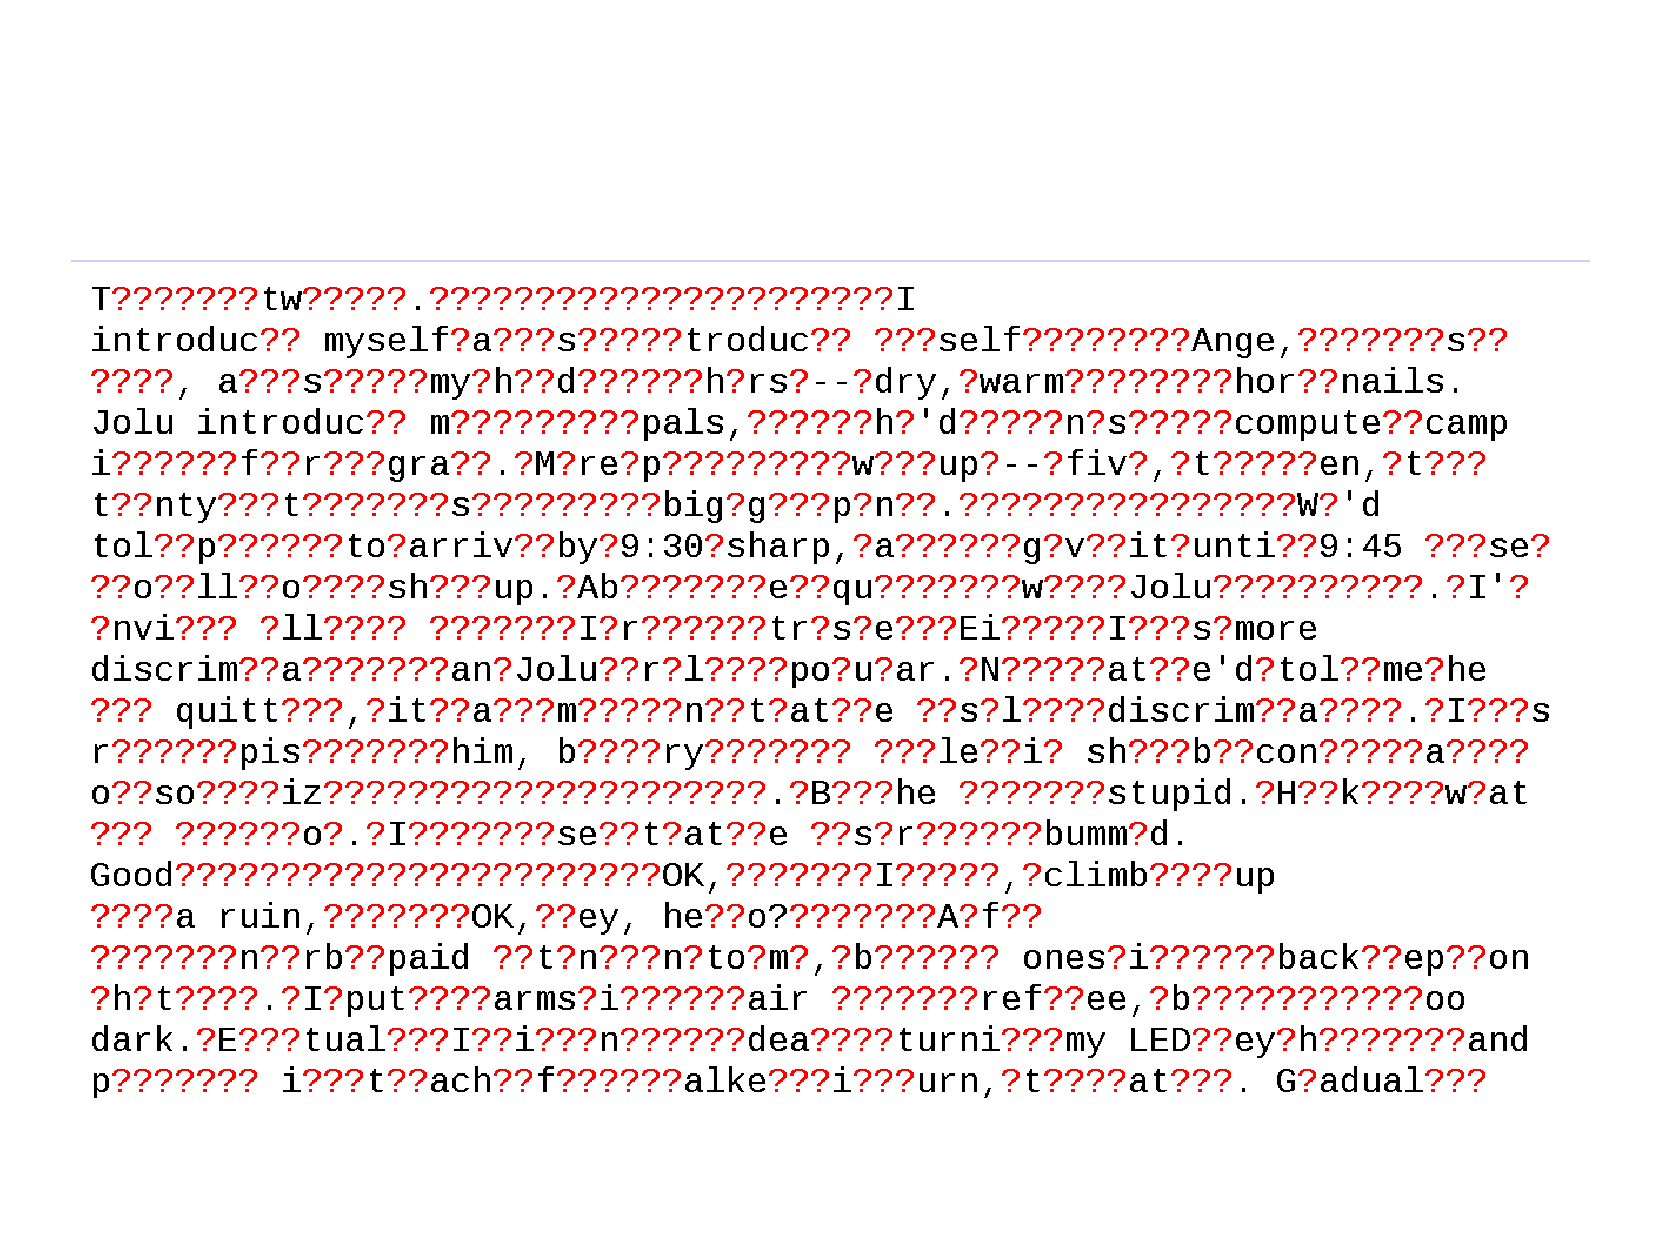
\includegraphics[width=3in]{art/brown-1} &  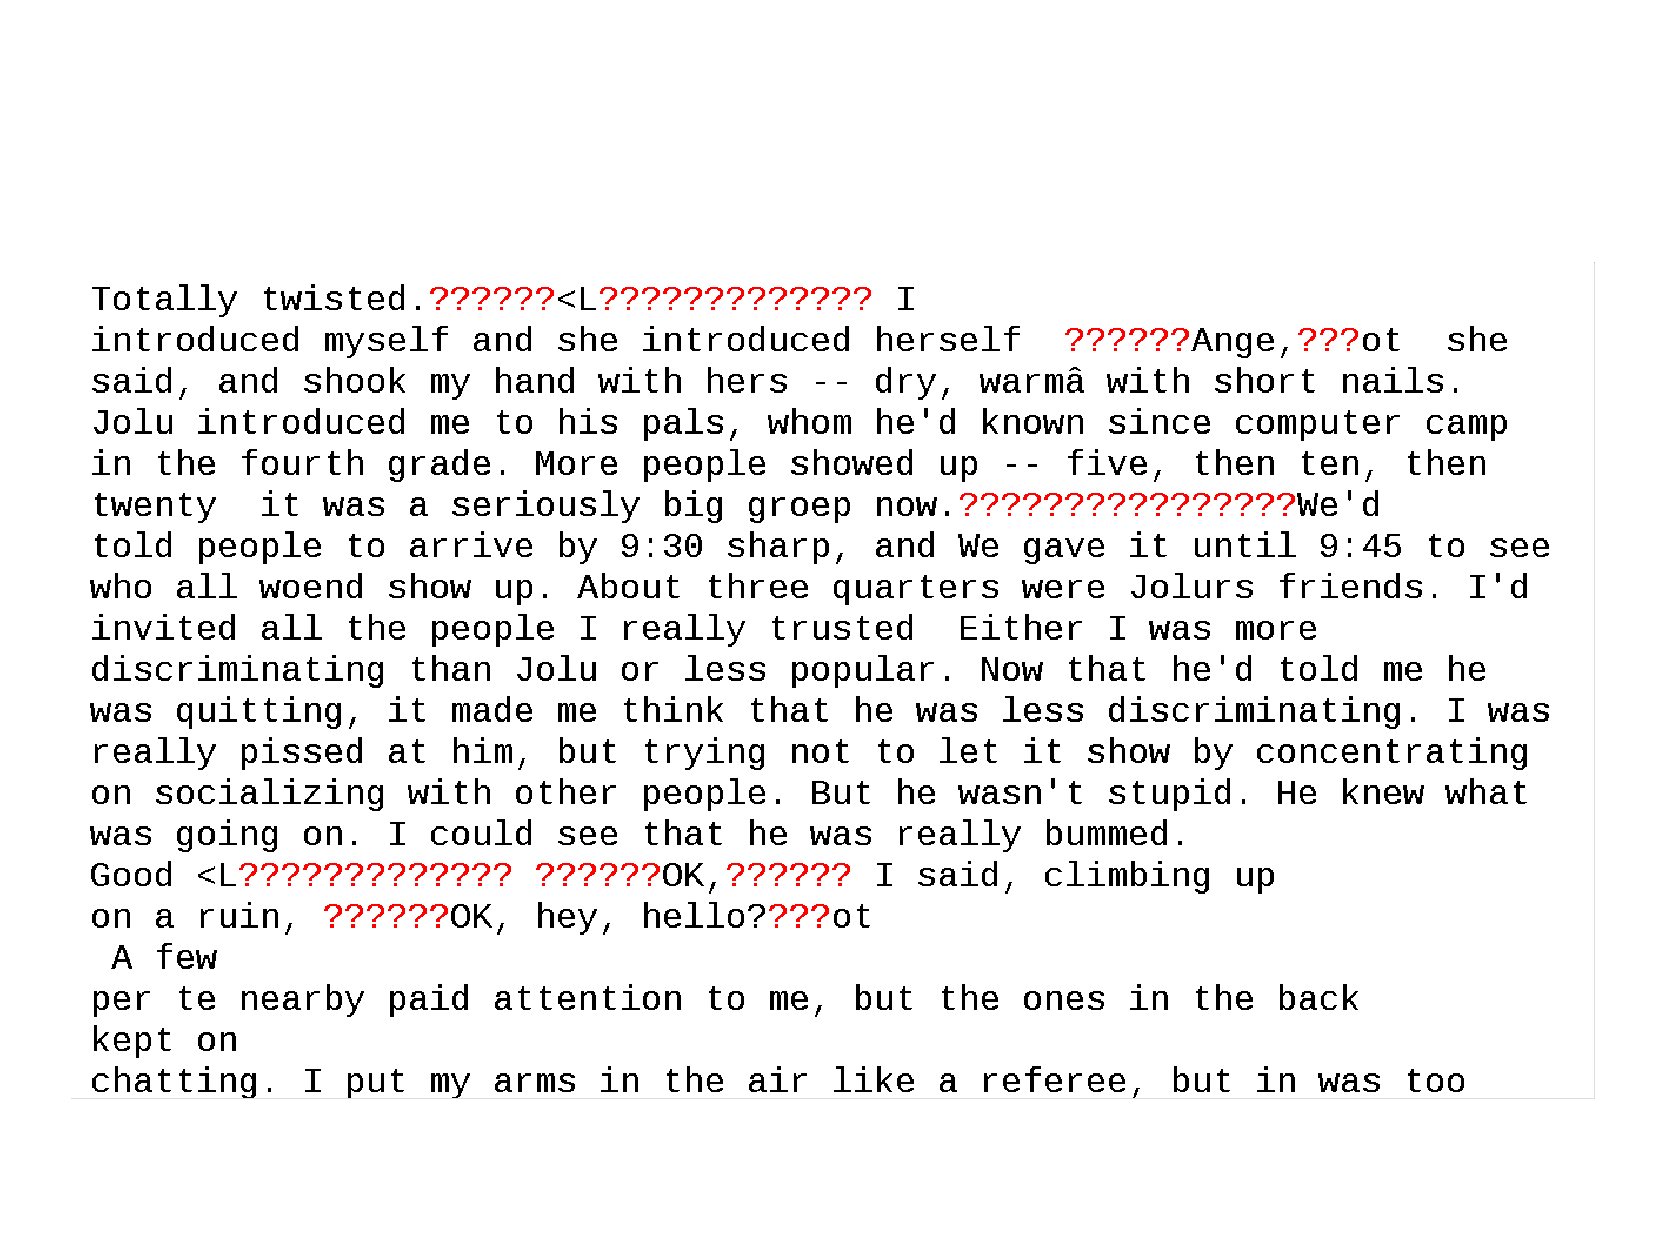
\includegraphics[width=3in]{art/brown-2} \\
\caption{Reconstructed text, without language model}\label{brown-1}
& \caption{Best possible reconstructed text, with language model}\label{brown-2}\\
\hline
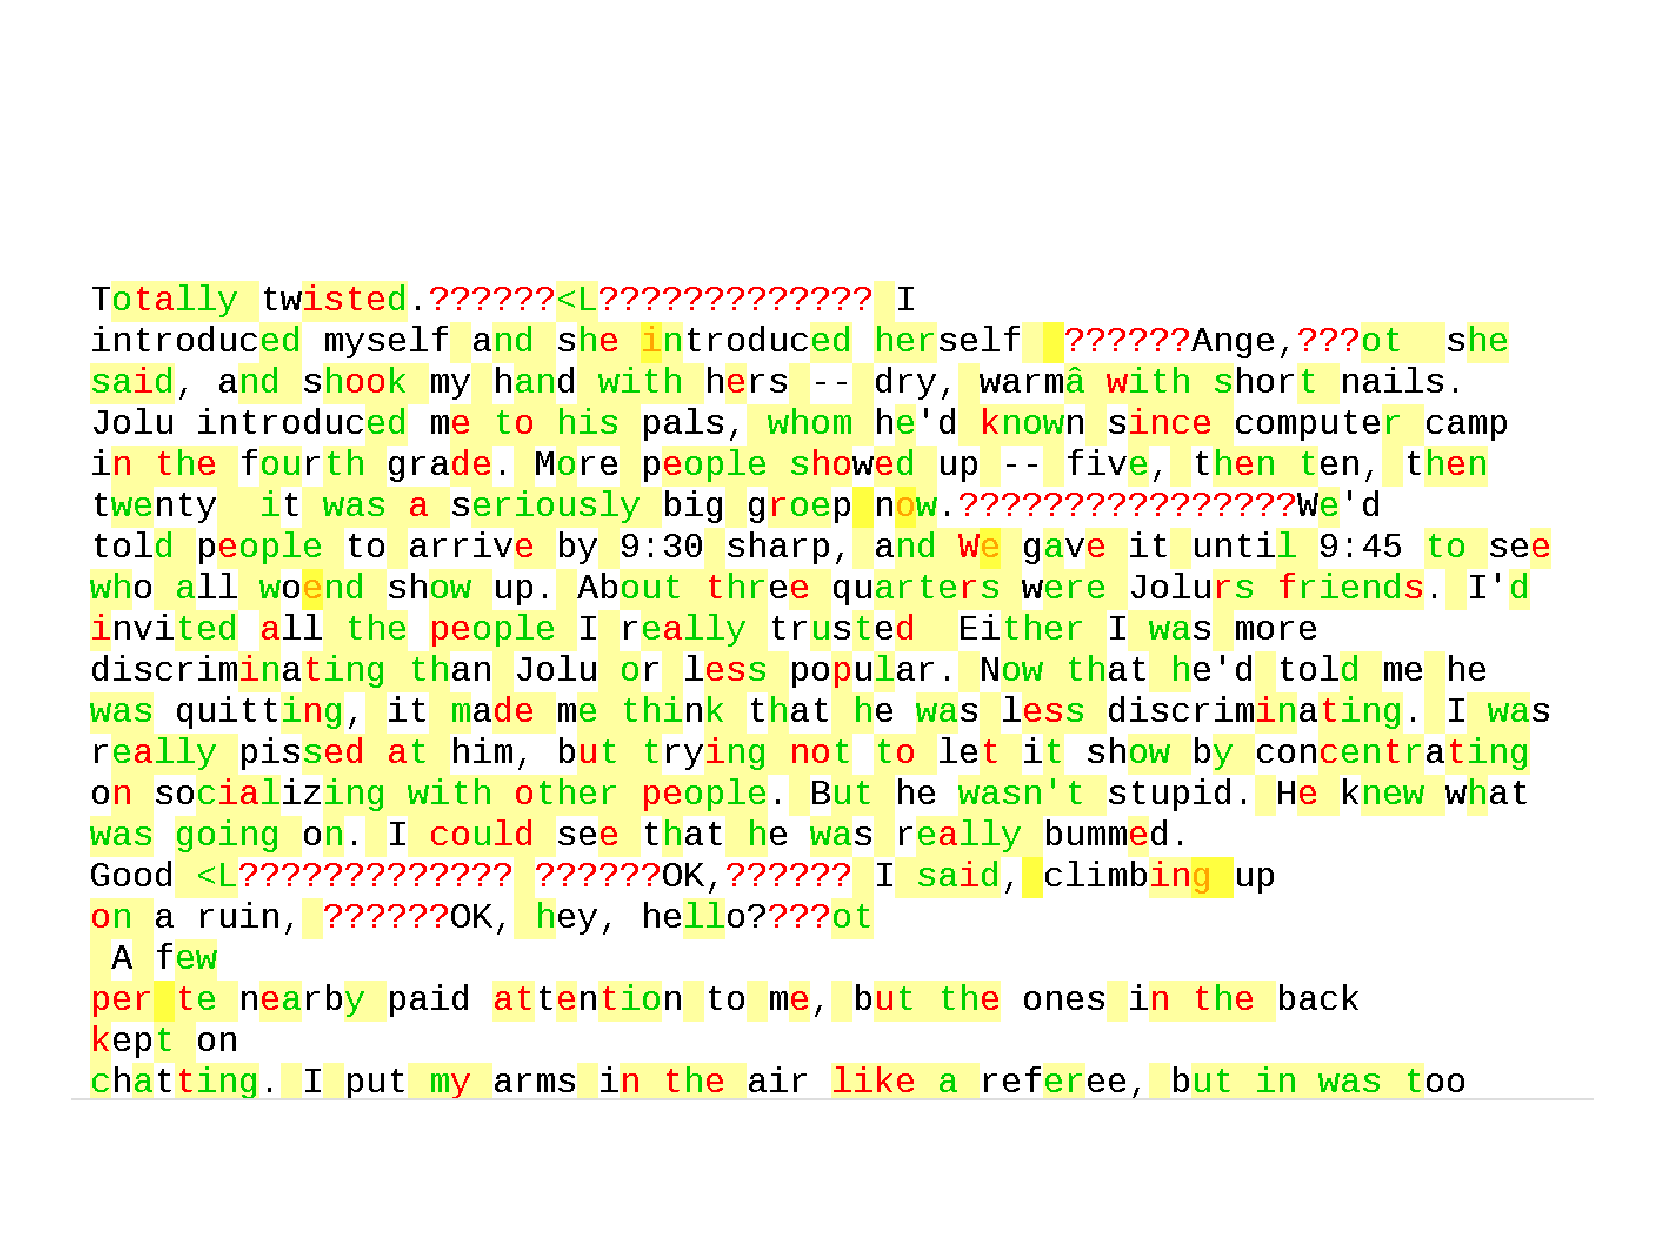
\includegraphics[width=3in]{art/brown-3} & 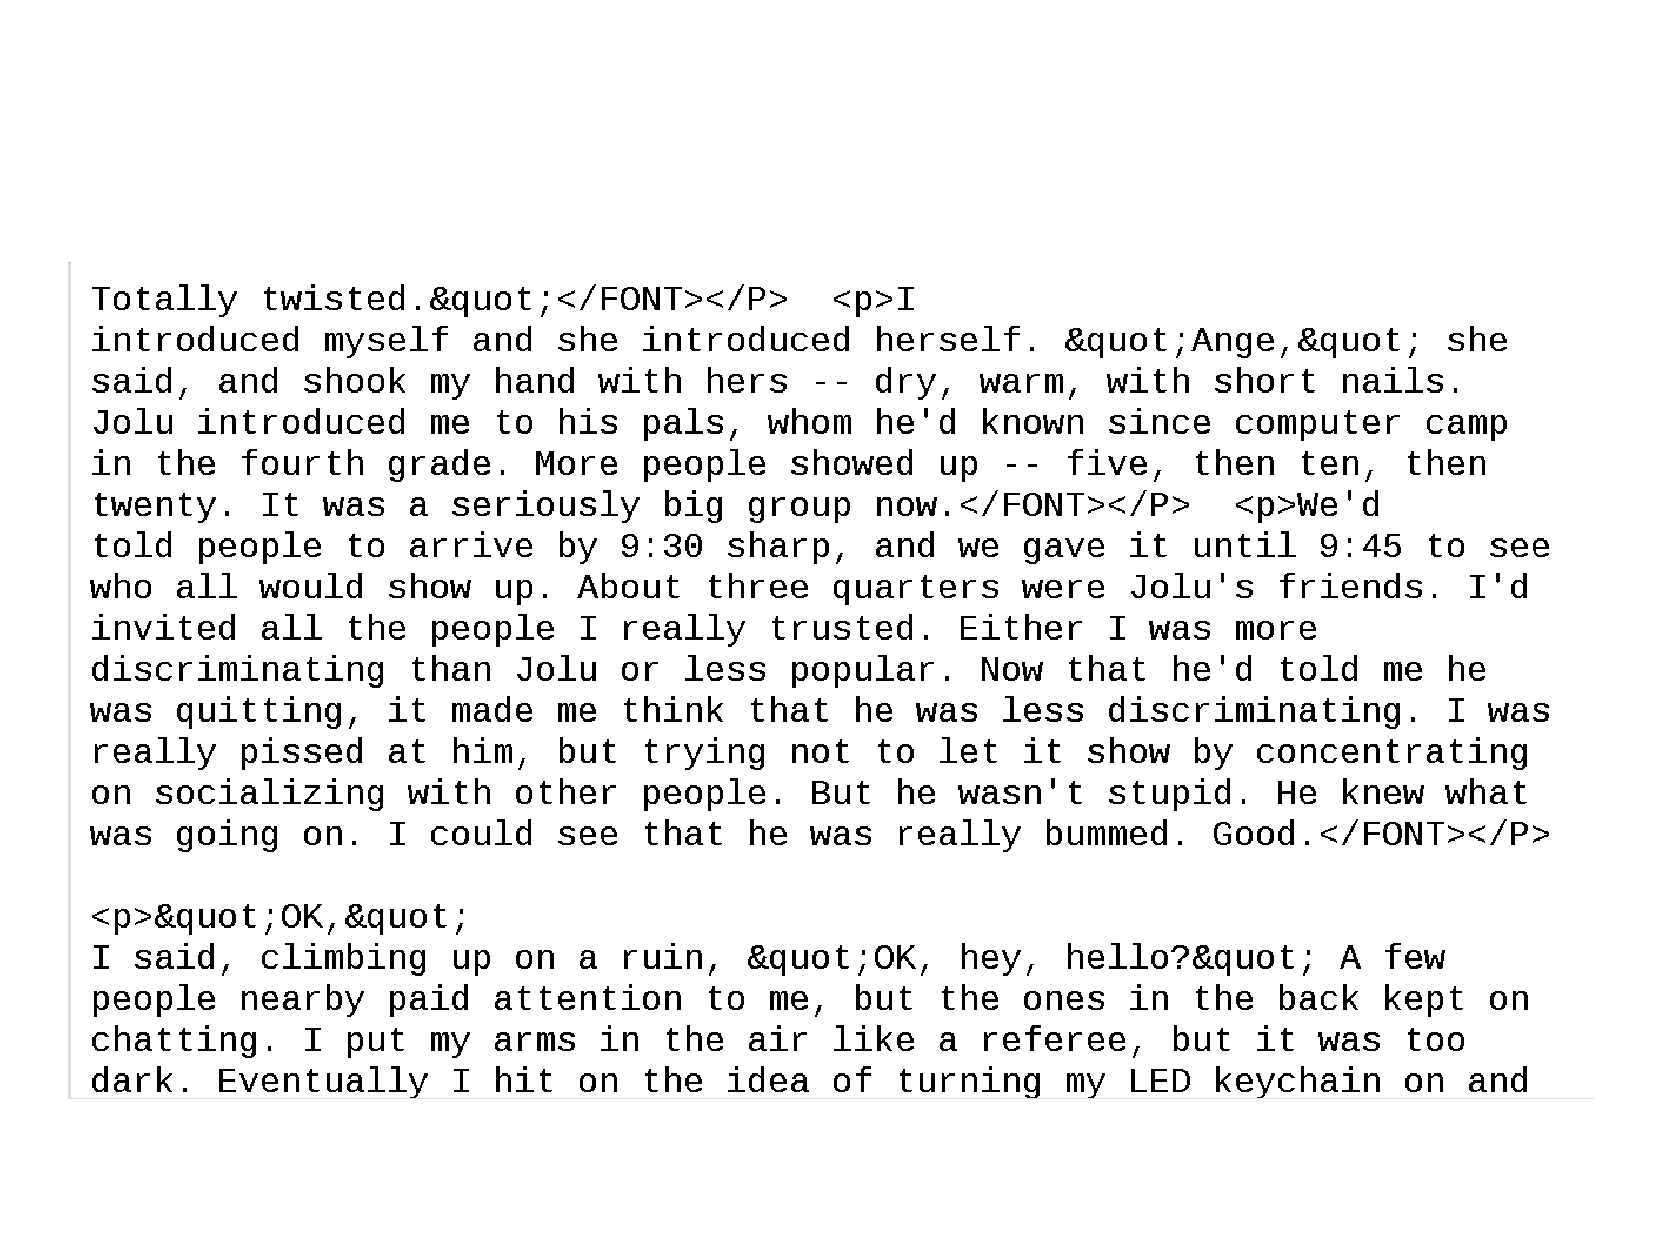
\includegraphics[width=3in]{art/brown-4}\\
\caption{Best possible reconstructed text, with language model. Green
  letters indicate high-probability matches, red letters indicate
  low-probability matches.}\label{brown-3}
&
\caption{Original text, from HTML version of Cory Doctorow novel
  ``Little Brother'', compressed using Info-Zip version 3.0, first
  1024 bytes of archive removed}\label{brown-4}
\\
\hline
\end{tabular}
\end{figure}


\subsection{Memory Parsing}

The memory of a desktop, laptop or cell phone is a mosaic of 4096-byte
blocks that variously 
contain running program code,  fragments of programs
that recently ran and have exited, portions of the computer's
operating system, fragments of what was sent and received over the
network, fragments of windows displayed on the computer's screen, the
computer's copy-and-paste buffer, and other kinds of information. Memory
changes rapidly---typical memory systems support several billion
changes per second---so it is nearly impossible to make a copy that is
internally consistent without halting the machine. An added complication is that the very
specific manner that programs store information in memory is rarely
documented and changes between one version of a program and
another. As a result, each version may need to be painstakingly reverse-engineered by
computer forensics researchers. Thus, memory analysis is time consuming, very
difficult, and necessarily incomplete.

Despite these challenges, recent years has seen the development of
forensically sound techniques for acquiring and analyzing the contents
of a running computer system. Today there are both open source and
proprietary memory analysis tools. These tools can take a memory dump
and report the system time when the memory was captured, display a
list of running processes, open files, and even display the contents
of the computer's clipboard and screen. Today memory analysis tools
are widely used for reverse-engineering computer viruses, worms and
other kinds of \emph{malware}, as well as for understanding an
attacker's actions in computer intrusion cases. Memory analysis can be combined
with carving to recover digital photographs and video.

\subsection{Fraud Detection in Multimedia}

Even when photos and video can be recovered from a subject's computer
or cell phone, another question to consider is whether or not the
imagery is real. Photographs were doctored long before the advent of
PhotoShop. For example, after he was purged by Stalin, Abel
Yenukidze was carefully removed from official photographs through a
series of skillful manipulations of light and negatives in a Kremlin darkroom\citet{stalins-darkroom}. Today
computer animation takes such manipulation to a completely new level,
with computers now able to synthesize scenes that are 
indistinguishable from recorded reality (\figref{ultra-realistic}). 

\begin{figure}
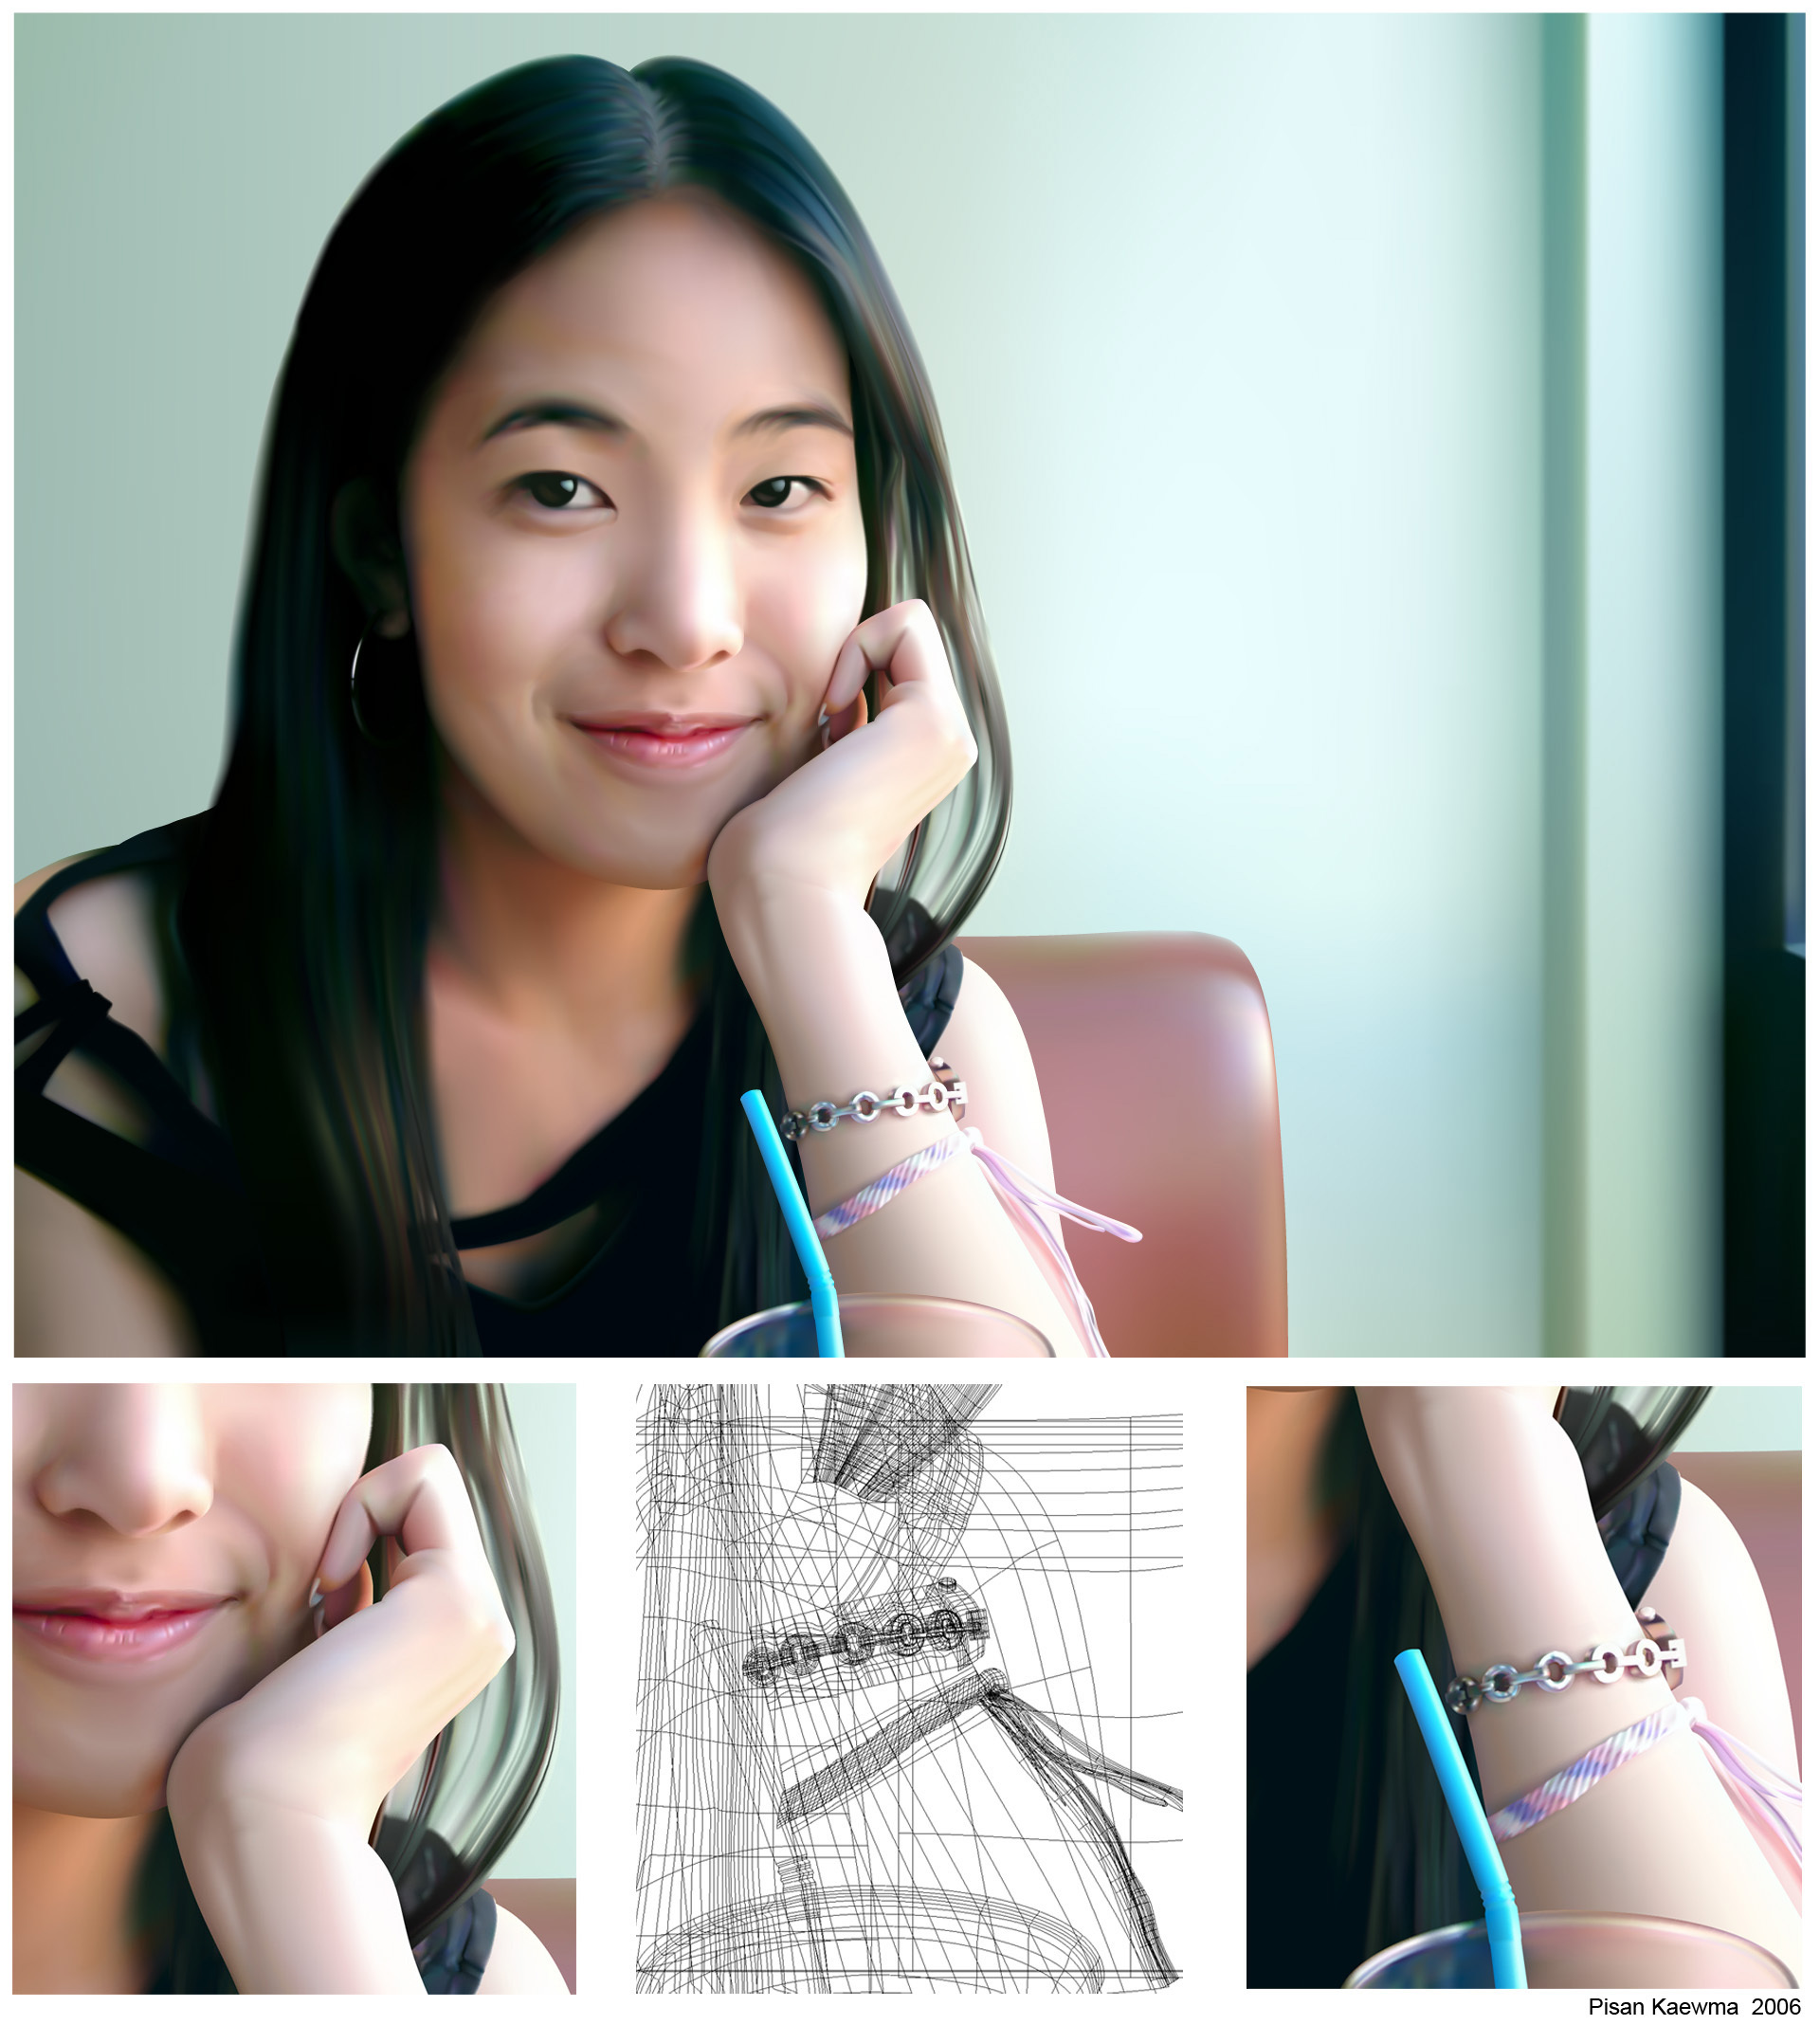
\includegraphics[width=4in]{art/a1336.jpg}
\caption{Ultra realistic vector gradient mesh using Adobe Illustrator by Pisan Kaewma, Thailand}\label{ultra-realistic}
% http://10steps.sg/inspirations/artworks/photo-realistic-vectors/
% http://www.ebypaidrick.com/Gallery.html
% http://www.illustratorworld.com/artwork/1336/
% http://rcpopart.com/labels/hyper-realist%20sculptor.html
% http://www.real-trace.com/index.html
\end{figure}

Recent developments in image processing have made it
possible to find some kinds of artifacts that indicate tampering or wholesale synthesis. For example,
the JPEG compression algorithm produces a mathematical signature when an
image is decompressed, cropped, and then re-compressed. Specular 
reflection, highlights and shadows can be closely examined to reveal
that different objects in a single ``photograph'' actually were
assembled from objects that were in 
slightly different physical environments. In one particular dramatic
demonstration, Dr.\ Hany Farid of Dartmouth University showed that a single ``group picture''
had been created by pasting in the people from different photos
because the reflection of the room lights on each person's eyeballs
were inconsistent with were they were standing in the frame. The technology is now
being commercialized\citep{farid07}.


\subsection{Automated Reasoning}

The leading edge of DF research are systems that
attempt to assist or even automate an analysts' reasoning---systems
that can automatically find evidence that is out of the ordinary,
strange, or inconsistent. Such details can indicate that there is a
deeper, hidden story. Inconsistencies can also indicate that evidence has been
tampered or entirely falsified. 

Ultimately, such automated reasoning systems are likely the only way
that today's analysts will be able to address the vast data
quantities and increasing diversity that they are likely to encounter
in the coming years. There has been some work in this area in
terms of systems that can find timestamp inconsistencies (a file
can't be deleted before it is created), but such rules are invariably
complicated by the messiness of the real world (for example, daylight
savings time). 

\section{The Digital Forensics Challenge}

For all of its power, DF practitioners face stark
challenges in practicing their discipline---challenges likely to
increase in the coming years. Those challenges are size,
time, diversity, cloud computing, encryption and language.

\begin{compactdesc}

\item[Size:] The past three decades have seen a steady increase in the
  amount of storage available to consumers and a steady decline in its
  cost. In 1993 I purchased my first 1 gigabyte external hard drive
  for a thousand dollars; today a 1 terabyte external hard drive can
  be purchased for under a hundred---a thousand times more
  storage for a tenth the price. Not surprisingly, the amount of data
  acquired by law enforcement organizations in their cases is
  increasing every year.

  Alarmingly, other aspects of computing have not scaled as quickly as
  storage. Today's terabyte drives are only 10 to 100 times faster
  than the gigabyte drives of yesteryear, which means that it takes anywhere
  from 10 to 100 times longer to copy  data from the larger
  drives. Likewise, today's computers are only on average 100 fold
  faster than the high-end workstations of the early 1990s, which
  means that there is less computing power available to process each
  byte per unit time. The continuation of these trends means that new techniques are
  required to deal with the data onslaught, as existing techniques
  simply cannot keep up with the increased storage available to consumers.

% My 33Mhz NeXTstation had 10 SPECmarks
% http://www.kevra.org/TheBestOfNext/NeXTProducts/NeXTHardware/NeXTStnColor/files/page620_2.pdf
% Intel Core i7 is 965 SPECmarks
% http://openlab.web.cern.ch/sites/openlab.web.cern.ch/files/technical_documents/CERN_openlab_report-Eval-of-energy-consumption-and-perf-of-Intel's-Nehalem-achitecture.pdf

\item[Time:] Even as the amount of storage received by law enforcement
  organizations increases, the time available to analyze that storage
  is steadily decreasing. In part this is because the number of cases
  in which digital evidence is collected is increasing far faster than
  the number of forensic investigators available to do the
  examinations. But another cause is the increasing realization that
  DF can be used to \emph{solve crimes}---that is, as
  part of the investigation process---whereas in the
  past DF was mainly a tool for \emph{assisting in convictions}. The
  shortened time horizons puts increased demands on tools,
  investigators, and systems.

\item[Diversity:] Forensic investigators must be able to process any
  information found on any computer system currently in use. After
  all, if there were a particular kind of system that could not be
  analyzed, criminals would be sure to use it. Thus, DF tools and
  invesitgators must be able to accommodate all kinds of computers,
  operating systems, application programs and the like. The diversity
  is particularly problematic in the case of cell phones, where there
  are literally dozens of different kinds of cables and tens of
  thousands of apps in widespread use that might require analysis.

\item[Cloud Computing:] Further complicating the investigator's job is
  the emergence of cloud computing and other technologies for storing
  data in the Internet rather than on desktops, laptops, and mobile
  devices. As a result of the cloud, there is no way to assure that a
  seized cell phone actually holds the suspect's data---the phone
  might simply be a tool for accessing a remote server. A law
  enforcement professional who is authorized to search a device may
  not have legal authority to use information on that device to access
  remotely stored data. Worse still, the data might be deleted in the
  meantime by one of the suspect's collaborators.

\item[Encryption:] The increased use of encryption means that
  investigators might not be able to decipher information once they
  have it in their possession. 

\item[Language:] Finally, in today's global environment forensics
  examiners are increasingly encountering evidence written in human
  languages that the examiner does not understand. And while tools
  like Systrans and Google Language Tools can perform some automated
  language translation, such systems are rarely sufficient for
  real-world forensic media.

\end{compactdesc}

These challenges impact the entire forensic processing model. Here are
two  examples:

\begin{compactitem}
\item Ten years ago it was relatively easy to collect and preserve a
computerized evidence: standard procedure was for law enforcement to
turn off a suspect's computer and take it back to the police station
where it might be put in an evidence locker. But modern computer systems
frequently employ encryption: turning them off may cause a key to be
erased, eliminating the possibility of decrypting the data without the
suspect's cooperation. For these systems it is now common practice to
copy out the computer's memory if possible---except that it is not
always possible because of diversity. 

\item Cell phones may be equipped with ``self destruct'' applications
  that wipe their data if they receive a particular text, so it is now
  standard practice to store phones in a shielded metal box called a
  Faraday cage that blocks radio waves. But many cell phones forget
  their storage if left off for too long, so the Faraday cages must be
  equipped with power strips and cell phone chargers.  Because many
  low-end cell phones have proprietary plugs, police must seize chargers as well.
\end{compactitem}


\subsection{The Research Agenda}

  Addressing these increases has only been possible through the
  collective research of government agencies, academics, and
  independent practitioners. These research efforts largely fall into
  three areas:

\begin{description}
\item[Reverse Engineering] has traditionally been the most basic form
  of DF research. Developers generally do not provide the public
  with details of how their systems work. This is obviously true of
  malware developers, but it is also true of legitimate companies that
  develop hardware and software, and even many open source
  systems. As a result, forensic practitioners must expend
  considerable effort reverse engineering systems to  understand how
  they work.  Today's techniques to extract allocated files from disk
  images were largely developed through reverse engineering.

\item[System Analysis] is the second leg of forensic research. System
  analysis is the systematic exploration of digital systems to
  understand the information that they contain and how it can be
  exploited for forensic analysis. Although similar to reverse
  engineering, system analysis is fundamentally different, in that the
  information the system analyst seeks may be unknown to the
  developers themselves. Although this may seem strange, remember that
  computers are vastly complicated systems: just as programmers
  frequently put bugs in their programs without realizing it, programs
  invariably have other behaviors that aren't bugs but are equally
  unforeseen by the original programmers. Many system users and quite
  a few developers assumed that it was not possible to recover deleted
  files until data recovery experts developed tools that proved otherwise.

 As long as there is data data that exists but which cannot be viewed
 through the operating system, there is need for tools that can
 display it. There is simply no commercial reason for software vendors
 to create tools which make this information visible---in many cases
 they are not even aware that the data is present. For example,
 previous versions of Microsoft Word left text in a
 document file even after it was deleted because the software didn't
 explicitly wipe the memory and corresponding disk sectors that
 corresponded to each deletion. This deleted-but-recoverable text
 occasionally resulted in some embarrassing revelations---so much, in
 fact, that many Microsoft products now explicitly have commands for
 to ``remove hidden data.'' Computer forensics tools can be
 used to both demonstrate the problem and verify whether or not
 Microsoft's solution actually works.

\item[Advances in fundamental science and engineering] are also needed
  for advances in DF. In particular, today's DF researchers are at the
  forefront of many other hot fields in computer science, including
  cloud computing, big data, visualization, and natural language
  processing. File carving and the recovery of data from corrupted
  compressed files are both examples of this kind of work: much of
  this work was thought to be computationally prohibitive until new
  mathematical algorithms were developed that proved
  otherwise. Another example is software that automatically translates
  posts on Facebook and Twitter from the subject's native tongue into
  a human language that the examiner can understand.
\end{description}


\subsection{Human Capital}

\textbf{Insert training prior art.}



\chapter{Handling Digital Evidence}
The fundamental nature of digital information makes the practice of
digital forensics fundamentally different from other kinds of forensic
processes.  Whereas forensic scientists may have just a few drops of
blood or a few bullet fragments with which to work, digital data is
marked by its volume, the ease with which it may be copied, and the
ability to change it without a trace of the previous value.

Many mass storage systems have the some kind of \emph{hardware
  write-protect} that can be used to prevent accidental overwriting or
erasure. For example, 9-track tape features a
write-protection ring which, when removed, prevented the tape from
being written on, while $5\frac{1}{4}''$ floppy disks had notches cut into
the side that could be covered to inhibit writing. Early disk systems
also had hardware write-protect, but mass market hard drives that
became available in the mid 1980s did not have such a feature. As a
result, several approaches emerged to allow examination of digital
data while minimizing the chances of changing it: write
blockers, mirror drives, and forensic disk images.
% Poil - GFDL - 2005
% http://en.wikipedia.org/wiki/File:Tapeprotection.jpg

\section{Collecting and Preserving Stored Digital Evidence}

In computing the word \emph{store}
is used both as a verb (the act of storing the information) and a noun
(the place where the information is stored). Computer systems have two
kinds of storage systems:

\begin{description}
\item[Primary Storage] is storage that can be directly accessed by the
  computer's central processing unit (CPU). Most computers use
  \emph{Random Access Memory} (RAM) as their primary storage, although
  some systems can also use a special kind of flash memory called
  \emph{NOR Flash}. 

\item[Secondary Storage] is storage that cannot be directly accessed
  by the CPU. To use secondary storage, information must be copied
  between secondary storage and primary storage. Typically these copy
  operations are performed on fixed-sized \emph{blocks} of data.
\end{description}

Even though this chapter is concerned with data on mass
storage system, we will see that forensic containers need to be able
to store a wide variety of other kinds of information, including
network packets, memory dumps, and even individual files. These
additional modalities are required for a variety of reasons:


\subsection{Write Blockers}

Removable media such as floppy disks, tapes and storage cartridges
used in the 1990s generally had some kind of \emph{write-protect}
switch or tab that could be used to prevent inadvertant alternation or
overwriting of evidence. Hard drives of the time had no such
facility. To overcome this deficiency the industry invented
\emph{write-blockers}, a device that can be inserted inline between a
hard drive and a computer system. A typical write blocker might have a
male and a female connector; the female connector plugs into
the hard drive's male connector, while the blocker's male
connector plugs into a cable that connects to the host computer.

Write blockers allow examination of subject data without fear of
inadvertently modifying the contents---provided that the write blocker
works properly. A problem with the concept of write blockers is that
the only real specification of what these devices should do was their
name---that is, they should block modification of data on the hard
drive.  

There are generally two design choices that must be decided when
creating a write blocker:

* Determining which commands are write commands.

* Determining what to do when write commands are executed.

But there
are two ways to do this. One is to literally block the commands that
alter data, a task that requires a clear enumeration of all such
commands. An alternative (and somewhat safer) strategy is to only pass
those commands that are known \emph{not} to alter
data\cite{dfrws2006:JamesLyle}. Both of these approaches
implicitly assume that the only way data is altered on the drive is
through the execution of commands, and this is not actually the
case. For example, the S.M.A.R.T. counters inside modern drives that
track the number of seconds the drive is powered up will continue to
advance even when a write-blocker is in place.


A write blocker can allow \emph{read} commands
to pass while immediately returning an error condition when a
\emph{write} command is attempted. Alternatively the \emph{write}
commands may be executed on a different piece of media, sometimes
called a \emph{shadow drive}, giving the operating system the
appearance of a successful write while leaving the original media
undamaged.


Write blockers can be used to allow an examiner to directly examine
subject data on the original media. Alternatively, they can be used to allow the subject
data to be safely copied to a second piece of media called a
\emph{mirror drive}. It is important that the mirror drive be
\emph{cleared} before the copy is made to assure that there is no
\emph{cross-case contamination}, which happens when data are
inappropriately mixed between cases. Clearing is especially important
if the subject drive has errors or if the mirror drive is larger than
the subject drive.



\subsection{Disk Imagers}

The copy from the subject drive to the mirror drive is performed with
a program called a \emph{disk imager}.

\section{Image Files}

\citeN{dfrws2002:JamesLyle} introduced the Computer Forensic Tool Testing (CFTT)
program at the National Institute of Standards and Technology (NIST).



Instead of making a copy to a mirror disk, it is possible to copy all
of the accessible blocks on a mass storage system into a single file
on a computer disk. Such files are called \emph{image files} because
they represent an image of the information stored on the disk. The
term ``image'' here should not be confused with the other usage of the
word ``image'' to describe a photograph.

A raw disk image is a byte-for-byte copy of a mass storage
system. Such files can be quite large---a 256GB drive will have a raw
image that is 256GB in size. This can cause problems, as many computer
systems cannot operate on files that are larger than 2GiB or 4GiB due
to 32-bit limitations. One way to address the file size limitation is
by splitting the file into multiple files of equal size---for example,
a 256GB disk image can be split into 256 files of 1GB each. Such
collections of files are called \emph{split raw images}; each file is
typically given a name such as \emph{FILENAME.000}, \emph{FILENAME.001},
\emph{FILENAME.002} and so on.

A second and more important problem with raw image files is that they
lack important \emph{metadata} about the process by which they were
acquired. Metadata is data about data; in the case of files in a file
system the metadata includes the file's name, timestamps, and other
kinds of file system information. But in the case of disk images,
there is a wealth of additional metadata that can be collected, such
as:

\begin{itemize}
\item The date and time that the disk was imaged.
\item The manufacturer, model number, and serial number of the disk
  that was imaged.
\item The examiner that did the imaging.
\item The physical location where the image was made.
\item Other notes about the imaging process or the physical artifact.
\end{itemize}

There is also need for integrity controls to assure that the disk was
properly imaged and that the image itself was not altered or corrupted
after the file was created. A common integrity control is to compute
the cryptograhpic hash of the disk image's bitstream, computed by
feeding all of the bytes in the disk image into a hash function such
as MD5 or SHA1. Cryptographic hashes have the property that changing a
single bit causes the resulting hash function to change
unpredictably. In practice, the examiner computes the hash of the disk
image and stores this information separately---for example, by writing
it in a notebook. The disk can then be imaged a second time. If the
two disk images have the same hash, then the examiner can assume that
the image itself is a faithful copy of the source disk. Later, the
examiner can re-calculate the hash of the disk image to show that the
image has not been modified.

Compression can significantly shrink the size of a disk image
file. Although it is tempting to such programs such as ZIP and GZIP
directly on a raw file, the resulting file must be entirely
decompressed before it can be used. For files larger than a gigabyte
this quickly proves unworkable. Instead, it is common practice to
use a file format that breaks the raw disk image into blocks or
segments and compresses each individually. These segments are then
stored in the resulting image file, along with some kind of map that
describes, for each segment, the offset within the original uncompressed file
and the physical offset of the compressed segment in the compressed file.

[Diagram showing the original file, the compressed file, and the map]

\subsection{Image File Formats}
Today a wide number of image file formats are in use. Broadly
speaking, there are formats that were developed for digital forensics
and those developed for mainstream computing. Within the set of
formats developed for digital forensics, there are \emph{proprietary formats} that were developed by
vendors for commercial tools and \emph{open source} formats that were
largely developed for academic purposes. However the distinction can
be misleading, as there exists several open source implementations for
the proprietary formats, making them somewhat open source. 

\subsubsection{Proprietary Forensic Formats}

SafeBack~\cite{safeback}, a DOS-based utility designed to create
exact copies of entire disks or partitions, offers a
``self-authenticating'' format for images, whereby SHA256 hashes are
stored along with data to ensure the latter's integrity.  Although
few technical details are disclosed publicly, SafeBack's authors
claim that the software ``safeguards the internally stored SHA256
values''~\cite{safebacksafeguards}.


The most widely disk image format appears to be Guidance Software's EnCase Forensic~\cite{encase} uses
a proprietary format for images, reportedly based on ASR Data's
Expert Witness Compression Format~\cite{ew}.  EnCase's Evidence File
(.E01) format~(Fig.~\ref{fig:encase}) contains a physical bitstream
of an acquired disk, prefixed with a ``Case Info'' header,
interlaced with CRCs for every block of 64 sectors~(32 KB), and
followed by a footer containing an MD5 hash for the entire
bitstream.  Contained in the header are the date and time of
acquisition, an examiner's name, notes on the acquisition, and an
optional password; the header concludes with its own CRC. 

The E01 format allows for the contents of a disk image to be
compressed. Each image volume contains a so-called ``jump table'' that
contains the offset of each block in the original uncompressed disk,
the offset in the disk image of the compressed block, and the size of
the compressed block. Originally offsets were described with 32-bit
signed integers, limiting the size of the disk image volume to 2GiB;
additional volume files with extensions E02, E03, and so on could be
added to create images of disks that could not fit within a single
volume. The EnCase imager allows the user to specify a maximum size
for each of these files: setting the size to 700MB allows each volume
to be burned to a CD-R. 

AccessData's Forensic Toolkit (FTK)
supports storage of disk images in EnCase's or SMART's file format,
as well as in raw format and an older version of Safeback's format
(Section~\ref{sec:safeback}). 

\subsection{ILook Investigator's IDIF, IRBF, and IEIF Formats}
ILook Investigator v8~\cite{ILookv8} and its disk-imaging
counterpart, IXimager, offer three proprietary, authenticated image
formats: compressed (IDIF), non-compressed (IRBF), and encrypted
(IEIF). Although few technical details are disclosed publicly,
IXimager's online documentation~\cite{IXimager} provides some
insights:  IDIF ``includes protective mechanisms to detect changes
from the source image entity to the output form'' and supports
``logging of user actions within the confines of that event;''  IRBF
is similar to IDIF except that disk images are left uncompressed;
IEIF, meanwhile, encrypts said images.

For compatibility with ILook Investigator v7 and other forensic
tools, IXimager allows for the transformation of each of these
formats into raw format.

\subsection{ProDiscover Family's ProDiscover Image File Format}
Used by Technology Pathways' ProDiscover Family of security tools
\cite{prodiscover}, the ProDiscover Image File format
\cite{prodiscoverformat} consists of five parts: a 16-byte Image
File Header, which includes a signature and version number for an
image; a 681-byte Image Data Header, which contains user-provided
metadata about the image; Image Data, which comprises a single block
of uncompressed data or an array of blocks of compressed data; an
Array of Compressed Blocks sizes (if the Image Data is, in fact,
compressed); and I/O Log Errors describing any problems during the
image's acquisition.

Though well documented, the format is not extensible.


\subsubsection{Open Source Forensic Formats}

Supported by PyFlag\footnote{In addition to its own {\tt sgzip} format,
PyFlag can also read and write the Expert Witness Compression Format
\cite{pyflagiosources}.}~\cite{pyflag}, a ``Forensic and Log
Analysis GUI'' begun as a project in the Australian Department of
Defence, {\tt sgzip} is a seekable variant of the {\tt gzip} format.  By
compressing blocks (of 32KB, by default) individually, {\tt sgzip} allows
for rapid accessing of the disk image by forensic software without the
need to first decompress the entire image. The format does not associate metadata with images.
\cite{pyflagdiskforensics,pyflagiosources}



\citeN{dfrws2005:PhilipTurner} introduced \emph{digital evidence bags}
as a way of supporting \emph{selective imaging}. Turner's file format
is similar to EnCase's L01 format in that it supports logical files in
addition to physical sectors.



\subsection{Digital Evidence Containers}

Mirror copies can be unwieldy to use, especially when the target
drives are very large. An added annoyance is that many drives contain
a large number of highly compressible data, such as sectors filled
with NULLs. Yet another problem is that there is no easy way to tell
if the copy is accurate or if the copy has been modified after it was
originally made.

\emph{Digital evidence containers} allow for digital evidence to be
copied into an archive that is \emph{compressed} (to allow for easier
data handling), \emph{integrity checked} (so that the examiner can
verify the original data), \emph{annotated} with metadata such as the
time that the evidence was copied, the name of the investigator who
created the archive, the location where the copy was made, and other
similar information. Unlike ZIP or gzip files, these containers must
also allow for \emph{random access} their contents, as it would not be
efficient to decompress a multi-gigabyte data stream for the purpose
of accessing just a few sectors.

Additional requirements include \emph{Encryption}, so that access to
the evidence can be restricted to those that have a password or
decryption key; metadata specifically devoted to
\emph{chain-of-custody} and \emph{provenance}, so that the movement of
evidence through an organization or a forensic pipeline can be
electronically recorded; and \emph{external references}, so that the
evidence container can point to information present on other storage
systems.

\subsection{Other Kinds of Digital Evidence}

* Cell phones

* Memory

* Network Evidence

\begin{itemize}
\item Data from networks or memory is frequently found on subject hard
  drives. When it is found, it is useful for the forensic examiner to
  extract that data and store it in its own container. 
\end{itemize}


\section{File System Analysis and File Extraction}

\subsection{Files and File Systems}
The word \emph{file} is commonly used to describe a sequence of data
that is stored on a computer mass storage system. On modern computers
files are sequences of zero or more \emph{bytes}. Files have a length
that is set at any given point in time, but can be readily
changed. Files can have names and other associated \emph{metadata}
such as timestamps, an owner, and a group. Files have traditionally
been grouped together in
\emph{directories}\wikipedia{http://en.wikipedia.org/wiki/File_directory}. also
called \emph{folders}.

The phrase \emph{File
  System}\wikipedia{http://en.wikipedia.org/wiki/Computer_file} is
used to describe the part of the computer's operating system that
manages a storage system. However, the term is also used to describe
the very sectors on a mass storage device that contain the files.

It is important to realize that files are an \emph{abstraction} that
was created for the purpose of managing data. There is nothing
inherent in the design of computers, operating systems or mass storage
devices that requires the use of files. A raw disk can be used as
virtual memory \emph{backing store} or as a storage system for a
database. Instead of stored as a sequence of bytes in a file, data can be stored as
objects that are persisted in memory, or as BLOBs in a database.

It is also important to realize that any computational storage device
or abstraction can be used to virtualize and contain any other storage
device. That is, a file can be stored in a file system, but a file
system can also be created and stored inside a file (this is
essentially what a disk image is). Most operating systems can swap to raw
partitions or to files, but file systems can also be created inside
RAM or virtual memory.

Adding to the complexity of the forensic examiner is
\emph{encryption}, which can be applied at the interface between any
of these abstractions. Encryption can be performed in the storage
device itself (as in the case of an encrypting hard drive), in the
disk driver, in the logical volume management system, in the file
system, or at the application level.

\subsection{File Systems of Forensic Interest}
There are a variety of different kinds of file systems in use on
modern computer systems:
\begin{description}
\item[Disk file systems] organize files and directories on
  block-oriented storage systems. These are of interest to those
  engaged in MEDEX operations. Popular file systems include FAT32
  (used primary on removable storage devices and camera cards), NTFS
  (Microsoft's New Technology File System), and HFS+ (Apple's
  Hierarchical File System used on Macs and iPhones).
\item[Distributed file systems] allow a computer to access
  information on remote servers as if it is stored
  locally. Distributed file systems are forensically interesting
  because many use local storage to cache information from the remote
  servers. Analyzing local storage can therefore give clues as to what
  was accessed remotely, and when it was accessed.
\item[Virtual file systems] use the file and directory abstraction to
  make it easy to access other information. For example, the Linux
  \url{/dev} file system is used to access devices through the file
  system, the \url{/sys} file system is used to access features within
  the system kernel, and the \url{/net} file system accesses the
  automounter. Virtual file systems are not typically of interest in
  MEDEX because they do not leave residual information on a storage
  device. However, virtual file systems are relevant in malware
  analysis and intrusion response.
\end{description}

As this survey is written, specific file systems of interest include:
\begin{description}
\item[FAT12, FAT16 and FAT32] file systems developed by Microsoft for use with
  DOS. FAT refers to the File Allocation Table, an array of integers
  that is used to determine if a cluster is in use or free. (In FAT, a
  \emph{cluster} is a block of 1, 2, 4, 8 or more disk sectors.) The number
  refers to the size of the integers in the array (12 bits, 16 bits or
  32 bits). Today implementations of FAT are built in to practically every
  operating system, including Windows, Linux, MacOS, most digital
  cameras, and practically every other device with a USB or SD
  interface. 
\item[NTFS] 
\item[HFS+]
\item[YAFFS2]
\item[EXT2/3]
\item[EXT4]
\end{description}

Information can be hidden in a file system by storing data in blocks
that are allocated but not used to hold content\cite{dfrws2005:KnutEcksteinAndMarkoJahnke}. 

\subsection{File System Structures and Terminology}

Blocks

Clusters

inode

Hard Link

Symbolic Link

Master File Table

File Allocation Table

Free List

Unlink

\subsection{Classification of file system information}

Allocated

Deleted

 - Recoverable through undeletion

 - Recoverable through carving

Partially overwritten

\subsection{SSDs and the ``TRIM'' command}
\cite{dfrws2011:TimothyVidasAndChengyeZhangAndNicolasChristin}


\section{File Deletion and Deleted File Recovery}\label{deleted_file_recovery}
Different file system implementations delete files in different ways.

Traditionally, file systems simply \emph{unlinked} files---the pointer
to the file was removed from the directory, and the blocks associated
with the file were returned to the free list.


\section{Exploiting File System Metadata}
File system metadata can be used to determine usage. 
\cite{dfrws2011:JonathanGrier}

% October 12
%\chapter{File System Analysis and File Extraction}

\sgraphic{art/filesystems}{Mass storage devices are typically used to
  hold one or more file systems. Disks start at Logical Block Address
  0. Legacy partitioning schemes such as Master Boot Record (MBR)
  start at LBA 0, while the GUID Partitioning Table (GPT) schem starts
  at LBA 1. In either case the partition table conveys the number of
  partitions and the address at which each one starts. There may be
  gaps between the partition map and the first file systems, and there
  may be gaps between the file systems. These gaps may be blank or may
  contain residual data from previous uses of the disk---ghost file
  systems from an early
  time.
}

In the previous chapter we discussed how data on a mass storage device
can be extracted and preserved. In this chapter we will begin the
analysis of data that has been successfully extracted from a mass
storage device.

\section{Background}
Although there are many ways to store information on a hard drive or
other mass storage device, most drives are used to store one or more
\emph{file systems}. These file systems, in turn, are used to store
named files which are themselves arranged in named directories. 

\subsection{Partitioning and Volume Management}

Although a file system can be stored directly on the drive, with the
file sector of the drive being used to store the first sector of the
file system, this is not commonly done. Instead, the first 1 or 2
sectors are used for a \emph{partition table} that describes the
locations of the file systems. In this way a single device can be used
to simulate multiple logical devices. Two commonly used partitioning
schemes are the \emph{Master Boot Record} and the \emph{GUID Partition
  Table} scheme.\wikipedia{http://en.wikipedia.org/wiki/GUID_Partition_Table}
       \wikipediab{http://en.wikipedia.org/wiki/Master_boot_record}

The term \emph{physical volume} is used variously to describe a
physical disk, a partition on a physical disk, or a Logical Unit
Number (LUN) of a storage
system.\wikipedia{http://en.wikipedia.org/wiki/Logical_Unit_Number}
Physical volumes can be used directly to hold a file system or can be
grouped together with a Logical Volume Management (LVM)
system\wikipedia{http://en.wikipedia.org/wiki/Logical_volume_management}. An
LVM can group multiple physical volumes together in to a single
physical volume that is large or more reliable than the volumes that
it built from. Volume managers can also implement
\emph{snapshots}\wikipedia{http://en.wikipedia.org/wiki/Snapshot_(computer_storage)}
through the use of
\emph{copy-on-write}\wikipedia{http://en.wikipedia.org/wiki/Copy-on-write}.

\subsection{Files and File Systems}
The word \emph{file} is commonly used to describe a sequence of data
that is stored on a computer mass storage system. On modern computers
files are sequences of zero or more \emph{bytes}. Files have a length
that is set at any given point in time, but can be readily
changed. Files can have names and other associated \emph{metadata}
such as timestamps, an owner, and a group. Files have traditionally
been grouped together in
\emph{directories}\wikipedia{http://en.wikipedia.org/wiki/File_directory}. also
called \emph{folders}. 

The phrase \emph{File
  System}\wikipedia{http://en.wikipedia.org/wiki/Computer_file} is
used to describe the part of the computer's operating
system that manages a storage system. However, the term is also used
to describe the very sectors on a mass storage device that contain the
files.

It is important to realize that files are an \emph{abstraction} that
was created for the purpose of managing data. There is nothing
inherent in the design of computers, operating systems or mass storage
devices that requires the use of files. A raw disk can be used as
virtual memory \emph{backing store} or as a storage system for a
database. Instead of stored as a sequence of bytes in a file, data can be stored as
objects that are persisted in memory, or as BLOBs in a database.

It is also important to realize that any computational storage device
or abstraction can be used to virtualize and contain any other storage
device. That is, a file can be stored in a file system, but a file
system can also be created and stored inside a file (this is
essentially what a disk image is). Most operating systems can swap to raw
partitions or to files, but file systems can also be created inside
RAM or virtual memory.

Adding to the complexity of the forensic examiner is
\emph{encryption}, which can be applied at the interface between any
of these abstractions. Encryption can be performed in the storage
device itself (as in the case of an encrypting hard drive), in the
disk driver, in the logical volume management system, in the file
system, or at the application level.

\subsection{File Systems of Forensic Interest}
There are a variety of different kinds of file systems in use on
modern computer systems:
\begin{description}
\item[Disk file systems] organize files and directories on
  block-oriented storage systems. These are of interest to those
  engaged in MEDEX operations. Popular file systems include FAT32
  (used primary on removable storage devices and camera cards), NTFS
  (Microsoft's New Technology File System), and HFS+ (Apple's
  Hierarchical File System used on Macs and iPhones).
\item[Distributed file systems] allow a computer to access
  information on remote servers as if it is stored
  locally. Distributed file systems are forensically interesting
  because many use local storage to cache information from the remote
  servers. Analyzing local storage can therefore give clues as to what
  was accessed remotely, and when it was accessed.
\item[Virtual file systems] use the file and directory abstraction to
  make it easy to access other information. For example, the Linux
  \url{/dev} file system is used to access devices through the file
  system, the \url{/sys} file system is used to access features within
  the system kernel, and the \url{/net} file system accesses the
  automounter. Virtual file systems are not typically of interest in
  MEDEX because they do not leave residual information on a storage
  device. However, virtual file systems are relevant in malware
  analysis and intrusion response.
\end{description}

As this chapter is written, specific file systems of interest include:
\begin{description}
\item[FAT12, FAT16 and FAT32] file systems developed by Microsoft for use with
  DOS. FAT refers to the File Allocation Table, an array of integers
  that is used to determine if a cluster is in use or free. (In FAT, a
  \emph{cluster} is a block of 1, 2, 4, 8 or more disk sectors.) The number
  refers to the size of the integers in the array (12 bits, 16 bits or
  32 bits). Today implementations of FAT are built in to practically every
  operating system, including Windows, Linux, MacOS, most digital
  cameras, and practically every other device with a USB or SD
  interface. 
\item[NTFS] 
\item[HFS+]
\item[YAFFS2]
\item[EXT2/3]
\item[EXT4]
\end{description}

Information can be hidden in a file system by storing data in blocks
that are allocated but not used to hold content\cite{dfrws2005:KnutEcksteinAndMarkoJahnke}. 

\subsection{File System Structures and Terminology}

Blocks

Clusters

inode

Hard Link

Symbolic Link

Master File Table

File Allocation Table

Free List

Unlink

\subsection{Classification of file system information}

Allocated

Deleted

 - Recoverable through undeletion

 - Recoverable through carving

Partially overwritten

\subsection{SSDs and the ``TRIM'' command}
\cite{dfrws2011:TimothyVidasAndChengyeZhangAndNicolasChristin}


\section{File Deletion and Deleted File Recovery}\label{deleted_file_recovery}
Different file system implementations delete files in different ways.

Traditionally, file systems simply \emph{unlinked} files---the pointer
to the file was removed from the directory, and the blocks associated
with the file were returned to the free list.


\section{Exploiting File System Metadata}
File system metadata can be used to determine usage. 
\cite{dfrws2011:JonathanGrier}

% October 12
      3
%\setcounter{chapter}{3}
\chapter{Files, File Types, and File Type Identification}

In computer system engineering the term \emph{stream} is typically
used to denote a sequence of zero or more bytes that can be
sequentially accessed. The term \emph{file} is usually taken to mean a
sequence of zero or more bytes that is saved in some kind of storage
device so that it can be repeatedly accessed. 

Because files have zero or more bytes, every file inherently has a
\emph{file length}. The bytes are known as the \emph{file contents}. Together these are known as \emph{file
  properties}. 

There are other characteristics that we
commonly observe in files, such as file names, time stamps, owners,
\etc. \tabref{file-properties}  presents a list of file
properties seen on some operating systems. But it is easy to find counter examples of files that lack any
(or all) of the optional characteristics presented in
\tabref{file-properties}. As a result, all that we
can say about files definitively is that they have zero or more bytes,
they are \emph{written} (that is, a program can copy bytes from
the computer's memory into the file), and they can be \emph{read}
(the computer can copy bytes from the file back into main memory). At
their most basic level, files are persisted streams. 


\begin{table}
\begin{tabularx}{\textwidth}{lX}
Property & Description \\
\hline
\\
\multicolumn{2}{l}{\textit{\small mandatory file properties:}}\\
File Contents & A sequence of bytes that makes up the file.\\
File Length   & The number of bytes in the \emph{file contents}.\\
\\
\multicolumn{2}{l}{\textit{\small optional file properties:}}\\
File Name & A sequence of 1 or more characters that can be used to reference the file. Files can have
zero, one, or multiple names.\\
Creation time (crtime) & The date and time when the file was created.\\
Modification time (mtime) & The date and time that the file's contents were last modified.\\
Access time (atime) & The date and time when a  byte of the file was last read.\\
Change time (ctime) & The date and time that the file's metadata was last modified. On Unix-based file systems
   the change time is frequently treated as if it were a creation time.\\
Inode number & Many file systems use a single integer to describe the location of a metadata block that provides a pointer to the file's contents. The block is called an \emph{inode} (index node).\\
Link Count (nlink) & On file systems that support \emph{hard links} (multiple names pointing at the same inode), the link count tracks the number of links.\\
Owner (uid) & The owner of a file is typically the operating system user that has the ability to change the file's properties. It is typically the creator of the file, although the owner can be changed.\\
Group (gid) & In addition to owners, most file systems allow a file to be put in one or more groups. Group membership can then be used to allow or prevent access to the file.\\
mode & Unix-based systems encode a ``mode'' in file system entries that are used to denote special files, such as those representing physical devices, FIFOs, sockets, and symbolic links.\\
Access Control Lists (ACLs) & An extended list of users and groups that are allowed (or disallowed) access to the file.
\end{tabularx}
\caption{Mandatory and optional file properties}\label{file-properties}
\end{table}

Files have been one of the primary abstractions provided by operating
systems for manipulating data for more than fifty years. Files are
the primary way that most computer information is stored, including:

\begin{itemize}
\item Documents (\eg Microsoft Word Files, Adobe Acrobat files)
\item Digital photographs (\eg JPEG files)
\item Programs (\eg executables)
\item Databases (\eg Oracle database files, SQLite files)
\end{itemize}

As a result of their popularity, the identification, recovery and
manipulation of files is one of the primary tasks of computer
forensics. 

It's important to remember, however, that files are just
\emph{abstractions}---there is nothing inherent in the design of
memory or storage systems that dictates the use of files. Indeed,
there are many examples on modern computer systems of information that
is typically \emph{not} stored in files on a running computer system
(although the information, like any information, can be extracted and
stored in a file). Information that is typically not stored in files includes:

\begin{itemize}
\item The contents of RAM, including system memory and video memory.
\item CPU registers, the page translation table, and the translation
  lookaside buffer (TLB).
\item BIOS ROM or Flash RAM used for booting the computer.
\item Boot blocks on the mass storage device.
\item Partitions used for virtual memory. (Operating systems such
  as Unix traditionally swapped to a swap partition; only recently
  have operating systems started swapping to files.)
\item Partitions managed directly by a database. (Some databases
  directly access the raw storage to avoid the overhead of going
  through the file system.)
\end{itemize}

With the move to cloud-based services such as Facebook and Google
Docs, files are sure to become less important in computer forensics
over the next fifty years. This is because the storage on the client
will increasingly be used to cache information stored on a remote
server, and the information those servers will be stored in databases,
rather than in files.

Although a file is nothing more than a sequence of bytes, we typically
think about files in higher-level terms. 

\section{File Type}

The term \emph{file type} is commonly used to describe the format of
the data inside the file or the program that created it. However
because of an accident of history, we also think of a file's type as
being the file's \emph{extension}---that is, the three or four
characters that come after the final period in the file's name.

For example, digital cameras will create files with names like
\emph{DSC0001.JPG} that contain digital images. Most people think of
these files as ``JPEGs'' because the names end with the letters ``.jpg'' or
``.jpeg''.  But what really makes a file a JPEG is
its conformance to a format dictated by the Joint Photographic Experts
Group (JPEG)'s 1992 standard, known formally as ISO/IEC IS 10918-1 and
as ITU-T Recommendation T.81. That format defines a ``chunk-based''
container file format that begins with the byte sequence |FF D8| and
ends with the byte sequence |FF D9|.

Likewise, files created by Microsoft's popular Word file have the
extension ``.doc'' or ``.docx''. Some people call these files ``DOC''
or ``DOCX'' files. In fact, files created by Word with the ``.doc''
extension are typically byte streams formatting according to Microsoft's Object Linking and
Embedding (MSOLE) format; look inside these files and you will see data
structures reminiscent of the FAT32 file system. Files with the ``.docx'' extension are
typically ZIP compression archives that contain structured XML that is
interpreted by Word to display an editable word processing
document. (However, encrypted ``.docx'' files follow a different
standard altogether.)
Microsoft Excel uses the same MSOLE and ZIP formats when saving files
with the ``.xls'' and ``.xlsx'' extensions, respectively.

In practice, the phrase \emph{file type} can mean one of several things:

\begin{itemize}
\item \textbf{The file's \emph{extension}.} Early computer systems
  required that file names be in the format of eight characters, a
  period, and three characters. The three characters after the period
  are called the extension and were used on some computers to denote
  the program that was used to write and read the file. Microsoft
  Windows allowed extensions to be any length and directly associated
  application programs with extensions through the Windows Registry;
  double-clicking on a file's icon caused the application program
  registered for that file extension to run and open the file.
\item \textbf{The file's Internet media type (also known its MIME
  type).} The internet media type is a sequence of letters that are
  transmitted with every byte stream is that is downloaded over the
  Internet using the HTTP protocol. JPEG files are downloaded with the
  Internet media type ``image/jpeg''. \wikipedia{http://en.wikipedia.org/wiki/Internet_media_type}. 
\item \textbf{The file's \emph{magic numbers} or \emph{file
    header}}. Both terms are used to describe a sequence of bytes at the
  beginning of the file that hold information about the file and may
  be used to identify it in some way.
\end{itemize}

Closely related to file type are:
\begin{itemize}
\item The file's \emph{header}.
\item The file's \emph{footer}.
\end{itemize}

Let us explore each of these in turn and see how they influence
file type and interpretation when performing computer forensics.

\subsection{File Extensions}

\emph{to be written.}

\subsection{Internet Media Types}

\emph{to be written}

\subsection{Magic Numbers}

The term \emph{magic number} is used to denote a constant byte or set
of bytes that typically appears at the beginning of a file. A common
magic number is the letters ``MZ'' denoting the start of a DOS or
Windows executable or Dynamic-Link Library (DLL). The SQLite database
uses the 15 letters ``SQLite format 3'' as its magic number. Magic numbers are
thus not really numbers, but actually sequences of characters. ``MZ'' has
the numeric value 23117 or 19802 depending on whether one is using
little-endian or big-endian math (\figref{calc-mz}). (Even though the
string ``SQLite format 3'' has a numeric value, it would never be used
in practice.)

\begin{figure}
\begin{Verbatim}
>>> ord('M') | ord('Z')<<8
23117
>>> hex(23117)
'0x5a4d'
>>> 
>>> ord('M')<<8 | ord('Z')
19802
>>> hex(19802)
'0x4d5a'
\end{Verbatim}
\caption{Computing the decimal and hex values of the character
  sequence ``MZ'' in little-endian and big-endian format with
  Python.}\label{calc-mz}
\end{figure}

While some file formats require magic numbers, others do not. Files in
the Hyper Text Markup Language originally were supposed to begin with
the string ``|<html|'' and nowadays should begin with the string
``|<!DOCTYPE|'', but most web browsers will do their best to display
any text as HTML if they detect HTML tags.

\subsection{File Headers}

\emph{To be written. Note that the file header may contain fields
  which contain metadata.}

\subsection{File Footers}

\section{Container Files}

\subsection{Chunk-based Container Files}


\subsubsection{GIF}
\emph{how GIF came about}

\subsubsection{TIFF}
\emph{What can be stored in a TIFF}

\subsubsection{JPEG}\label{jpeg-format}
\subsubsection{PNG}

\subsection{Directory-based Container Files}

\subsubsection{ZIP}

\subsubsection{PDF}

\subsection{Opportunities for Stegnagraphy}
The structure of these files means that there are many opportunities
to hide data in a container file that will be ignored by legitimate
software and processed by covert-communications programs.

\subsubsection{Stegnagraphy with Chunk-Based Files}
Create new chunk types that will be ignored.

Hide information at the end of each chunk.

Danger is that some programs may look for such data (or even error),
so it's important to test. It may be desirable to encrypt the data and
include cover data that gives the impression that the text is
legitimately placed there by a program that the analyst simply doesn't
have access to. For example, a new chunk type containing a string such
as ``gamma correction'' or ``color calibration.''

\subsubsection{Stegnagraphy with Directory-Based Files}

ZIP and PDF.

Store information in regions not associated with files.

Embed new file types that are ignored.

\subsubsection{Traditional Stegnography}
Finally, multi-media files can be used for traditional
stegnaraphy. For example, the bottom bits of a picture can be used to
encode another image....



\section{File Type Identification}

Because we do not have a really firm definition for ``file type,''
it's not clear what's meant by file type identification. Do we mean
finding an application that can ``open'' a file? Do we mean being able
to extract the content from a file so that it can be viewed/indexed/processed?

\subsection{Front-Reading vs. Rear-Reading}

\emph{JPEG files read from the front; ZIP files read from the back;
  this is a problem}


\subsection{The \emph{file} command and libmagic}

\emph{to be written}

\section{Content Extraction}

An alternative to file type identification is content extraction.

\subsection{Text extraction with the \emph{strings} command}



\section{Exercises}

What is the numeric value of ``SQLite format 3'' in base 10? Provide
both big-endian and little-endian values, as well as the  program you
used to calculate the value. 

%\input{file_type_identification}  4               % October 20
\section{Carving Algorithms and Applications}
In computer forensics we use the term  ``carving'' to describe the
process of searching for data based on its content, rather than
retrieving data based on metadata or other kinds of extrinsic
information. Carving is one of the primary techniques for recovering deleted
files and it is widely used both in computer forensics and (more
broadly) in data recovery.

File carving consists of three distinct steps:
\begin{enumerate}
\renewcommand{\theenumi}{Step (\arabic{enumi})}
\item The bytes that make up a file are \emph{identified}.
\item The identified bytes are \emph{validated}.\label{step-validate}
\item The validated bytes are \emph{saved}.\label{step-save}
\end{enumerate}

In the next section we will walk step-by-step through the design and
implementation of a simple carver. We will then explore ways to
improve the carver's performance. A carving taxonomy appears in
\tabref{carving_taxonomy}. Approaches for carving fragmented files is
discussed in \secref{carving-fragmented}. Finally, this chapter will
explore carving structured objects other than files such as network
packets and multimedia data.

\section{Simple File Carving of Contiguous Files}
\subsection{Carving JPEGs: An Example}

To see how carving works in practice, consider the quintessential 
example of carving digital JPEG photographs.

The Joint Photographic Experts Group (JPEG) digital image format is
widely used for the storage and transmission of digitized
photographs. JPEG files are comprised of several segments that include
a header, a color table, a set of Huffman encoded data, and a footer,
and may also include icons and EXIF data
(\figref{art/carving_jpeg}). (The JPEG format will be described in
more detail in \Sref{jpeg-format}.) What makes carving JPEG files
easily is the fact that JPEG files begin with one of two
characteristic four-byte-headers and end with a characteristic
two-byte-footer. Thus, it is possible to scan a disk image for any
occurrence of the four-byte-header that is followed by the
two-byte-footer, and write the four-byte sequence, the intervening
bytes, and the two-byte sequence into a file. This file \emph{may} be
a JPEG; you can find out by giving the file a |.jpg| extension and
double-clicking on it. And while it is true that the four-byte-footer
will occur by chance in random data, the chance is actually quite
small---just $\frac{2}{4,294,967,296}=\frac{1}{2,147,483,648}$. This
translates to roughly 500 false positives on a terabyte drive.

Here is a very simple JPEG carver written in Python:

\begin{figure}
{\small
\lstset{language=python}
\lstinputlisting[basicstyle=\footnotesize,
  showstringspaces=false]{carving/demo_carver.py}
}
\caption{A simple JPEG carver}\label{jpeg-carver}
\end{figure}

The carver takes a single argument, the name of a raw disk image to
carve. It maps the entire file into memory and starts searching for
the  3-byte JPEG common header (|FF D8 FF|). If the string is found the carver then searches
for the JPEG footer (|FF D9|). If the footer is found the header, the
footer, and the bytes between them are saved. Since there is no way
for the program to know the original file name, the JPEG is given the
name |savefileN.jpg| where |N| starts at 1 and increases. The process
then repeats. This approach is called header/length carving.

Running this program on the disk image \emph{nps-2009-canon2-gen6.raw}
finds 68 so-called JPEGs. You can then click on each one and see if it
is a valid file; throw the ones that are not valid into the
trash. Essentially, the computer has implemented carving step 1, the
identification, while the user is performing the validation
(\ref{step-validate}) and deciding what to save
(\ref{step-save}). \figref{carving/carving_files} shows the first 12
files recovered. The disk \emph{canon2-gen6} disk image was specially
created to test JPEG carving programs. As can be seen from
\figref{jpeg-carver}, some files can be recovered in
their entirety, while others can only be recovered in part, and some
are strangely corrupted.

An alternative to header/footer carving is header/length carving. With
this approach the carver identifies the header, then decodes the
header (and possibly other structures) to determine the length of the
original file. Microsoft OLE files can be identified with
Header/Length carving, as the files begin with a characteristic header
that points to a table that can be used to infer the length of the
OLE file. (Microsoft OLE files do not have a characteristic footer.)

ZIP files contain both a characteristic header and a characteristic
footer. Information in the footer can be used to determine the length
of the original ZIP file if the header is missing. Thus ZIP files can
be recovered using footer/length carving.


\sgraphic{carving/carving_files}{The first 12 files recovered using
  the carver shown in \figref{jpeg-carver}}

The file recovery program Lazarus\cite{lazarus} appears to be the
first publicly available file carver. Lazarus took each 1KiB or 2KiB
block of a partition to be recovered and saved it in a file, then
analyzed the file with the Unix \emph{file} command. If the file's
type matched a desired type, Lazarus extended the file with
additional blocks from the file system as long as the new blocks had
similar entropy characteristics as the first block. Although slow and
inefficient, this process worked to recover a variety of graphic file
formats.

The Defense Computer Forensics Lab developed a carving program called
CarvThis in 1999.  That program inspired Special Agent Kris Kendall to
develop a proof-of-concept carving program in March 2001 called
\emph{snarfit}. Special Agent Jesse Kornblum joined Kendall while both
were at the US Air Force Office of Special Investigations and the
resulting program, Foremost, was released as an open source carving
tool. 

Richard and Roussev reimplemented Foremost the program with the goal of
enhancing performance and decreasing memory usage. The resulting tool
was called Scalpel~\cite{scalpel}. Scalpel version 1.60 was
released in December 2006.

Foremost and Scalpel use a configuration file that defines
the headers and footers of each file type to be carved. When the
headers and footers are found they and the data between them are saved
in a file with the given extension; the program also produces a
detailed report
indicating the location from which each file was recovered.

\subsection{How not to Improve the Carver}
In practical, the simple header/footer carving implemented by Foremost
and Scalpel (as well as our python example) generate a large number of
invalid files---what we term \emph{false positives} above. So after
the first carvers were created, their developers immediately set about
to improve their performance by decreasing the amount of false
positives returned.

Carving can be thought of as a recognition task. The disk image is
filled with byte runs. A certain number of those runs are the desired
files; the rest are not. Carving can therefore be thought of as a
\emph{recognition task} and evaluated accordingly. The \emph{recall}
of a carver is the percentage of files in the disk image that are
properly identified; the \emph{precision}  is the percentage of
recognized files that are actually the desired file type. Ideally we
would like recall and accuracy to both be 100\%. The simple carver
described above has a recall rate of 100\% for contiguous files but
0\% for fragmented files, and a precision that is determined by
occurrence of headers and footers in the data that are not associated
with intact files.

At first blush, there are two obvious ways to improve the simple carving
algorithm presented above. Both are wrong:

\begin{enumerate}
\item Most file systems store the first byte of
each file aligned with a disk sector, so the carving programs can be
configured to ignore the four-byte-header if the header does not start on a
sector boundary.

\item Most JPEGs are smaller than 15 megabytes, so if the
distance between the four-byte-header and the two-byte-footer is more
than 15 megabytes (or, in practice, any user-configurable threshold),
the header can be ignored. 

\end{enumerate}

These approaches are wrong because they both impact carver
performance \emph{negatively} (by decreasing the recall rate) and
\emph{unnecessarily} (because there are alternatives that do not impact
recall rate).

In the first case, even though file systems like NTFS start
files on block boundaries, JPEGs may be present in many locations
other than files. JPEG's can be stored as BLOBs in databases; they can
be stored ZIP archive (ZIP detects that the JPEG file is compressed
and will insert it in the archive without further compression); it can
be emebdded in a Microsoft Word |.doc| or |.docx| file. JPEGs can even
be embedded in other JPEG files as icons. In each of these cases, each
JPEG header will have a $\frac{511}{512}=99.8\%$ chance of \emph{not}
starting on a block boundary. Thus, restricting carving to block
boundaries may cause the analyst to ignore many files of forensic
import. (Indeed, there are cases in which the JPEG itself could not be
recovered, but important information recovered from the JPEG's 
embedded icon).

Restricting the size of the recovered file can also be
problematic. While most JPEG files are indeed smaller than 15
megabytes, some are not. It would be unfortunate indeed if a carving
tool failed to find a huge, high-resolution on a subject disk simply
because the examiner did not believe that there were any large JPEGs
to be found!


Despite this analysis, these are in fact the data reduction strategies
implemented by both Foremost and Scalpel. That is, they allow the user
to specify a maximum file size and whether or not to carve files that
are not on block boundaries. The authors of the carvers took this
approach rather than developing alternative approaches for increasing
precision. 


\begin{table}
\begin{description}
\item[Carving] Recovering data based on its content, rather than on
  metadata pointing to the content.
\item[Precision (of carvers)]
\item[Recall (of carvers)]
\item[False Positives (of carvers)]
\item[False Negatives (of carvers)]
\item[Header/Footer Carving] a method for carving files out of raw
data using a distinct header (start of file marker) and footer (end of
file marker). This algorithm works by finding all strings contained
within the disk image with a set of headers and footers and submitting
them to the validator. 

\item[Header/Maximum Size Carving] This approach submits strings to
  the validator that begin with each discernible header and continue
  to the end of the disk image. A binary search is then performed on
  the strings that validate to find the longest string sequence that
  still validates. A method for carving files out of raw data using a
  distinct header (start of file marker) and a maximum (file)
  size. This approach works because many file formats (e.g. JPEG, MP3)
  do not care if additional data is appended to the end of a valid
  file.

\item[Header/Embedded Length Carving] Some file formats (MSOLE, ZIP) have distinctive headers that indicate
the start of the file, but have no such distinctive flag for the
end. This approach starts by scanning the image file for sectors that can be
identified as the start of the file. These sectors are taken as the
\emph{seeds} of objects. The seeds are then grown one sector at a
time, with each object being passed to the validator, until the
validator returns the length of the object or a \verb+V_ERR+,
indicating that a complete file does not exist. If an embedded length
is found, this information is used to create a test object for
validation. Once an object is found with a given start sector, the
carver moves to the next sector. 

\item[Footer/Length Carving]
\item[Fragment Recovery Carving]
\item[Hash-based Carving]
\item[File Trimming] ``Trimming'' is the process of removing content from the end of an
object that was not part of the original file. If there is a well-defined file footer, as is
the case with JPEG and ZIP files, the file can be trimmed to the
footer. For byte-at-a-time formats that do not have obvious footers, the files can 
be trimmed a character at time until the file no longer validates; the last
trimmed byte is the re-appended to the file.  Alternatively, the files
can be read with a data flow system; bytes that are read can be trimmed.
\end{description}
\caption{Carving Terminology}
\end{table}

\section{Object Validation}

A better approach for reducing false positives and therefore
increasing precision is to parse the carved
object and determine if it is in fact a valid file. This process is
call \emph{object validation}. For performance reasons it is best
to apply object validation after
content is selected from the carving target but before it is saved to
a file. In practice, however, many authors have created two-stage
carving systems where the first stage employs a traditional carver
such as Scalpel and the second stage uses object validation to delete
the false positives and thus improve precision. 

Validation is best performed in multiple layers. An initial ``fast
validation'' step can rapidly verify a file's internal
structures. Objects that pass the fast validation step can be
subjected to a 

\subsection{Fast Object Validation of Container Structures}


Many files of forensic interest are in fact \emph{container files}
that can have several internal sections. For example, JPEG files 
contain metadata, color tables, and finally the Huffman-encoded image~\cite{jpeg-format}.
ZIP files contain a directory and multiple compressed files~\cite{zip-format}. Microsoft
Word files contain a Master Sector Allocation Table (MSAT), a Sector
Allocation Table (SAT), a Short Sector Allocation Table (SSAT) a
directory, and one or more data streams~\cite{msole-format}. All of
these structures have integers
and pointers; validating these requires little more than checking to
see if an integer is within a predefined range or if a pointer points
to another valid structure. 

For example the first sector of an Office file contains a CDH header.
The CDH must contain a hex {\tt FE} as the 29th character and a {\tt
FF} as the 30th character; these bytes are ideal candidates for Header 
validation. Once a candidate CDH is found, the pointers can be
interpreted. If any of these numbers are negative or larger than the
length of the object divided by 512, the CDH is not valid, and a
Microsoft Office file validator can reject the object. Checking these
and other structures inside an object can be very fast if the entire
object is resident in memory.

Information in the container structures can also provide guidance to
the carver. For example, when a candidate CDH is found in the drive
image, the values of the MSAT and SSAT pointers can be used to place a
lower bound on the size of the file --- if the MSAT points to sector
1000, then the file must be at least 512,000 bytes long. Being able to
set a lower bound is not important when performing Header/Maximum File
Size carving (\secref{header/maximum}), but it is important when
performing Fragment Recovery Carving (\secref{recovery-carving}).

Container structure validation is more likely than Header/Footer
validation to detect incorrect
byte sequences or sectors inside the object being validated because
more bytes are examined. But we have seen many examples of
carving candidates
that have valid container structures but which
nevertheless cannot be opened by Microsoft Word---or which open in
Microsoft Word but then display text that is obviously wrong. 

The time spent on fast
validation is insignificant compared to decompression, and an object
that fails fast validation will not need to be decompressed or
rendered, a performance win. JPEGs can be rapidly validated by
verifying their chunk-based structure. ZIP files can be validated by
verifying that each of the central directory entries point to
appropriate local headers. Office files can be validated by verifying
their internal structure.

Mikus added fast validation of Microsoft OLE files to Foremost while
working on his master's thesis at the Naval Postgraduate
School~\cite{mikus}. Sadly, the code was not ported to Scalpel. 



\subsection{Validation by Decompression}
\sgraphic{carving/mars-partial}{}
Once the container structures are validated, the next step is to
validate the actual data that is contained. This is more
computationally intensive, but in many cases it will discover internal
inconsistencies that allow the validator to reject the candidate object.

For example, the last section of a JPEG-formatted file consists of a
Huffman-coded representation of the picture. If this section cannot be
decompressed, the picture cannot be displayed and the object can be
deemed invalid. A computationally intensive way to do this is by
decompressing the picture; a faster way is by examining all
of the Huffman symbols and checking to see if they are valid or not.

The text sections of a Microsoft Office file can likewise be extracted
and used for validation. If the text is not valid---for example, if it
contains invalid characters---then the object validator rejects.


The JPEGs shown in \figref{art/carving_jpeg} are validated by
attempting to render them using the JPEG viewer embedded in the
Macintosh operating system. The decompression algorithm used to
display JPEGs has the property that invalid data can be detected
because it cannot be decompressed. Thus, a JPEG that is truncated can
frequently be displayed up to the point of corruption, as shown in
\figref{art/carving_jpeg}. But it is important to note that simple
decompression is not sufficient for validation, since there are
byte sequences that will decompress but which are clearly not
correct (\figref{carving/mars-partial}).

\cite{memon:sht} observed that the obvious errors in JPEGs such as
\figref{carving/mars-partial} can be used as a signal that a block is
not part of the JPEG, even though no error is encountered in
decompressing. The algorithm works by computing the the color change
between successive scan lines of the JPEG. 


\section{Carving Fragmented Files}

Until now we have only discussed carving of files that are
contiguous---that is, files that are written to the disk as an
uninterrupted sequence of bytes in adjacent sectors. A more serious
problem is that files can be \emph{fragmented}. That is, a single file
can be split into two or more pieces that are then stored in
non-consecutive locations on a hard drive. Although fragmenting a file
significantly decreases file system performance (even for solid state
drives), a file system might fragment a file because the file is
written in pieces, or because there is no available space on the hard
drive to store the file, or even because of a poor file system
implementation.

File fragmentation is a serious problem for many file carvers because
there is no obvious way to reassemble the various fragments into
intact files without the use of file system metadata. Consider
\figref{art/carving_gap}: whereas carving a file with a single
fragment requires only identifying the file's starting and ending
sectors, carving a file that is fragmented in two pieces requires solve for four
unknowns: $s_1$, $e_1$, $s_2$ and $e_2$. 

\sgraphic{art/carving_gap}{A JPEG that is fragmented in two piece
  consists of a header that begins at sector $s_1$, the end of the
  first fragment at sector $e_1$, a gap, the start of the second
  fragment at sector $s_2$, and the JPEG's footer at sector
  $e_2$. Note that if $s_2-e_1=\textrm{gap}$ is positive if the second fragment is on the
  disk after the first fragment, and negative if the second fragment
  is on the disk \emph{before} the first fragment. In Bifragment Gap Carving the sectors $s_1$ and $e_2$ are
  known; the carver must find $e_1$ and $s_2$.}


To date three algorithms have been described for fragment recovery
carving:

\subsubsection{Bifragment Gap Carving}\label{gap-carving}

If a region of sectors in a disk image begins with a valid header and
ends with a valid footer but does not validate, one possibility is
that the file was in fact fragmented into two or more pieces
and that the header and footer reside in different fragments.
In the Garfinkel corpus there are 
many cases of bifragmented files where the gap between the first
fragment and the second is a relatively small number of
disk sectors. 

The 2006 Challenge contained several instances of JPEG files that
were in two fragments, with one or more sectors of junk inserted in
the middle. Aside from the large number of fragmented files in the
challenge and the fact that the gap size was rarely an integral power of
two, the scenario was quite realistic. 

To carve this kind of scenario Garfinkel developed \emph{split
carving}, an approach which involves assembling repeated trial
objects from two or more sector runs to form candidate objects which
are then validated. Here we present an improved algorithm for split carving, which
was call \emph{bifragment gap carving} (\figref{art/carving_gap}):

\begin{itemize}
\item 
Let $f_1$ be the first fragment that extends
from sectors $s_1$ to $e_1$ and $f_2$ be the second fragment that
extends from sectors $s_2$ to $e_2$. 
\item Let $g$ be the size of the gap between the two fragments, that
  is, $g=s_2-(e_1+1)$.
\item Starting with $g=1$, try all gap sizes until $g=e_2-s_1$
\item For every $g$, try all consistent values of $e_1$ and $s_2$. 
\end{itemize}

Essentially, this algorithm places a gap between the start and the end
flags, concatenating the sector runs on either side of the gap, and
growing the gap until a validating sequence is found. This algorithm
is $O(n^2)$ for carving a single object for file formats that have
recognizable header and footer; it is $O(n^4)$ for finding all
bifragmented objects of a particular type in a target, since every
sector must be examined to determine if it is a header or not, and
since any header might be paired with any footer.

\subsection{Bifragment Carving with Constant Size and Known Offset}

Bifragmented MSOLE documents cannot be carved with gap carving because there is no
recognizable footer. However, the CDH can be recognized. 
Recall that the CDH has a pointer that points to
the MSAT and the SAT. Because the CDH is the first sector of the file
it always appears in the first fragment. If the MSAT occurs in the
second fragment (and it frequently does, because the MSAT tends to be
written near the end of the MSOLE file), then it is actually possible
to find this self-referential sector by examining every sector in the
disk image. (There is a small probability that a sector will
match by chance, but the probability is quite small.)

We have developed a carver that makes use of this information to find
and recover MSOLE files that are fragmented in this fashion. The
carver starts with $s_1$, the address of a CDH, and uses the
information in the header to find $m_1$, the first block of the
MSAT. From $m_1$ the carver can determine $L$, the length of the final
file, as well as the sector offset within the file where $m_1$ must
necessary appear (\figref{msatcarving}).

The carver now employs an algorithm similar to gap carving except that
the two independent variables are the number of sectors in the first
fragment and the starting sector of the second fragment. The length of
the two fragments must sum to $L$ and the second fragment must include
sector $m_1$. This carving algorithm is $O(n^3)$ if the CDH location
is known and the MSAT appears in the second fragment, and $O(n^4)$ if
the forensic analyst desires to find all bifragmented MSOLE files in
the disk image. A variant of this algorithm can be used if the MSAT is
in the first fragment and portions of the SAT (which is not
contiguous) are in the second fragment. We saw both of these cases in
the 2006 Challenge.

If the entire SAT is within the first fragment, the second fragment
must be found by validating individual data objects within the
Microsoft compound document. This case did not appear in the 2006
Challenge.


\begin{figure}
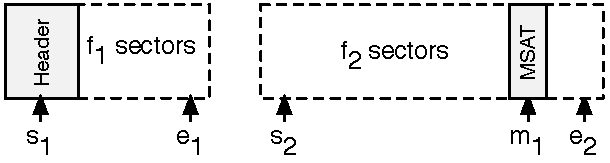
\includegraphics[width=\columnwidth]{carving/msatcarving}
\caption{In Bifragment Carving with Constant Size and Known Offset the
sectors $s_1$ and $m_1$ and $f_1+f_2$ are known; the carver must find
$e_1$, $s_2$ and $e_2$.}\label{msatcarving}
\end{figure}

Applying this carver to the 2006 Challenge we were able to recover all of the Microsoft Word
and Excel files that were split into two pieces. However, in one case
we had numerous false positives---files that would open in Microsoft Word but
which obviously contained incorrect data. The files opened in Word
because our MSOLE validator was able to produce file objects that
contained valid CDH, MSAT, SAT and SSAT, but which still had
substituted internal sectors. Some of the files opened instantly in
Word while others took many tens of seconds to open. However, the
number of file positives was low, and we were able to manually
eliminate the incorrect ones.

One of the Office files in the  challenge was in three pieces. Using
two of these fragments Our carver produced a file that could be opened
in Word and that contained most but not all of the text. Using this
text we were able to locate a source file on the Internet that was
similar but not identical to the file in the Carving
challenge. However, enough of the 512-byte sectors were the same that
we were able to determine the outlines of the three fragments. We then
manually carved these three fragments into a single file, opened it,
and verified that it was correct.


\section{Hash Based Carving}

\subsubsection{Hash-Based  Carving with frag\_find}\label{hash-based}
Carving is traditionally defined in computer forensics as the
searching for data objects based on \emph{content}, rather than
following pointers in metadata\cite{garfinkel:carving07}. Traditional
carvers operate by searching for headers and footers; some carvers
perform additional layers of object validation. Hash-based carving, in
contrast, searches a disk for ``master'' files already in a corpus by
performing sector-by-sector hash comparisons.

\newcommand{\master}{\textbf{master}\xspace}
%\newcommand{\image}{\textbf{image}\xspace}
\newcommand{\filemap}{\texttt{filemap}\xspace}
\newcommand{\shamap}{\texttt{shamap}\xspace}
We have developed a tool called |frag_find| that achieves high-speed
performance on standard hardware. Here we describe the algorithm using
the terminology proposed by Dandass
\etal~\cite{dandass2008,collange2009}, although our algorithm 
does not require their hardware-based acceleration techniques that
are the basis of their research:

\begin{compactenum}
\item For each \master file a \filemap data structure is created that
  can map each master file sector to a set of sectors in the image
  file. A separate \filemap is created for each master.
\item Every sector of each master file is scanned. For each sector the
  MD5 and SHA-1 hashes are computed. The
MD5 code is used to set a corresponding bit in a $2^{24}$ bit
Bloom filter. The SHA-1 codes are stored in a data structure called
the \shamap that maps SHA-1 codes to one or more sectors in which that
hash code is found. 
\item Each sector of the image file is scanned. For each sector
  the MD5 hash is computed and the corresponding bit checked in
  the Bloom filter. This operation can be done at nearly disk
  speed. Only when a sector's MD5 is found in the Bloom filter is
  the sector's SHA-1 calculated. The \shamap structure is consulted;
  for each matching sector found in the \shamap, the sector number of
  the IMAGE file is added to the corresponding
  sector in each master \filemap.
\item Each \filemap is scanned for the longest runs of
  consecutive image file sectors. This run is noted and then removed from
  the \filemap. The process is repeated until the \filemap contains no
  more image file sectors. 
\end{compactenum}

Our hash-based carving algorithm covers both fragmented master files and the
situation where portions of a master are present in multiple locations
in the image file.

Our original hash-based carving implementation used
Adler-32\cite{RFC1950} instead of MD5 as the fast hash, but subsequent
testing found that most MD5 implementations are actually faster than
most Adler-32 implementations due to extensive hand-optimization that
the MD5 implementations have received. Although the new algorithm
could dispense with SHA-1 altogether and solely use MD5, the MD5
algorithm is known to have deficiencies. If the results of hash-based
carving are to be presented in a court of law, it is preferable to use
SHA-1. To further speed calculation we found it useful to precompute
the SHA-1 of the NULL-filled sector; whenever the system is asked to
calculate the value of this sector, this value is used instead.

We prefer to use \emph{sectors} for hash-based
carving because they are the minimum allocation unit of the disk
drive. Larger block sizes are more efficient, but larger blocks
complicate the algorithm because of data alignment and partial write
issues. As a result, hash-based carving may fail to identify valid
data when used with block sizes larger than the sector size.


\section{Carving Challenges}

Carrier, Casey and Venema created the 2006 DFRWS Carving Challenge
to spur innovation in carving
algorithms~\cite{dfrws2006-challenge}. The Challenge consisted of a
49,999,872 byte ``challenge file'' containing data blocks from text
files, Microsoft office files, JPEG files, and ZIP 
archives, but having no file system metadata such as inodes or
directory entries. Some of the files in the Challenge were
contiguous, while others were split into two or three fragments. The
goal was to reconstruct the original files
that had been used to create the challenge. 




%\setcounter{chapter}{5}%\chapter{Unicode}
\label{chap:unicode}

Unicode is a continual source of frustration and problems for
developers and users of digital forensic tools. Designed in the 1990s
as a single code set capable of representing all of the world's
languages in the past, present and future, Unicode has largely
realized this goal. Today you can type languages with non-Roman
characters such as Russian or Japanese into a web browser or word
processor and generally produce acceptable looking documents. Most
application programs will even work with right-to-left languages like Arabic, 
Hebrew and Syriac, although support is somewhat inconsistent. Unicode
has also been a boon for graphic designers, who now have a dizzying
array of symbols with which they can work.

Unicode has been less kind to the world of digital forensics, for the
simple reason that Unicode makes it possible to have a wide variety of
byte representations within digital documents that display the same
way on a computer screen, print the same way on page, and are required
by the Unicode standard to be interpreted in the same manner.  As of
this document's writing in 2011, the majority of computer forensic
programs are simply not up to the challenge. 

As a result we see frequently characteristic failings when forensic
tools are presented with Unicode text:
\begin{itemize}
\item Unicode text frequently does not display properly, and it may
  not display at all.
\item Searches performed with forensic tools may not find names and
  keywords that are clearly 
  visible when a document is viewed with a native application.
\item \emph{Any other problems?}
\end{itemize}

One reason for the poor coverage of computer forensic tools may be
that most of today's tools are developed in the United States, and it
is possible to work broadly with computer systems in the US using
ASCII alone. Another issue may be that many computer forensic tools
are written in the C programming language, and the standard C string
type (\emph{char *}) cannot be used to represent Unicode that is in
the UTF-16 or UTF-32 encodings, as strings in these encodings invariably
contain NULL characters. Software developed outside the US tends to
have much better support for Unicode---perhaps for the simple reason
that currency symbols used by most countries of the world (\eg \pounds, \EURtm\xspace and \textyen)
cannot be represented using 7-bit codes, and thus programmers outside
the US are frequently forced to deal with these issues.

\begin{figure}
\begin{description}
\item[ASCII]
\item[code point]
\item[Baudot]
\item[EBCDIC]
\item[encoding]
\item[glpyh]
\item[grapheme]
\item[font]
\item[Shift JIS]
\item[Unicode]
\item[UTF-7]
\item[UTF-8]
\item[UTF-16]
\item[UTF-16BE]
\item[UTF-16LE]
\end{description}
\caption{Terminology}
\end{figure}

\section{Codes and Semantic Meaning}

The mechanization of writing has had a fundamental limitation from the
days of Gutenberg to the modern age. An unlimited number of
characters and designs can be created with pen and paper, but until
recently mechanical systems were limited to a relatively small number
of \emph{glpys} that could be represented. For example, in order to
print with movable type (as Gutenberg did), it is necessary to have a
piece of piece of \emph{type} for each glyph that is intended for the
printed page. 

\sgraphic{art/Metal_movable_type.jpg}{Movable metal type, and
  composing stick, descended from Gutenberg's press. Note: the plate says - ``The
  quick brown fox jumps over the lazy dog and feels as if he were in
  the seventh heaven of typography together with Hermann Zapf, the
  most famous artist of the''.  Photo by Willi Heidelbach; used with
  permission. See \texttt{http://en.wikipedia.org/wiki/File:Metal\_movable\_type.jpg}}

\emph{TK: Insert more information about the history of alphabetical
  order and the assignment of numbers to letters.}

\emph{TK: Insert information about Morse Code}

\subsection{Baudot and 5-Level Code for Teleprinters}

\emph{TK: Insert something about Baudot}

\subsection{ASCII}

\emph{TK: History of ASCII}

\subsection{Attempts to Internationalize ASCII}

\emph{TK: Brief history of font representation in Asia and why it
  matters for forensics.}

\subsection{Unicode}

\emph{TK: Brief history of Unicode through Unicode 5}

Unicode 1.0 (1991--1995) was a 16-bit code. Microsoft Windows still uses this version of Unicode for file names, and as a result certain Unicode characters cannot be used in filenames.

Starting with Unicode 2.0 (July, 1996) Unicode was expanded to cover the range U+0000..U+10FFFF. Each Unicode code point can be \emph{encoded} as a sequence of bytes. Somewhat confusingly, there are many different sequences of bytes that can be used to represent the same code point. Each of these encoding systems has advantages for different applications, so we have them all and Unicode-aware string libraries can easily convert from one encoding to another.

The most common Unicode encoding in the Western world is UTF-8, a
variable length code that  codes ASCII  as  byte values and other
scripts with sequences between two and four bytes.  UTF-16 codes code
points U+0000..U+FFFF as 16-bit values and other values with four bytes. UTF-32 codes all Unicode characters as four bytes, which is the least efficient space wise but which is easiest to work with inside a computer system. UTF-16 and UTF-32 both come in Big Endian and Little Endian varieties. (UTF standards for \emph{Unicode transforamtion format}.)

Unicode has 66 invalid code points, including U+FFFE and U+FFFF.

Remember that Unicode is used to encode \emph{scripts}, not languages. Scripts are used for displaying languages in written form. This is an important distinction, because the LATIN CAPITAL LETTER A (``A'', or U+0041) () is a A no matter whether the language is English or French. On the other hand, the GREEK CAPITAL LETTER ALPHA (``
\includegraphics{uni/unicode_alpha}'', or U+0391) looks like an A, but it isn't. This is done so that sort order will be preserved within alphabets, and to preserve round-tripping between Unicode and other coding formats.

\section{Unicode Today: Design and the Forensic Challenge}

When working with Unicode in a forensic context, the most important
thing to remember is that Unicode is fundamentally based on \emph{code
points} and not on the specific \emph{encoded characters} that we may
encounter when performing forensic analysis.

A Unicode code point is an
idealized character that has a value. The first 127 of these map to
ASCII (the American Standard Code for Information Interchange). You
may be aware that capital A is a 65 (or 0x41). In Unicode most
characters are between 0 and 65535; they are written as a U+ followed
by a 4-character hex code, so the capital A is U+0041. Each Unicode
code point has a name as well, which is traditionally typed using
CAPITAL LETTERS.

The Unicode Character Database defines all of the Unicode code points. Different ranges of code points are used for different purposes. The first 10 ranges are shown in \tabref{unicode-ranges}
\begin{table}
\begin{Verbatim}
0000..007F; Basic Latin
0080..00FF; Latin-1 Supplement
0100..017F; Latin Extended-A
0180..024F; Latin Extended-B
0250..02AF; IPA Extensions
02B0..02FF; Spacing Modifier Letters
0300..036F; Combining Diacritical Marks
0370..03FF; Greek and Coptic
0400..04FF; Cyrillic
0500..052F; Cyrillic Supplement
0530..058F; Armenian
0590..05FF; Hebrew
0600..06FF; Arabic
0700..074F; Syriac
0750..077F; Arabic Supplement
0780..07BF; Thaana
07C0..07FF; NKo
\end{Verbatim}
\caption{Unicode code point blocks for Unicode code points between \texttt{U+0000} and \texttt{U+07FF}. The entire file can be found at \texttt{http://unicode.org/Public/UNIDATA/Blocks.txt}}\label{unicode-ranges}
\end{table}

Note that while Unicode code points are frequently referred to as Unicode
``characters,'' this isn't strictly true, as code points can represent
information other than printable glyphs. Unicode has all of ASCII's
non-printing ``characters,'' including SPACE (U+0020) and LINE
FEED (U+000A) and BELL (U+0007). Unicode also has a spaces associated
with typesetting, including EM SPACE (U+2003), UN SPACE (U+2002), and
even THIN SPACE (U+2009). But Unicode also has special codes such as 
LEFT-TO-RIGHT MARK (U+200E) and RIGHT-TO-LEFT MARK (U+200F) that
control the direction that the glyphs are laid on the page. 

Unicode code points can be encoded in multiple variants. UTF-8 is the
most common in the US. UTF-8 encodes all ASCII characters as
themselves, and codes the rest as a variable length code between 2 and
6 characters long. This doesn't work so well for Chinese, most of
which take 3 bytes in UTF-8.  So in China and other Asian countries,
you'll find a lot of UTF-16, which codes most Unicode characters as
2-bytes. If the big byte comes first it is UTF-16BE (``Big Endian''),
with the capital A encoded as 0x00 0x41. If the little byte comes
first the coding is UTF-16LE (``Little Endian''), with the capital A
encoded as 0x41 0x00. There is also an encoding called UTF-7, in which
every character is coded within the ASCII character set. Avoid it.

Ideally every block of  Unicode-encoded data is preceeded with the Byte Order
Mark, the Unicode ZERO WIDTH NO-BREAK
SPACE (U+FEFF). This code point, stored at the beginning Unicode
block, allows the reader to infer if the data is stored as UTF-8, UTF-16LE, UTF-16BE, UTF-32LE or
UTF-32BE. Byte order detection relies on the fact that U+FFFE is an
invalid Unicode character. If the beginning of  file contains the
hex characters |FE FF| then the file is UTF-16BE because the big
character is first. \tabref{table-bom} shows various codings of the
Unicode byte order mark.

Unfortunately, many (perhaps most) sequences of Unicode-encoded bytes
do not being with the BOM. Instead, coding is provided by a higher
level protocol. For example, many HTML pages begin with the following
four lines to indicate that the web page is stored as UTF-8:

\begin{Verbatim}
<!DOCTYPE html>
<html xmlns="http://www.w3.org/1999/xhtml" xml:lang="en-US" lang="en-US">
<head>
   <meta http-equiv="content-type" content="text/html; charset=utf-8" />
\end{Verbatim}

The observant reader will note that decoding the HTML page to
determine the page's encoding requires knowing the page's
encoding, which is not possible. In practice web browsers attempt to
infer the pages encoding by trying multiple decodings of the first few
bytes of the file until they discover the |<!DOCTYPE| or |<html| tag.


\begin{table}
\begin{tabular}{cl}
Unicode Encoding & Hex character sequence\\
\hline
UTF-8 & |EF BB BF|\\
UTF-16BE & |FE FF|\\
UTF-16LE & |FF FE|\\
UTF-32BE & |00 00 FE FF|\\
UTF-32LE & |FF FE 00 00|\\
\end{tabular}
\caption{Encodings and representations of Unicode ZERO WIDTH NO-BREAK
SPACE (U+FEFF), the Unicode byte order Mark.}\label{table-bom}
\end{table}


\subsection{Unicode Goals}

\emph{TK: Insert Unicode Goals}

\subsection{Unicode 6.0}

\section{Unicode and Forensic Software}

Unicode poses a variety of challenges for authors of forensic
software:

\begin{enumerate}
\item Although many Unicode strings can be freely inter-converted to
  ASCII, the vast majority cannot. This means that code written and
  tested in the United States frequently fails when presented with
  real-world Unicode strings from other countries.
\item File names may contain Unicode characters, and those Unicode
  characters are typically stored differently on Windows, MacOS and
  Unix. 
\item For programs running natively on an operating system, different
  APIs may return the same file names with different Unicode
  encodings.
\item Original byte sequences from subject media needs to be
  preserved inside a forensic program. However data structures 
  that are \emph{required} to contain valid Unicode nevertheless may
  actually contain invalid encodings. This means that forensic
  software must be able to handle invalid Unicode data in a sensible manner.

\end{enumerate}

In practice different programmers have resolved the Unicode problem in
different ways. The result is that different forensic tools perform
differently when faced with the same evidence.

\subsection{Unicode Normalization}

Consider the case of the \~n, a letter that is commonly used (and
misused) in Spanish. There are two different ways to represent this in
Unicode: with the Unicode character |U+00F1| (LATIN SMALL LETTER N
WITH TIDLE), and with two character sequence U+006E (LATIN SMALL
LETTER N) followed by |U+0303| (COMBINING TILDE). Not only do these
characters display the same way (as a \~n), \emph{they both describe
  the same  characters}.

The Unicode standard defines two kinds of sameness: \emph{canonical
equivalence} and \emph{compatibility equivalence}.

\begin{description}
\item[Canonical equivalence] results from
the application of one or more combining characters and is considered
a strong equivalence: the abstract character is the same no matter
whether it is represented by a single Unicode code point or by
multiple code points with the aid of combining characters. Likewise
the order in which combining characters are used does not
matter. Combined characters always display the same way as base
characters with combiners. the use of combining characters results in
the same abstract character as the uncombined form. 

% ⑨
% ❾
% 
\PreloadUnicodePage{36}
\item[Compatibility equivalence] is used to denote sequences that have the same semantic
meaning but may appear visually distinct. For example, TR15 says that a
SUPERSCRIPT NINE (⁹) (U+2079) and a SUBSCRIPT NINE (₉) (U+2089) are
compatibility equivalent characters, because they are both a
nine. This is confusing for people who are used to doing superscripts
and subscripts in Microsoft Word or LaTeX; both of those systems do
superscripts and subscripts by shrinking the font and changing the
baseline. The unicode also has CIRCLED DIGIT NINE (U+2468) 
\includegraphics{uni/unicode_2468} and
DINGBAT NEGATIVE CIRCLED DIGIT NINE 
\includegraphics{uni/unicode_277E} (U+277E). This means that the
number 
\includegraphics{uni/unicode_2468}
\includegraphics{uni/unicode_2468} and 99 have the same sort order, even though they have
wildly different Unicode characters
 
Another example is HEBREW LETTER ALEF (
\includegraphics{uni/unicode_05D0}) (U+05D0) and ALEF SYMBOL (
\includegraphics{uni/unicode_2135}))
(U+2135). Wow, those two look really similar. But if you
copy-and-paste the first one into a document you'll see that it's in
right-to-left mode while the second one is in left-to-right
mode. That's because the first one is for hebrew and the second is for
math. There is also HEBREW LETTER WIDE ALEF 
\includegraphics{uni/unicode_FB21} (U+FB21) which is
probably for use with Japanese (they like having double-wide
characters because it matches the Kanji, and you'll note that this
Unicode's value is up in the FBxx range.


\end{description}

To compare Unicode strings it is necessary to put them into a standard
form, a process called \emph{noramlization} (\figref{unicode-normalization}). In normalization,
sequences of Unicode code points that are part of the same equivalence classes are transformed
so that they have the identical code points. The strings can then be
compared (either directly, code-point-by-code-point, or by
transforming the strings yet again into a Unicode encoding such as
UTF-8 or UTF-32LE). 

\begin{figure}[t]

The Unicode Standard actually defines two kinds of equivalences
between characters: \emph{canonical equivalence} and
\emph{compatibility equivalence.} Canonical equivalence results from
the application of one or more combining characters and is considered
a strong equivalence: the abstract character is the same no matter
whether it is represented by a single Unicode code point or by
multiple code points with the aid of combining characters. Likewise
the order in which combining characters are used does not
matter. Combined characters always display the same way as base
characters with combiners. the use of combining characters results in
the same abstract character as the uncombined form. Compatibility
Equivalence is used to denote sequences that have the same semantic
meaning but may appear visually distinct.) \\
~\\
The Unicode Normalization process is described in  Unicode Technical Annex \#15: Unicode Normalization \url{http://unicode.org/reports/tr15/}. There are  four different normalization forms:\\
\\
\begin{centering}
\begin{tabular}{|l|l|}
\hline
Title & Description\\
\hline
Normalization Form D (NFD)	& Canonical Decomposition\\
\hline
Normalization Form C (NFC)	& Canonical Decomposition,\\
                            & followed by Canonical Composition\\
\hline
Normalization Form KD (NFKD) & Compatibility Decomposition\\
\hline
Normalization Form KC (NFKC) & Compatibility Decomposition,\\
                             &followed by Canonical Composition\\
\hline
\end{tabular}
\end{centering}
\\
The Unicode standard uses the word \emph{singleton} to refer to a character that has a decomposition of a single unicode character.
\\
The NFD form decomposes a combined character into the base character and the combiner, whereas the NFC form does the reverse. As a result, NFD forms result in larger byte representations than NFC forms. The NFKD and NFKC forms add a compatibility decomposition---for example, decomposing the ``fi'' ligature into the characters ``f'' and ``i'' and transforming superscript and subscript numbers to unscripted letters. Among other things, this transformation improves the chances of string searches resolving correctly.
\\
Please refer to UAX \#15 for full details.
\caption{Unicode equivalence and normalization Forms, from UAX\#15}\label{unicode-normalization}
\end{figure}

Unicode  has four different normalized forms. Once normalized, the strings can be directly compared in the Unicode domain (if you have a Unicode string object that can do so).
Alternatively, the strings can then be encoded into a byte-level representation such as UTF-8 and compared byte-for-byte. 

\tabref{unicode-n} shows the legacy approaches for representing the character and the many byte sequences that can be used to represent this character in Unicode. 

\begin{table}
\begin{tabular}{llll}
\hline
Encoding & Hex    & Notes & \\
\hline
Microsoft Windows &  |F1|      &  Type with ALT 241\\
Mac Roman         &  |96|      & Option-n n \\
Linux             &            & Ctrl+Shift u00F1\\
\hline\\
\multicolumn{4}{l}{\emph{Unicode ``n'' with the ``\~{}'' Combining Character:}}\\
UTF-8     & |6E CC 83|\\
UTF-16 BE & |00 6E 03 03|\\
UTF-16 LE & |00 6E 03 03|\\
UTF-32 BE & |00 00 00 6E 00 00 03 03|\\
UTF-32 LE & |6E 00 00 00 03 03 00 00|\\
\hline
\\
\multicolumn{4}{l}{\emph{Normalized Unicode ``\~n'':}}\\
UTF-8   &  |C3 B1|          & \\
UTF-16 BE         &  |00 F1|          & \\
UTF-16 LE         &  |F1 00|          & \\
UTF-32 BE         &  |00 00 00 F1|    & \\
UTF-32 LE         &  |F1 00 00 00|    & \\
\hline
\end{tabular}
\caption{A variety of ways to represent the character "\~n" (LATIN SMALL LETTER N WITH TILDE) in Unicode, and a small Python program that will create a file containing the character.}\label{unicode-n}
\end{table}

\subsection{Unicode and Python}

The Python programming language  support for Unicode and most program written in Python will more-or-less work with Unicode data without significant work on the part of the programmer. This does not mean that you can ignore Unicode issues, however. If you write programs that work with user-supplied data (as all forensic programs do), then you must be sure that your program operates properly with Unicode no matter what format it is provided. Python makes this somewhat easier with built-in functions for transforming Unicode strings into encoded representation and the |unicodedata| class that has a large database of Unicode information.

Unfortunately, support for Unicode changed significantly between Python 2 and Python 3. Because both versions of Python are widely in use, this section will provide a small introduction to each.

\subsubsection{Unicode and Python 2}
Python 2 has support for two kinds of strings. The |string| data type is for traditional strings of single-byte characters (ASCII or Windows-1252), for which the number of characters in the string is precisely equal to the number of bytes. Python 2 also has a |unicode| data type which is an array of |unichar| characters. Unicode strings are specified by placing a lower-case |u| before the quotation mark that starts the string.

Python 2 assumes that your program will be written in ASCII, but you can change this default by specifying a coding on the first or second line of your program. If you open a file with |open()| and read the bytes the result will be type |str|.

Below is a small program that was used to create the data in \tabref{unicode-n}:

\begin{Verbatim}
# -*- coding: utf-8 -*-
#

import unicodedata,sys

encodings=['mac roman','latin1','utf-8','utf-16 le','utf-16 be',
           'utf-32 le','utf-32 be']
nn     = unicodedata.normalize("NFC",u"ñ")
print type(nn),unicodedata.name(nn)
for encoding in encodings:
  print "%9s: " % format(encoding),
  for ch in nn.encode(encoding):
      print "%02x " % ord(ch),
  print
\end{Verbatim}

Notice that there's a small slight-of-hand going on with this
program. In the actual program code the ``ñ'' is stored as the hex
sequence |C3 B1|. However when Python reads this sequence the parser
automatically decodes the UTF-8 into the Unicode code point U+00F1,
which is then put into the string. 

Alternatively, the variable \texttt{nn} could be set with an escaped
Unicode sequence. Normalization is not required because the value is
provided in a normalized form:

\begin{Verbatim}
nn   = u"\u00F1"
\end{Verbatim}

If the character was entered in the source code as a two-byte vector,
it would be necessary to join it into a string and then to decode that
string as UTF-16 before normalization:

\begin{Verbatim}
buf  = ['\x00','\xF1']
nn   = unicode.normalize("NFC",("".join(buf)).decode('utf-16 be'))
\end{Verbatim}

\emph{NOTE: THIS WOULD MAKE MORE SENSE IF WE START THE EXAMPLE BY
  PRESENTING WITH THE ESCAPED UNICODE SEQUENCE AND THEN SHOW HOW TO
  EMBED THE CHARACTER IN THE DOCUMENT.}


And here is the output:

\begin{Verbatim}
$ ./unicode_demo2.py 
<type 'unicode'> LATIN SMALL LETTER N WITH TILDE
mac roman:  96 
   latin1:  f1 
    utf-8:  c3  b1 
utf-16 le:  f1  00 
utf-16 be:  00  f1 
utf-32 le:  f1  00  00  00 
utf-32 be:  00  00  00  f1 
$ 
\end{Verbatim}

If you don't want to put hard-coded UTF-8 characters in your source code file (some editors may complain), the string |u"ñ"| can also be written |u"\u00f1"|. Characters outside the BMP are encoded with 8-digits and a capital U, so the U+1D11E (MUSICAL SYMBOL G CLEF), is entered as |u"\U0001D11E"|.

One last thing---most version of Python use UTF-16 internally, meaning that the Supplementary Planes are accessed with Surrogate Pairs. This can cause some weirdness, because a single code point is actually represented by two UTF-16 characters:

\font\musixfont="musix11" at 7pt
\newcommand\cleff{{\musixfont G}} % G-Cleff symbol from MusixTeX fonts
\begin{Verbatim}[commandchars=\$\{\}]
>>> cleff=u"\U0001D11E"
>>> len(cleff)
2
>>> type(cleff)
<type 'unicode'>
>>> cleff[0]
u'\ud834'
>>> cleff[1]
u'\udd1e'
>>> import sys
>>> sys.stdout.write(cleff.encode('utf-8')+"\n")
$cleff
>>> 
\end{Verbatim}
%$
This problem of surrogates is present in both Python 2 and Python 3
(as well as in the native Windows API). Python can be compiled to use UCS-4
internally, but that isn't done. Allegedly the reason is performance
reasons---UCS-4 strings take up twice the size of UTF-16 strings---but
the total overhead required by 4-byte characters may be minimal. 


\subsubsection{Unicode in Python 3}
In Python 3 all strings are  Unicode strings, and the Unicode type has been abolished.  If you open and read the contents of a file the resulting data type will depend on how the mode and codec provided when the file is opened.

For example, consider a simple file on the Unix system that contains the ASCII string "Hello World!" and a newline:

\begin{Verbatim}
$ echo 'Hello World!' > hello.txt
$ cat hello.txt
Hello World!
$ ls -l hello.txt
-rw-r--r--  1 simsong  staff  13 Oct 23 16:09 hello.txt
$ 
\end{Verbatim}

Opening and reading the content of this file in text mode will yield a Unicode string:
\begin{Verbatim}
>>> open("hello.txt","r").read()
'Hello World!\n'
>>> type(open("hello.txt","r").read())
<class 'str'>
>>> 
\end{Verbatim}

If you want a binary string, you must open the file in binary mode:

\begin{Verbatim}
>>> open("hello.txt","rb").read()
b'Hello World!\n'
>>> type(open("hello.txt","rb").read())
<class 'bytes'>
>>> 
\end{Verbatim}

Notice that there is a |b| at the beginning of the string, indicating that it is a byte string, and not a Unicode string.

The distinction between bytes and Unicode text is important when you are trying to read data from files that is not valid Unicode. Consider a file that is filled with the 16 hex FF characters:

\begin{Verbatim}
$ ls -l file.txt 
-rw-r--r--  1 simsong  staff  16 Oct 23 16:15 file.txt
$ xxd file.txt 
0000000: ffff ffff ffff ffff ffff ffff ffff ffff  ................
$ 
\end{Verbatim}
%$
The issue here is that the sequence |FF FF FF FF| is not valid Unicode
in \emph{any} Unicode encoding (there is no U+FFFF). Python 3 defaults
to text mode, which means it expects all text files that are read to contain valid Unicode. Therefore, if we try to read this file with a legacy Python 2 program using Python 3, we'll get a puzzling error:

\begin{Verbatim}
>>> f = open("file.txt","r")
>>> f.read()
Traceback (most recent call last):
  File "<stdin>", line 1, in <module>
  File "/opt/local/Library/Frameworks/Python.framework/Versions/3.2/lib/python3.2/codecs.py", line 300, in decode
    (result, consumed) = self._buffer_decode(data, self.errors, final)
UnicodeDecodeError: 'utf8' codec can't decode byte 0xff in position 0: invalid start byte
>>> 
\end{Verbatim}

The solution is to open the file in binary mode:

\begin{Verbatim}
>>> f = open("file.txt","rb")
>>> f.read()
b'\xff\xff\xff\xff\xff\xff\xff\xff\xff\xff\xff\xff\xff\xff\xff\xff'
>>> 
\end{Verbatim}

And here is a rewrite of the Unicode-aware program we showed in the previous section:
\begin{Verbatim}
#!/usr/bin/env python3.2 
# -*- coding: utf-8 -*- 
# 

import unicodedata
encodings=['latin1','utf-8','utf-16 le','utf-16 be',
           'utf-32 le','utf-32 be']
nn     = unicodedata.normalize("NFC","ñ")
print(type(nn),unicodedata.name(nn))
for encoding in encodings:
  print("{:9}: ".format(encoding),end="")
  for ch in nn.encode(encoding):
      print("{:02x} ".format(ch),end="")
  print()
\end{Verbatim}

Python 3 also lets you write the string string |"ñ"| as|"\u00f1"|. Note that you do not need to prefix the string with a |u| (in fact, you can't) because all Python 3 strings are unicode.


\subsubsection{The Python \texttt{unicodedata} module}
You should become familiar with the Python |unicodedata| module. This module, present in both Python 2 and 3, provides a number of functions including:

\begin{itemize}
\item |lookup()| and |name()|, to look up a Unicode character by name and return the name of a unicode character.
\item |category()|, to return the category to which a Unicode character is defined.
\item |normalize()|, an implementation of the Unicode normalization algorithm.
\end{itemize}

\subsubsection{Missing from Python's Unicode Support}
Christopher Lenz notes that Python's Unicode implementation is actually quite poor and contains only the minimum needed.\url{http://www.cmlenz.net/archives/2008/07/the-truth-about-unicode-in-python} In particular, he notes, there is no support in Python 2 or 3 for:

\begin{itemize}
\item Collation
\item Special case conversion
\item Regular expressions
\item Text segmentation
\item bidirectional text handling
\end{itemize}

What this means in practice is that Python 3 thinks that the string |'café'| sorts lexicographically after |'caff'| because |é| (U+00E9, LATIN SMALL LETTER E WITH ACUTE) has a higher character code than |f| (U+0066, LATIN SMALL LETTER F). 

He's right, but it's not clear that this is going to be fixed anytime soon.

\subsection{Unicode and C/C++}
There are two primary ways of representing Unicode strings in C/C++ programs:
\begin{enumerate}
\item The string can be encoded in UTF-8 and stored in a |char *| buffer or a or C++ |std::string|. This approach takes advantage of the fact that UTF-8 encoding never codes NULLs.
\item The string can be stored ``natively'' in with ``wide characters,'' the C/C++ |wchar_t| type and the C++ |std::wstring|.   Windows XP uses a short to hold a |wchar_t|, while Linux and MacOS use a 4-byte value and store UTF-32 characters.  
\end{enumerate}

Windows handles Unicode characters outside the BMP through the use of Surrogate characters. Surrogates are essentially combinations of two UTF-16 characters to stand for a single Unicode character that has a value over U+FFFF. Windows Vista has three macros for working with surrogate pairs, |IS_HIGH_SURROGATE|, |IS_LOW_SURROGATE|, and |IS_SURROGATE_PAIR|. Support for surrogate pairs is spotty throughout the Windows ecology. More information can be found at \url{http://msdn.microsoft.com/en-us/library/windows/desktop/dd374069%28v=vs.85%29.aspx}.

Conversions between various encodings can be done with GNU libiconv (\url{http://www.gnu.org/s/libiconv/}). If you are using C++ you may wish to use the UTF8-CPP module (\url{http://utfcpp.sourceforge.net/}).





\subsection{Unicode and Java}
Java officially uses Unicode as its character and string encoding. Unfortunately the Java standard did not adopt Unicode code points as an abstract representation---it adopted a 16-bit representation for characters. That's because Java was standardized in the day of Unicode 1.0, when Unicode was a 16-bit code.

\emph{How does Java handle things outside of the BMP?}


\subsection{\be and Unicode: a case history}
One tool that has been modified to understand Unicode is
\be, the author's bulk data analysis tool. Making
this tool Unicode-aware has been a time consuming and error-prone
task, and it is not finished yet. One of the primary functions of \be
is to find and report all URLs that appear in a disk image under
analysis. Unicode impacts this task in at least four ways:

\begin{enumerate}
\item URLs may be encoded as ASCII, UTF-8 or UTF-16 in the disk image
  under analysis. Thus it is necessary for \be to recognize a URL in
  any of these variant encodings.\label{url-encoding}
\item \be produces a histogram that reports the number of times each
  URL appears in the disk image. Thus, it is necessary to recognize
  that URLs present in different encodings represent the same URL.\label{url-matching}
\item The URL's \emph{path} may contain unicode characters.\label{url-path}
\item The URL's \emph{domain name} may contain an internationalized
  host name.\label{url-domain}
\end{enumerate}

Currently \be handles the first two of these problems.

\subsubsection{Evolution of Unicode Handling in \be}
When it was first released in 2010, \be had a simplistic handling of
Unicode URLs: the program simply looked for text strings in which
every-other character was an ASCII NULL and removed the
NULLs. Non-ASCII characters in output were changed to the underbar
character. This approach handled case \ref{url-encoding} and case
\ref{url-matching} above, but it caused a problem for users: the data
reported by \be did not actually exist. (See
\figref{url_histogram-0.7.16} for an example of the output from \be's
  \emph{url\_histogram.txt} and \emph{url.txt} files.)

As the result of user complaints, Version 1.0 of \be was modified to
report the actual text extracted from the disk image, even for cases
in which the text was UTF-16. Now the information in the \be report
was an accurate representation of what was in the disk
image. Although this output worked well with automated processing, it
made  manual review of the file considerably harder (\figref{url_histogram-1.0.2}).

For version 1.1 of \be the histogram generation routine was modified
to detect the presence of UTF-16LE and UTF-16BE in the feature
files. These strings are transformed to UTF-8 before the histogram
bins are calculated. The revised histogram program also tracks how
many of the source strings were transformed and reports this in the
histogram output as well (\figref{url_histogram-1.1.0}). The result is
tool output that is correct, usable for automated processing, and
usable for manual analysis.


\begin{figure}
\begin{Verbatim}[fontsize=\footnotesize]
n=8164  http://components.groove.net/Groove/Components/Root.osd?Package=net.groove.Groove.Tool
  Components.GrooveCommonComponents_DLL&Version=0
n=6257  http://www.microsoft.com/contentredirect.asp.
n=3031  http://ocsp.verisign.com0

11548143368     http://components.groove.net/Groove/Components/Root.osd?Package=net.groove.Gro
  ove.ToolComponents.GrooveCommonComponents_DLL&Version=0       ___URL(_http://components.groo
  ve.net/Groove/Components/Root.osd?Package=net.groove.Groove.ToolComponents.GrooveCommonCompo
  nents_DLL&Version=0&Factory
11548144224     http://components.groove.net/Groove/Components/Root.osd?Package=net.groove.Gro
  ove.ToolComponents.GrooveCommonComponents_DLL&Version=0       ___URL(_http://components.groo
  ve.net/Groove/Components/Root.osd?Package=net.groove.Groove.ToolComponents.GrooveCommonCompo
  nents_DLL&Version=0&Factory
11548145356      http://components.groove.net/Groove/Components/Root.osd?Package=net.groove.Gr
  oove.ToolComponents.GrooveCommonComponents_DLL&Version=0      ___URL6_http://components.groo
  ve.net/Groove/Components/Root.osd?Package=net.groove.Groove.ToolComponents.GrooveCommonCompo
  nents_DLL&Version=0&Factory
\end{Verbatim}
\caption{The first three lines of the \texttt{url\_histogram.txt}
  output file from \be version 0.7.16 processing the
  nps-2009-domexusers disk image, followed by three lines taken from
  the \texttt{url.txt} file of where the groove.net URL was
  found. Long lines have been wrapped; the continuation line begins
  with two spaces}\label{url_histogram-0.7.16}
\end{figure}

\begin{figure}
\begin{Verbatim}[fontsize=\footnotesize]
n=8164  h\000t\000t\000p\000:\000/\000/\000c\000o\000m\000p\000o\000n\000e\000n\000t\000s\000.
  \000g\000r\000o\000o\000v\000e\000.\000n\000e\000t\000/\000G\000r\000o\000o\000v\000e\000/\0
  00C\000o\000m\000p\000o\000n\000e\000n\000t\000s\000/\000R\000o\000o\000t\000.\000o\000s\000
  d\000?\000P\000a\000c\000k\000a\000g\000e\000=\000n\000e\000t\000.\000g\000r\000o\000o\000v\
  000e\000.\000G\000r\000o\000o\000v\000e\000.\000T\000o\000o\000l\000C\000o\000m\000p\000o\00
  0n\000e\000n\000t\000s\000.\000G\000r\000o\000o\000v\000e\000C\000o\000m\000m\000o\000n\000C
  \000o\000m\000p\000o\000n\000e\000n\000t\000s\000_\000D\000L\000L\000&\000V\000e\000r\000s\0
  00i\000o\000n\000=\0000\000
n=6257  h\000t\000t\000p\000:\000/\000/\000w\000w\000w\000.\000m\000i\000c\000r\000o\000s\000o
  \000f\000t\000.\000c\000o\000m\000/\000c\000o\000n\000t\000e\000n\000t\000r\000e\000d\000i\0
  00r\000e\000c\000t\000.\000a\000s\000p\000.\000
n=3031  http://ocsp.verisign.com0


11548143368     h\000t\000t\000p\000:\000/\000/\000c\000o\000m\000p\000o\000n\000e\000n\000t\0
  00s\000.\000g\000r\000o\000o\000v\000e\000.\000n\000e\000t\000/\000G\000r\000o\000o\000v\000
  e\000/\000C\000o\000m\000p\000o\000n\000e\000n\000t\000s\000/\000R\000o\000o\000t\000.\000o\
  000s\000d\000?\000P\000a\000c\000k\000a\000g\000e\000=\000n\000e\000t\000.\000g\000r\000o\00
  0o\000v\000e\000.\000G\000r\000o\000o\000v\000e\000.\000T\000o\000o\000l\000C\000o\000m\000p
  \000o\000n\000e\000n\000t\000s\000.\000G\000r\000o\000o\000v\000e\000C\000o\000m\000m\000o\0
  00n\000C\000o\000m\000p\000o\000n\000e\000n\000t\000s\000_\000D\000L\000L\000&\000V\000e\000
  r\000s\000i\000o\000n\000=\0000\000       \000\001\000\000\000\003\000\000\200URL(\001\000\0
  00h\000t\000t\000p\000:\000/\000/\000c\000o\000m\000p\000o\000n\000e\000n\000t\000s\000.\000
  g\000r\000o\000o\000v\000e\000.\000n\000e\000t\000/\000G\000r\000o\000o\000v\000e\000/\000C\
  000o\000m\000p\000o\000n\000e\000n\000t\000s\000/\000R\000o\000o\000t\000.\000o\000s\000d\00
  0?\000P\000a\000c\000k\000a\000g\000e\000=\000n\000e\000t\000.\000g\000r\000o\000o\000v\000e
  \000.\000G\000r\000o\000o\000v\000e\000.\000T\000o\000o\000l\000C\000o\000m\000p\000o\000n\0
  00e\000n\000t\000s\000.\000G\000r\000o\000o\000v\000e\000C\000o\000m\000m\000o\000n\000C\000
  o\000m\000p\000o\000n\000e\000n\000t\000s\000_\000D\000L\000L\000&\000V\000e\000r\000s\000i\
  000o\000n\000=\0000\000&\000F\000a\000c\000t\000o\000r\000y\000
\end{Verbatim}
\caption{The first three lines of the \texttt{url\_histogram.txt}
  output file from \be version 1.0.2 processing the
  nps-2009-domexusers disk image, followed by three lines taken from
  the \texttt{url.txt} file of where the groove.net URL was
  found. Long lines have been wrapped and indented with two spaces.}\label{url_histogram-1.0.2}
\end{figure}

\begin{figure}
\begin{Verbatim}
n=8164	http://components.groove.net/Groove/Components/Root.osd?Package=net.groove.Groove.Tool
  Components.GrooveCommonComponents_DLL&Version=0	(utf16=8164)
n=6257	http://www.microsoft.com/contentredirect.asp.	(utf16=6257)
n=3279	http://ocsp.verisign.com
\end{Verbatim}
\caption{The first three lines of the \texttt{url\_histogram.txt}
  output file and the first line of the \texttt{url.txt} files created
  by processing the
  nps-2009-domexusers disk image with \be version 1.1.0. The output from the \texttt{url.txt}
file is not included, as it is the same as in \figref{url_histogram-1.0.2}}\label{url_histogram-1.1.0}
\end{figure}

\section{Forensic Research in Unicode}

One way to understand UNICODE is to read the Unicode standard. Much of
it is available online, including the Code Charts. You can find it at:
http://www.unicode.org/versions/Unicode6.0.0/

``Unicode: A Universal Character Code,'' Digital Technical Journal,
Vol. 5, No. 3, Summer 1993. It's attached to this message.

Markus Kuhn, a computer security expert at Cambridge has put together
a UTF-8 and Unicode FAQ for Unix/Lunux. I highly recommend it, but you
may feel like you are coming into the middle of a discussion.
http://www.cl.cam.ac.uk/~mgk25/unicode.html



\section{Technical References to Review}
\begin{itemize}
\item Unicode Standard Annex \#15 --- Unicode Normalization Forms (\url{http://unicode.org/reports/tr15/})
\item Unicode Technical Report \#17 --- Unicode Character Encoding Model (\url{http://www.unicode.org/reports/tr17/}), discusses terms and encodings used in the Unicode standard.
\item Unicode Technical Report \#25 - Unicode Support for Mathematics \url{http://www.unicode.org/reports/tr25/}
\item Unicode Technical Report \#36 - Unicode Security Considerations \url{http://unicode.org/reports/tr36/}

\end{itemize}



% LocalWords:  encodings
        % October 27
\chapter{Hashing, Fuzzy Hashing, and Similarity Digests}

\section{Similarity Metrics}
\subsection{Binary Similarity}
\cite{dfrws2011:VassilRoussev}
\subsection{Text Similarity}
\cite{dfrws2011:ClayShieldsAndOphirFriederAndMarkMaloof}


1. “Security aspects of piecewise hashing in computer forensics,”
H. Baier and F. Breitinger, 6th International Conference on IT
Security Incident Management \& IT Forensics, May 2011. 
\verb+https://www.fbi.h-da.de/fileadmin/gruppen/FG-IT-Sicherheit/Publikationen/2011/2011_05_Baier_IMF2011.pdf+


%\setcounter{chapter}{5}\chapter{Unicode}
\label{chap:unicode}

Unicode is a continual source of frustration and problems for
developers and users of digital forensic tools. Designed in the 1990s
as a single code set capable of representing all of the world's
languages in the past, present and future, Unicode has largely
realized this goal. Today you can type languages with non-Roman
characters such as Russian or Japanese into a web browser or word
processor and generally produce acceptable looking documents. Most
application programs will even work with right-to-left languages like Arabic, 
Hebrew and Syriac, although support is somewhat inconsistent. Unicode
has also been a boon for graphic designers, who now have a dizzying
array of symbols with which they can work.

Unicode has been less kind to the world of digital forensics, for the
simple reason that Unicode makes it possible to have a wide variety of
byte representations within digital documents that display the same
way on a computer screen, print the same way on page, and are required
by the Unicode standard to be interpreted in the same manner.  As of
this document's writing in 2011, the majority of computer forensic
programs are simply not up to the challenge. 

As a result we see frequently characteristic failings when forensic
tools are presented with Unicode text:
\begin{itemize}
\item Unicode text frequently does not display properly, and it may
  not display at all.
\item Searches performed with forensic tools may not find names and
  keywords that are clearly 
  visible when a document is viewed with a native application.
\item \emph{Any other problems?}
\end{itemize}

One reason for the poor coverage of computer forensic tools may be
that most of today's tools are developed in the United States, and it
is possible to work broadly with computer systems in the US using
ASCII alone. Another issue may be that many computer forensic tools
are written in the C programming language, and the standard C string
type (\emph{char *}) cannot be used to represent Unicode that is in
the UTF-16 or UTF-32 encodings, as strings in these encodings invariably
contain NULL characters. Software developed outside the US tends to
have much better support for Unicode---perhaps for the simple reason
that currency symbols used by most countries of the world (\eg \pounds, \EURtm\xspace and \textyen)
cannot be represented using 7-bit codes, and thus programmers outside
the US are frequently forced to deal with these issues.

\begin{figure}
\begin{description}
\item[ASCII]
\item[code point]
\item[Baudot]
\item[EBCDIC]
\item[encoding]
\item[glpyh]
\item[grapheme]
\item[font]
\item[Shift JIS]
\item[Unicode]
\item[UTF-7]
\item[UTF-8]
\item[UTF-16]
\item[UTF-16BE]
\item[UTF-16LE]
\end{description}
\caption{Terminology}
\end{figure}

\section{Codes and Semantic Meaning}

The mechanization of writing has had a fundamental limitation from the
days of Gutenberg to the modern age. An unlimited number of
characters and designs can be created with pen and paper, but until
recently mechanical systems were limited to a relatively small number
of \emph{glpys} that could be represented. For example, in order to
print with movable type (as Gutenberg did), it is necessary to have a
piece of piece of \emph{type} for each glyph that is intended for the
printed page. 

\sgraphic{art/Metal_movable_type.jpg}{Movable metal type, and
  composing stick, descended from Gutenberg's press. Note: the plate says - ``The
  quick brown fox jumps over the lazy dog and feels as if he were in
  the seventh heaven of typography together with Hermann Zapf, the
  most famous artist of the''.  Photo by Willi Heidelbach; used with
  permission. See \texttt{http://en.wikipedia.org/wiki/File:Metal\_movable\_type.jpg}}

\emph{TK: Insert more information about the history of alphabetical
  order and the assignment of numbers to letters.}

\emph{TK: Insert information about Morse Code}

\subsection{Baudot and 5-Level Code for Teleprinters}

\emph{TK: Insert something about Baudot}

\subsection{ASCII}

\emph{TK: History of ASCII}

\subsection{Attempts to Internationalize ASCII}

\emph{TK: Brief history of font representation in Asia and why it
  matters for forensics.}

\subsection{Unicode}

\emph{TK: Brief history of Unicode through Unicode 5}

Unicode 1.0 (1991--1995) was a 16-bit code. Microsoft Windows still uses this version of Unicode for file names, and as a result certain Unicode characters cannot be used in filenames.

Starting with Unicode 2.0 (July, 1996) Unicode was expanded to cover the range U+0000..U+10FFFF. Each Unicode code point can be \emph{encoded} as a sequence of bytes. Somewhat confusingly, there are many different sequences of bytes that can be used to represent the same code point. Each of these encoding systems has advantages for different applications, so we have them all and Unicode-aware string libraries can easily convert from one encoding to another.

The most common Unicode encoding in the Western world is UTF-8, a
variable length code that  codes ASCII  as  byte values and other
scripts with sequences between two and four bytes.  UTF-16 codes code
points U+0000..U+FFFF as 16-bit values and other values with four bytes. UTF-32 codes all Unicode characters as four bytes, which is the least efficient space wise but which is easiest to work with inside a computer system. UTF-16 and UTF-32 both come in Big Endian and Little Endian varieties. (UTF standards for \emph{Unicode transforamtion format}.)

Unicode has 66 invalid code points, including U+FFFE and U+FFFF.

Remember that Unicode is used to encode \emph{scripts}, not languages. Scripts are used for displaying languages in written form. This is an important distinction, because the LATIN CAPITAL LETTER A (``A'', or U+0041) () is a A no matter whether the language is English or French. On the other hand, the GREEK CAPITAL LETTER ALPHA (``
\includegraphics{uni/unicode_alpha}'', or U+0391) looks like an A, but it isn't. This is done so that sort order will be preserved within alphabets, and to preserve round-tripping between Unicode and other coding formats.

\section{Unicode Today: Design and the Forensic Challenge}

When working with Unicode in a forensic context, the most important
thing to remember is that Unicode is fundamentally based on \emph{code
points} and not on the specific \emph{encoded characters} that we may
encounter when performing forensic analysis.

A Unicode code point is an
idealized character that has a value. The first 127 of these map to
ASCII (the American Standard Code for Information Interchange). You
may be aware that capital A is a 65 (or 0x41). In Unicode most
characters are between 0 and 65535; they are written as a U+ followed
by a 4-character hex code, so the capital A is U+0041. Each Unicode
code point has a name as well, which is traditionally typed using
CAPITAL LETTERS.

The Unicode Character Database defines all of the Unicode code points. Different ranges of code points are used for different purposes. The first 10 ranges are shown in \tabref{unicode-ranges}
\begin{table}
\begin{Verbatim}
0000..007F; Basic Latin
0080..00FF; Latin-1 Supplement
0100..017F; Latin Extended-A
0180..024F; Latin Extended-B
0250..02AF; IPA Extensions
02B0..02FF; Spacing Modifier Letters
0300..036F; Combining Diacritical Marks
0370..03FF; Greek and Coptic
0400..04FF; Cyrillic
0500..052F; Cyrillic Supplement
0530..058F; Armenian
0590..05FF; Hebrew
0600..06FF; Arabic
0700..074F; Syriac
0750..077F; Arabic Supplement
0780..07BF; Thaana
07C0..07FF; NKo
\end{Verbatim}
\caption{Unicode code point blocks for Unicode code points between \texttt{U+0000} and \texttt{U+07FF}. The entire file can be found at \texttt{http://unicode.org/Public/UNIDATA/Blocks.txt}}\label{unicode-ranges}
\end{table}

Note that while Unicode code points are frequently referred to as Unicode
``characters,'' this isn't strictly true, as code points can represent
information other than printable glyphs. Unicode has all of ASCII's
non-printing ``characters,'' including SPACE (U+0020) and LINE
FEED (U+000A) and BELL (U+0007). Unicode also has a spaces associated
with typesetting, including EM SPACE (U+2003), UN SPACE (U+2002), and
even THIN SPACE (U+2009). But Unicode also has special codes such as 
LEFT-TO-RIGHT MARK (U+200E) and RIGHT-TO-LEFT MARK (U+200F) that
control the direction that the glyphs are laid on the page. 

Unicode code points can be encoded in multiple variants. UTF-8 is the
most common in the US. UTF-8 encodes all ASCII characters as
themselves, and codes the rest as a variable length code between 2 and
6 characters long. This doesn't work so well for Chinese, most of
which take 3 bytes in UTF-8.  So in China and other Asian countries,
you'll find a lot of UTF-16, which codes most Unicode characters as
2-bytes. If the big byte comes first it is UTF-16BE (``Big Endian''),
with the capital A encoded as 0x00 0x41. If the little byte comes
first the coding is UTF-16LE (``Little Endian''), with the capital A
encoded as 0x41 0x00. There is also an encoding called UTF-7, in which
every character is coded within the ASCII character set. Avoid it.

Ideally every block of  Unicode-encoded data is preceeded with the Byte Order
Mark, the Unicode ZERO WIDTH NO-BREAK
SPACE (U+FEFF). This code point, stored at the beginning Unicode
block, allows the reader to infer if the data is stored as UTF-8, UTF-16LE, UTF-16BE, UTF-32LE or
UTF-32BE. Byte order detection relies on the fact that U+FFFE is an
invalid Unicode character. If the beginning of  file contains the
hex characters |FE FF| then the file is UTF-16BE because the big
character is first. \tabref{table-bom} shows various codings of the
Unicode byte order mark.

Unfortunately, many (perhaps most) sequences of Unicode-encoded bytes
do not being with the BOM. Instead, coding is provided by a higher
level protocol. For example, many HTML pages begin with the following
four lines to indicate that the web page is stored as UTF-8:

\begin{Verbatim}
<!DOCTYPE html>
<html xmlns="http://www.w3.org/1999/xhtml" xml:lang="en-US" lang="en-US">
<head>
   <meta http-equiv="content-type" content="text/html; charset=utf-8" />
\end{Verbatim}

The observant reader will note that decoding the HTML page to
determine the page's encoding requires knowing the page's
encoding, which is not possible. In practice web browsers attempt to
infer the pages encoding by trying multiple decodings of the first few
bytes of the file until they discover the |<!DOCTYPE| or |<html| tag.


\begin{table}
\begin{tabular}{cl}
Unicode Encoding & Hex character sequence\\
\hline
UTF-8 & |EF BB BF|\\
UTF-16BE & |FE FF|\\
UTF-16LE & |FF FE|\\
UTF-32BE & |00 00 FE FF|\\
UTF-32LE & |FF FE 00 00|\\
\end{tabular}
\caption{Encodings and representations of Unicode ZERO WIDTH NO-BREAK
SPACE (U+FEFF), the Unicode byte order Mark.}\label{table-bom}
\end{table}


\subsection{Unicode Goals}

\emph{TK: Insert Unicode Goals}

\subsection{Unicode 6.0}

\section{Unicode and Forensic Software}

Unicode poses a variety of challenges for authors of forensic
software:

\begin{enumerate}
\item Although many Unicode strings can be freely inter-converted to
  ASCII, the vast majority cannot. This means that code written and
  tested in the United States frequently fails when presented with
  real-world Unicode strings from other countries.
\item File names may contain Unicode characters, and those Unicode
  characters are typically stored differently on Windows, MacOS and
  Unix. 
\item For programs running natively on an operating system, different
  APIs may return the same file names with different Unicode
  encodings.
\item Original byte sequences from subject media needs to be
  preserved inside a forensic program. However data structures 
  that are \emph{required} to contain valid Unicode nevertheless may
  actually contain invalid encodings. This means that forensic
  software must be able to handle invalid Unicode data in a sensible manner.

\end{enumerate}

In practice different programmers have resolved the Unicode problem in
different ways. The result is that different forensic tools perform
differently when faced with the same evidence.

\subsection{Unicode Normalization}

Consider the case of the \~n, a letter that is commonly used (and
misused) in Spanish. There are two different ways to represent this in
Unicode: with the Unicode character |U+00F1| (LATIN SMALL LETTER N
WITH TIDLE), and with two character sequence U+006E (LATIN SMALL
LETTER N) followed by |U+0303| (COMBINING TILDE). Not only do these
characters display the same way (as a \~n), \emph{they both describe
  the same  characters}.

The Unicode standard defines two kinds of sameness: \emph{canonical
equivalence} and \emph{compatibility equivalence}.

\begin{description}
\item[Canonical equivalence] results from
the application of one or more combining characters and is considered
a strong equivalence: the abstract character is the same no matter
whether it is represented by a single Unicode code point or by
multiple code points with the aid of combining characters. Likewise
the order in which combining characters are used does not
matter. Combined characters always display the same way as base
characters with combiners. the use of combining characters results in
the same abstract character as the uncombined form. 

% ⑨
% ❾
% 
\PreloadUnicodePage{36}
\item[Compatibility equivalence] is used to denote sequences that have the same semantic
meaning but may appear visually distinct. For example, TR15 says that a
SUPERSCRIPT NINE (⁹) (U+2079) and a SUBSCRIPT NINE (₉) (U+2089) are
compatibility equivalent characters, because they are both a
nine. This is confusing for people who are used to doing superscripts
and subscripts in Microsoft Word or LaTeX; both of those systems do
superscripts and subscripts by shrinking the font and changing the
baseline. The unicode also has CIRCLED DIGIT NINE (U+2468) 
\includegraphics{uni/unicode_2468} and
DINGBAT NEGATIVE CIRCLED DIGIT NINE 
\includegraphics{uni/unicode_277E} (U+277E). This means that the
number 
\includegraphics{uni/unicode_2468}
\includegraphics{uni/unicode_2468} and 99 have the same sort order, even though they have
wildly different Unicode characters
 
Another example is HEBREW LETTER ALEF (
\includegraphics{uni/unicode_05D0}) (U+05D0) and ALEF SYMBOL (
\includegraphics{uni/unicode_2135}))
(U+2135). Wow, those two look really similar. But if you
copy-and-paste the first one into a document you'll see that it's in
right-to-left mode while the second one is in left-to-right
mode. That's because the first one is for hebrew and the second is for
math. There is also HEBREW LETTER WIDE ALEF 
\includegraphics{uni/unicode_FB21} (U+FB21) which is
probably for use with Japanese (they like having double-wide
characters because it matches the Kanji, and you'll note that this
Unicode's value is up in the FBxx range.


\end{description}

To compare Unicode strings it is necessary to put them into a standard
form, a process called \emph{noramlization} (\figref{unicode-normalization}). In normalization,
sequences of Unicode code points that are part of the same equivalence classes are transformed
so that they have the identical code points. The strings can then be
compared (either directly, code-point-by-code-point, or by
transforming the strings yet again into a Unicode encoding such as
UTF-8 or UTF-32LE). 

\begin{figure}[t]

The Unicode Standard actually defines two kinds of equivalences
between characters: \emph{canonical equivalence} and
\emph{compatibility equivalence.} Canonical equivalence results from
the application of one or more combining characters and is considered
a strong equivalence: the abstract character is the same no matter
whether it is represented by a single Unicode code point or by
multiple code points with the aid of combining characters. Likewise
the order in which combining characters are used does not
matter. Combined characters always display the same way as base
characters with combiners. the use of combining characters results in
the same abstract character as the uncombined form. Compatibility
Equivalence is used to denote sequences that have the same semantic
meaning but may appear visually distinct.) \\
~\\
The Unicode Normalization process is described in  Unicode Technical Annex \#15: Unicode Normalization \url{http://unicode.org/reports/tr15/}. There are  four different normalization forms:\\
\\
\begin{centering}
\begin{tabular}{|l|l|}
\hline
Title & Description\\
\hline
Normalization Form D (NFD)	& Canonical Decomposition\\
\hline
Normalization Form C (NFC)	& Canonical Decomposition,\\
                            & followed by Canonical Composition\\
\hline
Normalization Form KD (NFKD) & Compatibility Decomposition\\
\hline
Normalization Form KC (NFKC) & Compatibility Decomposition,\\
                             &followed by Canonical Composition\\
\hline
\end{tabular}
\end{centering}
\\
The Unicode standard uses the word \emph{singleton} to refer to a character that has a decomposition of a single unicode character.
\\
The NFD form decomposes a combined character into the base character and the combiner, whereas the NFC form does the reverse. As a result, NFD forms result in larger byte representations than NFC forms. The NFKD and NFKC forms add a compatibility decomposition---for example, decomposing the ``fi'' ligature into the characters ``f'' and ``i'' and transforming superscript and subscript numbers to unscripted letters. Among other things, this transformation improves the chances of string searches resolving correctly.
\\
Please refer to UAX \#15 for full details.
\caption{Unicode equivalence and normalization Forms, from UAX\#15}\label{unicode-normalization}
\end{figure}

Unicode  has four different normalized forms. Once normalized, the strings can be directly compared in the Unicode domain (if you have a Unicode string object that can do so).
Alternatively, the strings can then be encoded into a byte-level representation such as UTF-8 and compared byte-for-byte. 

\tabref{unicode-n} shows the legacy approaches for representing the character and the many byte sequences that can be used to represent this character in Unicode. 

\begin{table}
\begin{tabular}{llll}
\hline
Encoding & Hex    & Notes & \\
\hline
Microsoft Windows &  |F1|      &  Type with ALT 241\\
Mac Roman         &  |96|      & Option-n n \\
Linux             &            & Ctrl+Shift u00F1\\
\hline\\
\multicolumn{4}{l}{\emph{Unicode ``n'' with the ``\~{}'' Combining Character:}}\\
UTF-8     & |6E CC 83|\\
UTF-16 BE & |00 6E 03 03|\\
UTF-16 LE & |00 6E 03 03|\\
UTF-32 BE & |00 00 00 6E 00 00 03 03|\\
UTF-32 LE & |6E 00 00 00 03 03 00 00|\\
\hline
\\
\multicolumn{4}{l}{\emph{Normalized Unicode ``\~n'':}}\\
UTF-8   &  |C3 B1|          & \\
UTF-16 BE         &  |00 F1|          & \\
UTF-16 LE         &  |F1 00|          & \\
UTF-32 BE         &  |00 00 00 F1|    & \\
UTF-32 LE         &  |F1 00 00 00|    & \\
\hline
\end{tabular}
\caption{A variety of ways to represent the character "\~n" (LATIN SMALL LETTER N WITH TILDE) in Unicode, and a small Python program that will create a file containing the character.}\label{unicode-n}
\end{table}

\subsection{Unicode and Python}

The Python programming language  support for Unicode and most program written in Python will more-or-less work with Unicode data without significant work on the part of the programmer. This does not mean that you can ignore Unicode issues, however. If you write programs that work with user-supplied data (as all forensic programs do), then you must be sure that your program operates properly with Unicode no matter what format it is provided. Python makes this somewhat easier with built-in functions for transforming Unicode strings into encoded representation and the |unicodedata| class that has a large database of Unicode information.

Unfortunately, support for Unicode changed significantly between Python 2 and Python 3. Because both versions of Python are widely in use, this section will provide a small introduction to each.

\subsubsection{Unicode and Python 2}
Python 2 has support for two kinds of strings. The |string| data type is for traditional strings of single-byte characters (ASCII or Windows-1252), for which the number of characters in the string is precisely equal to the number of bytes. Python 2 also has a |unicode| data type which is an array of |unichar| characters. Unicode strings are specified by placing a lower-case |u| before the quotation mark that starts the string.

Python 2 assumes that your program will be written in ASCII, but you can change this default by specifying a coding on the first or second line of your program. If you open a file with |open()| and read the bytes the result will be type |str|.

Below is a small program that was used to create the data in \tabref{unicode-n}:

\begin{Verbatim}
# -*- coding: utf-8 -*-
#

import unicodedata,sys

encodings=['mac roman','latin1','utf-8','utf-16 le','utf-16 be',
           'utf-32 le','utf-32 be']
nn     = unicodedata.normalize("NFC",u"ñ")
print type(nn),unicodedata.name(nn)
for encoding in encodings:
  print "%9s: " % format(encoding),
  for ch in nn.encode(encoding):
      print "%02x " % ord(ch),
  print
\end{Verbatim}

Notice that there's a small slight-of-hand going on with this
program. In the actual program code the ``ñ'' is stored as the hex
sequence |C3 B1|. However when Python reads this sequence the parser
automatically decodes the UTF-8 into the Unicode code point U+00F1,
which is then put into the string. 

Alternatively, the variable \texttt{nn} could be set with an escaped
Unicode sequence. Normalization is not required because the value is
provided in a normalized form:

\begin{Verbatim}
nn   = u"\u00F1"
\end{Verbatim}

If the character was entered in the source code as a two-byte vector,
it would be necessary to join it into a string and then to decode that
string as UTF-16 before normalization:

\begin{Verbatim}
buf  = ['\x00','\xF1']
nn   = unicode.normalize("NFC",("".join(buf)).decode('utf-16 be'))
\end{Verbatim}

\emph{NOTE: THIS WOULD MAKE MORE SENSE IF WE START THE EXAMPLE BY
  PRESENTING WITH THE ESCAPED UNICODE SEQUENCE AND THEN SHOW HOW TO
  EMBED THE CHARACTER IN THE DOCUMENT.}


And here is the output:

\begin{Verbatim}
$ ./unicode_demo2.py 
<type 'unicode'> LATIN SMALL LETTER N WITH TILDE
mac roman:  96 
   latin1:  f1 
    utf-8:  c3  b1 
utf-16 le:  f1  00 
utf-16 be:  00  f1 
utf-32 le:  f1  00  00  00 
utf-32 be:  00  00  00  f1 
$ 
\end{Verbatim}

If you don't want to put hard-coded UTF-8 characters in your source code file (some editors may complain), the string |u"ñ"| can also be written |u"\u00f1"|. Characters outside the BMP are encoded with 8-digits and a capital U, so the U+1D11E (MUSICAL SYMBOL G CLEF), is entered as |u"\U0001D11E"|.

One last thing---most version of Python use UTF-16 internally, meaning that the Supplementary Planes are accessed with Surrogate Pairs. This can cause some weirdness, because a single code point is actually represented by two UTF-16 characters:

\font\musixfont="musix11" at 7pt
\newcommand\cleff{{\musixfont G}} % G-Cleff symbol from MusixTeX fonts
\begin{Verbatim}[commandchars=\$\{\}]
>>> cleff=u"\U0001D11E"
>>> len(cleff)
2
>>> type(cleff)
<type 'unicode'>
>>> cleff[0]
u'\ud834'
>>> cleff[1]
u'\udd1e'
>>> import sys
>>> sys.stdout.write(cleff.encode('utf-8')+"\n")
$cleff
>>> 
\end{Verbatim}
%$
This problem of surrogates is present in both Python 2 and Python 3
(as well as in the native Windows API). Python can be compiled to use UCS-4
internally, but that isn't done. Allegedly the reason is performance
reasons---UCS-4 strings take up twice the size of UTF-16 strings---but
the total overhead required by 4-byte characters may be minimal. 


\subsubsection{Unicode in Python 3}
In Python 3 all strings are  Unicode strings, and the Unicode type has been abolished.  If you open and read the contents of a file the resulting data type will depend on how the mode and codec provided when the file is opened.

For example, consider a simple file on the Unix system that contains the ASCII string "Hello World!" and a newline:

\begin{Verbatim}
$ echo 'Hello World!' > hello.txt
$ cat hello.txt
Hello World!
$ ls -l hello.txt
-rw-r--r--  1 simsong  staff  13 Oct 23 16:09 hello.txt
$ 
\end{Verbatim}

Opening and reading the content of this file in text mode will yield a Unicode string:
\begin{Verbatim}
>>> open("hello.txt","r").read()
'Hello World!\n'
>>> type(open("hello.txt","r").read())
<class 'str'>
>>> 
\end{Verbatim}

If you want a binary string, you must open the file in binary mode:

\begin{Verbatim}
>>> open("hello.txt","rb").read()
b'Hello World!\n'
>>> type(open("hello.txt","rb").read())
<class 'bytes'>
>>> 
\end{Verbatim}

Notice that there is a |b| at the beginning of the string, indicating that it is a byte string, and not a Unicode string.

The distinction between bytes and Unicode text is important when you are trying to read data from files that is not valid Unicode. Consider a file that is filled with the 16 hex FF characters:

\begin{Verbatim}
$ ls -l file.txt 
-rw-r--r--  1 simsong  staff  16 Oct 23 16:15 file.txt
$ xxd file.txt 
0000000: ffff ffff ffff ffff ffff ffff ffff ffff  ................
$ 
\end{Verbatim}
%$
The issue here is that the sequence |FF FF FF FF| is not valid Unicode
in \emph{any} Unicode encoding (there is no U+FFFF). Python 3 defaults
to text mode, which means it expects all text files that are read to contain valid Unicode. Therefore, if we try to read this file with a legacy Python 2 program using Python 3, we'll get a puzzling error:

\begin{Verbatim}
>>> f = open("file.txt","r")
>>> f.read()
Traceback (most recent call last):
  File "<stdin>", line 1, in <module>
  File "/opt/local/Library/Frameworks/Python.framework/Versions/3.2/lib/python3.2/codecs.py", line 300, in decode
    (result, consumed) = self._buffer_decode(data, self.errors, final)
UnicodeDecodeError: 'utf8' codec can't decode byte 0xff in position 0: invalid start byte
>>> 
\end{Verbatim}

The solution is to open the file in binary mode:

\begin{Verbatim}
>>> f = open("file.txt","rb")
>>> f.read()
b'\xff\xff\xff\xff\xff\xff\xff\xff\xff\xff\xff\xff\xff\xff\xff\xff'
>>> 
\end{Verbatim}

And here is a rewrite of the Unicode-aware program we showed in the previous section:
\begin{Verbatim}
#!/usr/bin/env python3.2 
# -*- coding: utf-8 -*- 
# 

import unicodedata
encodings=['latin1','utf-8','utf-16 le','utf-16 be',
           'utf-32 le','utf-32 be']
nn     = unicodedata.normalize("NFC","ñ")
print(type(nn),unicodedata.name(nn))
for encoding in encodings:
  print("{:9}: ".format(encoding),end="")
  for ch in nn.encode(encoding):
      print("{:02x} ".format(ch),end="")
  print()
\end{Verbatim}

Python 3 also lets you write the string string |"ñ"| as|"\u00f1"|. Note that you do not need to prefix the string with a |u| (in fact, you can't) because all Python 3 strings are unicode.


\subsubsection{The Python \texttt{unicodedata} module}
You should become familiar with the Python |unicodedata| module. This module, present in both Python 2 and 3, provides a number of functions including:

\begin{itemize}
\item |lookup()| and |name()|, to look up a Unicode character by name and return the name of a unicode character.
\item |category()|, to return the category to which a Unicode character is defined.
\item |normalize()|, an implementation of the Unicode normalization algorithm.
\end{itemize}

\subsubsection{Missing from Python's Unicode Support}
Christopher Lenz notes that Python's Unicode implementation is actually quite poor and contains only the minimum needed.\url{http://www.cmlenz.net/archives/2008/07/the-truth-about-unicode-in-python} In particular, he notes, there is no support in Python 2 or 3 for:

\begin{itemize}
\item Collation
\item Special case conversion
\item Regular expressions
\item Text segmentation
\item bidirectional text handling
\end{itemize}

What this means in practice is that Python 3 thinks that the string |'café'| sorts lexicographically after |'caff'| because |é| (U+00E9, LATIN SMALL LETTER E WITH ACUTE) has a higher character code than |f| (U+0066, LATIN SMALL LETTER F). 

He's right, but it's not clear that this is going to be fixed anytime soon.

\subsection{Unicode and C/C++}
There are two primary ways of representing Unicode strings in C/C++ programs:
\begin{enumerate}
\item The string can be encoded in UTF-8 and stored in a |char *| buffer or a or C++ |std::string|. This approach takes advantage of the fact that UTF-8 encoding never codes NULLs.
\item The string can be stored ``natively'' in with ``wide characters,'' the C/C++ |wchar_t| type and the C++ |std::wstring|.   Windows XP uses a short to hold a |wchar_t|, while Linux and MacOS use a 4-byte value and store UTF-32 characters.  
\end{enumerate}

Windows handles Unicode characters outside the BMP through the use of Surrogate characters. Surrogates are essentially combinations of two UTF-16 characters to stand for a single Unicode character that has a value over U+FFFF. Windows Vista has three macros for working with surrogate pairs, |IS_HIGH_SURROGATE|, |IS_LOW_SURROGATE|, and |IS_SURROGATE_PAIR|. Support for surrogate pairs is spotty throughout the Windows ecology. More information can be found at \url{http://msdn.microsoft.com/en-us/library/windows/desktop/dd374069%28v=vs.85%29.aspx}.

Conversions between various encodings can be done with GNU libiconv (\url{http://www.gnu.org/s/libiconv/}). If you are using C++ you may wish to use the UTF8-CPP module (\url{http://utfcpp.sourceforge.net/}).





\subsection{Unicode and Java}
Java officially uses Unicode as its character and string encoding. Unfortunately the Java standard did not adopt Unicode code points as an abstract representation---it adopted a 16-bit representation for characters. That's because Java was standardized in the day of Unicode 1.0, when Unicode was a 16-bit code.

\emph{How does Java handle things outside of the BMP?}


\subsection{\be and Unicode: a case history}
One tool that has been modified to understand Unicode is
\be, the author's bulk data analysis tool. Making
this tool Unicode-aware has been a time consuming and error-prone
task, and it is not finished yet. One of the primary functions of \be
is to find and report all URLs that appear in a disk image under
analysis. Unicode impacts this task in at least four ways:

\begin{enumerate}
\item URLs may be encoded as ASCII, UTF-8 or UTF-16 in the disk image
  under analysis. Thus it is necessary for \be to recognize a URL in
  any of these variant encodings.\label{url-encoding}
\item \be produces a histogram that reports the number of times each
  URL appears in the disk image. Thus, it is necessary to recognize
  that URLs present in different encodings represent the same URL.\label{url-matching}
\item The URL's \emph{path} may contain unicode characters.\label{url-path}
\item The URL's \emph{domain name} may contain an internationalized
  host name.\label{url-domain}
\end{enumerate}

Currently \be handles the first two of these problems.

\subsubsection{Evolution of Unicode Handling in \be}
When it was first released in 2010, \be had a simplistic handling of
Unicode URLs: the program simply looked for text strings in which
every-other character was an ASCII NULL and removed the
NULLs. Non-ASCII characters in output were changed to the underbar
character. This approach handled case \ref{url-encoding} and case
\ref{url-matching} above, but it caused a problem for users: the data
reported by \be did not actually exist. (See
\figref{url_histogram-0.7.16} for an example of the output from \be's
  \emph{url\_histogram.txt} and \emph{url.txt} files.)

As the result of user complaints, Version 1.0 of \be was modified to
report the actual text extracted from the disk image, even for cases
in which the text was UTF-16. Now the information in the \be report
was an accurate representation of what was in the disk
image. Although this output worked well with automated processing, it
made  manual review of the file considerably harder (\figref{url_histogram-1.0.2}).

For version 1.1 of \be the histogram generation routine was modified
to detect the presence of UTF-16LE and UTF-16BE in the feature
files. These strings are transformed to UTF-8 before the histogram
bins are calculated. The revised histogram program also tracks how
many of the source strings were transformed and reports this in the
histogram output as well (\figref{url_histogram-1.1.0}). The result is
tool output that is correct, usable for automated processing, and
usable for manual analysis.


\begin{figure}
\begin{Verbatim}[fontsize=\footnotesize]
n=8164  http://components.groove.net/Groove/Components/Root.osd?Package=net.groove.Groove.Tool
  Components.GrooveCommonComponents_DLL&Version=0
n=6257  http://www.microsoft.com/contentredirect.asp.
n=3031  http://ocsp.verisign.com0

11548143368     http://components.groove.net/Groove/Components/Root.osd?Package=net.groove.Gro
  ove.ToolComponents.GrooveCommonComponents_DLL&Version=0       ___URL(_http://components.groo
  ve.net/Groove/Components/Root.osd?Package=net.groove.Groove.ToolComponents.GrooveCommonCompo
  nents_DLL&Version=0&Factory
11548144224     http://components.groove.net/Groove/Components/Root.osd?Package=net.groove.Gro
  ove.ToolComponents.GrooveCommonComponents_DLL&Version=0       ___URL(_http://components.groo
  ve.net/Groove/Components/Root.osd?Package=net.groove.Groove.ToolComponents.GrooveCommonCompo
  nents_DLL&Version=0&Factory
11548145356      http://components.groove.net/Groove/Components/Root.osd?Package=net.groove.Gr
  oove.ToolComponents.GrooveCommonComponents_DLL&Version=0      ___URL6_http://components.groo
  ve.net/Groove/Components/Root.osd?Package=net.groove.Groove.ToolComponents.GrooveCommonCompo
  nents_DLL&Version=0&Factory
\end{Verbatim}
\caption{The first three lines of the \texttt{url\_histogram.txt}
  output file from \be version 0.7.16 processing the
  nps-2009-domexusers disk image, followed by three lines taken from
  the \texttt{url.txt} file of where the groove.net URL was
  found. Long lines have been wrapped; the continuation line begins
  with two spaces}\label{url_histogram-0.7.16}
\end{figure}

\begin{figure}
\begin{Verbatim}[fontsize=\footnotesize]
n=8164  h\000t\000t\000p\000:\000/\000/\000c\000o\000m\000p\000o\000n\000e\000n\000t\000s\000.
  \000g\000r\000o\000o\000v\000e\000.\000n\000e\000t\000/\000G\000r\000o\000o\000v\000e\000/\0
  00C\000o\000m\000p\000o\000n\000e\000n\000t\000s\000/\000R\000o\000o\000t\000.\000o\000s\000
  d\000?\000P\000a\000c\000k\000a\000g\000e\000=\000n\000e\000t\000.\000g\000r\000o\000o\000v\
  000e\000.\000G\000r\000o\000o\000v\000e\000.\000T\000o\000o\000l\000C\000o\000m\000p\000o\00
  0n\000e\000n\000t\000s\000.\000G\000r\000o\000o\000v\000e\000C\000o\000m\000m\000o\000n\000C
  \000o\000m\000p\000o\000n\000e\000n\000t\000s\000_\000D\000L\000L\000&\000V\000e\000r\000s\0
  00i\000o\000n\000=\0000\000
n=6257  h\000t\000t\000p\000:\000/\000/\000w\000w\000w\000.\000m\000i\000c\000r\000o\000s\000o
  \000f\000t\000.\000c\000o\000m\000/\000c\000o\000n\000t\000e\000n\000t\000r\000e\000d\000i\0
  00r\000e\000c\000t\000.\000a\000s\000p\000.\000
n=3031  http://ocsp.verisign.com0


11548143368     h\000t\000t\000p\000:\000/\000/\000c\000o\000m\000p\000o\000n\000e\000n\000t\0
  00s\000.\000g\000r\000o\000o\000v\000e\000.\000n\000e\000t\000/\000G\000r\000o\000o\000v\000
  e\000/\000C\000o\000m\000p\000o\000n\000e\000n\000t\000s\000/\000R\000o\000o\000t\000.\000o\
  000s\000d\000?\000P\000a\000c\000k\000a\000g\000e\000=\000n\000e\000t\000.\000g\000r\000o\00
  0o\000v\000e\000.\000G\000r\000o\000o\000v\000e\000.\000T\000o\000o\000l\000C\000o\000m\000p
  \000o\000n\000e\000n\000t\000s\000.\000G\000r\000o\000o\000v\000e\000C\000o\000m\000m\000o\0
  00n\000C\000o\000m\000p\000o\000n\000e\000n\000t\000s\000_\000D\000L\000L\000&\000V\000e\000
  r\000s\000i\000o\000n\000=\0000\000       \000\001\000\000\000\003\000\000\200URL(\001\000\0
  00h\000t\000t\000p\000:\000/\000/\000c\000o\000m\000p\000o\000n\000e\000n\000t\000s\000.\000
  g\000r\000o\000o\000v\000e\000.\000n\000e\000t\000/\000G\000r\000o\000o\000v\000e\000/\000C\
  000o\000m\000p\000o\000n\000e\000n\000t\000s\000/\000R\000o\000o\000t\000.\000o\000s\000d\00
  0?\000P\000a\000c\000k\000a\000g\000e\000=\000n\000e\000t\000.\000g\000r\000o\000o\000v\000e
  \000.\000G\000r\000o\000o\000v\000e\000.\000T\000o\000o\000l\000C\000o\000m\000p\000o\000n\0
  00e\000n\000t\000s\000.\000G\000r\000o\000o\000v\000e\000C\000o\000m\000m\000o\000n\000C\000
  o\000m\000p\000o\000n\000e\000n\000t\000s\000_\000D\000L\000L\000&\000V\000e\000r\000s\000i\
  000o\000n\000=\0000\000&\000F\000a\000c\000t\000o\000r\000y\000
\end{Verbatim}
\caption{The first three lines of the \texttt{url\_histogram.txt}
  output file from \be version 1.0.2 processing the
  nps-2009-domexusers disk image, followed by three lines taken from
  the \texttt{url.txt} file of where the groove.net URL was
  found. Long lines have been wrapped and indented with two spaces.}\label{url_histogram-1.0.2}
\end{figure}

\begin{figure}
\begin{Verbatim}
n=8164	http://components.groove.net/Groove/Components/Root.osd?Package=net.groove.Groove.Tool
  Components.GrooveCommonComponents_DLL&Version=0	(utf16=8164)
n=6257	http://www.microsoft.com/contentredirect.asp.	(utf16=6257)
n=3279	http://ocsp.verisign.com
\end{Verbatim}
\caption{The first three lines of the \texttt{url\_histogram.txt}
  output file and the first line of the \texttt{url.txt} files created
  by processing the
  nps-2009-domexusers disk image with \be version 1.1.0. The output from the \texttt{url.txt}
file is not included, as it is the same as in \figref{url_histogram-1.0.2}}\label{url_histogram-1.1.0}
\end{figure}

\section{Forensic Research in Unicode}

One way to understand UNICODE is to read the Unicode standard. Much of
it is available online, including the Code Charts. You can find it at:
http://www.unicode.org/versions/Unicode6.0.0/

``Unicode: A Universal Character Code,'' Digital Technical Journal,
Vol. 5, No. 3, Summer 1993. It's attached to this message.

Markus Kuhn, a computer security expert at Cambridge has put together
a UTF-8 and Unicode FAQ for Unix/Lunux. I highly recommend it, but you
may feel like you are coming into the middle of a discussion.
http://www.cl.cam.ac.uk/~mgk25/unicode.html



\section{Technical References to Review}
\begin{itemize}
\item Unicode Standard Annex \#15 --- Unicode Normalization Forms (\url{http://unicode.org/reports/tr15/})
\item Unicode Technical Report \#17 --- Unicode Character Encoding Model (\url{http://www.unicode.org/reports/tr17/}), discusses terms and encodings used in the Unicode standard.
\item Unicode Technical Report \#25 - Unicode Support for Mathematics \url{http://www.unicode.org/reports/tr25/}
\item Unicode Technical Report \#36 - Unicode Security Considerations \url{http://unicode.org/reports/tr36/}

\end{itemize}



% LocalWords:  encodings
        % October 27
%\chapter{Hashing, Fuzzy Hashing, and Similarity Digests}

\section{Similarity Metrics}
\subsection{Binary Similarity}
\cite{dfrws2011:VassilRoussev}
\subsection{Text Similarity}
\cite{dfrws2011:ClayShieldsAndOphirFriederAndMarkMaloof}


1. “Security aspects of piecewise hashing in computer forensics,”
H. Baier and F. Breitinger, 6th International Conference on IT
Security Incident Management \& IT Forensics, May 2011. 
\verb+https://www.fbi.h-da.de/fileadmin/gruppen/FG-IT-Sicherheit/Publikationen/2011/2011_05_Baier_IMF2011.pdf+

% November 2

\section{Document Metadata}
%\input{metadata} % November 9
\chapter{Residual Data and Bulk Data Analysis}


\subsection{Residual Data in Web Browsers}
\cite{dfrws2011:JunghoonOhAndSeungbongLeeAndSangjinLee}

\subsection{Bulk Data Analysis}
% Net carving
% zip reconstruction

\cite{dfrws2011:RobertBeverlyAndSimsonGarfinkelAndGregCardwell}
\cite{dfrws2011:RalfBrown}


%\input{memory_analysis} % November 23
\section{Memory Analysis}
\cite{dfrws2011:JamesOkolicaAndGilbertPeterson}
\chapter{Time Analysis}

There are at least two
fundamentally different issues regarding the accuracy and precision of
time measurements in digital forensics. The first pertains to the accuracy of
the time stamps on the subject media; the second pertains to the
accuracy of the examiner's time reference. Accurately knowing either
of these measurements requires some way of tracing time measurements
back to a time standard or Root Time Authority (RTA)\cite{dfrws2002:MichaelDuren}.

\cite{dfrws2011:AndrewMarringtonAndIbrahimBaggiliAndGeorgeMohayAndAndrewClark}

% December 14

\section{Large Scale Forensics}
% DFXML

Scalability is a fundamental problem with computer forensics
practice. Practitioners have no control over the systems that they
analyze: while many criminals use computers that are a few years old,
some criminals will use top-of-the-line computer systems. Thus,
examiners are frequently in the position of being forced to analyze
top-of-the-line systems with their own systems that are either
top-of-the-line or a few years out of date. This creates what
\citeN{dfrws2004:DrGoldenGRichardIII} 
termed the \emph{performance wall}---no matter how well software is
written, it will never be able to analyze a suspect's system in a
reasonable amount of time. The solution, Richard argued, is a
distributed digital forensics framework---a system that both stores
data and performs analysis in a distributed fashion.

* cross-drive analysis

\section{Preservation and Archiving}

\emph{Explaint he problem}

Significant work has been done on the development of file types for
long term preservation and archiving. The Library of Congress has a
major Digital Preservation effort
[http://www.digitalpreservation.gov/] with a collection of recommended
formats for long term archives.  The National Archives and Records
Administration has an initiative to assist agencies in developing
“selecting sustainable formats for electronic records.” 

Unfortunately, much of the work that has been done by LoC and NARA is
for authoring of digital content and is therefore less appropriate for
forensics efforts.

What we require of a long-term file archiving format:

\begin{description}
\item[Public specification] so that we understand all of the bytes that are stored in each data object.
\item[Open source implementation]— ideally multiple implementations so that they can be cross-validated — so that in the future we will be able to create new software that can read our legacy documents.
\item[Widespread Adoption and Use]  As indicated by NARA, “Formats adopted for widespread use have a higher probability of being sustainable over time.”   
\end{description}

\begin{description}
\item[ASCII text files] with lines delimited by |\r\n|
\item[UNICODE files] in UTF-8	(Unicode defines an end-of-line semantics)
\item[Avoid HTML] it’s not clear how it would be displayed.)
\end{description}

Styled Text:

options:
- RTF

2-D visual Images 

NARA recommends digital photographic records in TIFF II format version 4.0, 5.0 and 6.0, or in JPEG format. 
Given the wide support for GIF, PNG, and JPEG file formats, it makes sense to accept these types for exploited images. Windows currently does not support JPEG2000, so this type should not be accepted. GIF and PNG are lossless compression algorithms.
Options:
•	GIF87a / GIF89a
•	PNG
•	JPEG
•	JPEG2000


Rendered Pages:
- PDF/A (ISO 19005)  	— an archiving form of PDF with no JavaScript and all fonts embedded.



Audio:
NARA recommends that archived audio be in Audio Interchange File Format (AIFF), Uncompressed Waveform audio format (WAV), Audio Format (AU), Uncompressed Broadcast Wave Format (BWF), Free format Lossless Audio Codec (FLAC), or Motion Pictures Expert Group (MPEG) 4 Audio Lossless Coding format (ALS). In all cases NARA prefers an audio recording depth of 24 bits per sample, with a minimum depth of 16 bits per sample, and a sampling rate of 96 Khz with a minimum sampling rate of 44.1 KHz.  NARA’s recommendations are clearly driven by the decide to create an national archive record. 

For archiving exploited audio, it makes sense to store the original audio and a playback audio. Audio is relatively small in size compared to video, imposing little penalty for storing the original files. A copy should also be made in an archive format to assure longterm playability of the captured media. 

•	MPEG4 ALS. (Currently there are relatively few products that support MPEG4 ALS, but this is expected to change over time
. Ffmpeg currently supports MPEG4 ALS.)

Video:

NARA finds Audio-Visual Interleave Format (AVI), Material Exchange Format (MXF), and Quicktime Format (MOV) to be preferred audio formats, and recommends lossless codes such as Motion JPEG 2000 or HuffyUV. When these are not practical, NARA suggests using MPEG2, MPEG4, DV or MJPEG2000 lossy codecs.

\section{Enterprise-Scale Forensics and Incident Response}
\cite{dfrws2011:MichaelCohenAndDarrenBilbyAndGermanoCaronni}


\chapter{Visualization}

\cite{dfrws2011:HajimeInoueAndFrankAdelsteinAndRobertJoyce}


\section{network forensics} 
- tcpflow, netminer, 

\section{Miscellaneous Topics}
\section{Anonymization}
\cite{dfrws2011:BilalShebaroAndJedidiahCrandall}

\section{Datamining and Machine Learning}
Datamining can be used to find evidence that is inconsistent
with the rest of a disk. 
\citeN{dfrws2005:BrianDCarrierAndEugeneHSpafford} used outlier
analysis to find files that were inconsistent with others. For
example, when attackers replace files in the \emph{/bin} directory
with altered versions, it is typical for the attacker to reset the
file's modification timestamp to match the original. However, other
metadata is harder to match, such as the file's inode number or even
its physical location on the drive.  Carrier and Spafford's approach
would find such files, although they did not report the number of
false positives that the technique generated based on typical
operating system use. 

(Garfinkel carving paper)



\section{Conclusion}\label{conclusion}
\section{Acknowledgments}
\def\showURL{}
\def\urlprefix{}
{\fontsize{9}{10}\selectfont
\bibliography{lit_forensic,forensics,garfinkel,rfcs,dfrws}
\bibliographystyle{elsarticle-harv}    % 

%\input bulk_extractor.bbl
}
\end{document}


% LocalWords:  Scalability modalities cryptographic virtualize
